%------------------------------%
%% ✎ Dylan (V1) %%%%%%%%% ✅ %%
%% ✎ Alain (V2) %%%%%%%%% ✅ %%
%% ✎ Dylan (V3) %%%%%%%%% ❌ %%
%------------------------------%

%%%%%%%%%%%%%%%%%%%%%%%%%%%%%%%%
% chapitre~5
\chapterheader{Gains d'accessibilité locale et régionale}
\chapter
{Évaluation multiscalaire de l'extension des quartiers de gare à partir des gains d'accessibilité intermodale
    \label{chap5:titre}
    }
    \begin{refsegment}

    % Arrière-plan chapitre~5
    \AddToShipoutPictureBG*{%
\includegraphics[width=\paperwidth,height=\paperheight]{src/Figures/Arriere_plan/Arriere_plan_Chap_5.jpg}
    }

% Rectangle
\AddToShipoutPictureBG*{
  \begin{tikzpicture}[remember picture,overlay]
    \node[fill=white, opacity=0.75, text width=\paperwidth, minimum height=9.5cm, anchor=north] 
    at ([yshift=-2cm]current page.north) {};
  \end{tikzpicture}
}

% Source
\AddToShipoutPictureFG*{
  \AtPageLowerRight{
    \raisebox{1cm}{
      \hspace{16cm}
      
\begin{tikzpicture}
        \node[fill=white, rounded corners=5pt, inner sep=5pt, align=center] {
          \tiny{Photographie~: \textcolor{blue}{Dylan Moinse (2022)}}
        };
      \end{tikzpicture}
    }
  }
}

    % ___________________________________________
    % Mini-sommaire
    \cleardoublepage
    \setcounter{tocdepth}{2}
    % Redéfinir le titre de la table des matières locale
    \renewcommand{\localcontentsname}{Table des matières du chapitre~5}
\localtableofcontents

% Réinitialiser numérotation section
\setcounter{section}{0}

    % ___________________________________________
    % Graphical abstract
    \newpage
\section*{Points clés du chapitre~5
    \label{chap5:graphical-abstract}
    }
    \markright{Préambule du chapitre}{}

\begin{figure}[h!]\vspace*{4pt}
        \caption*{}
        \label{graphical-abstract-chap5}
        \centerline{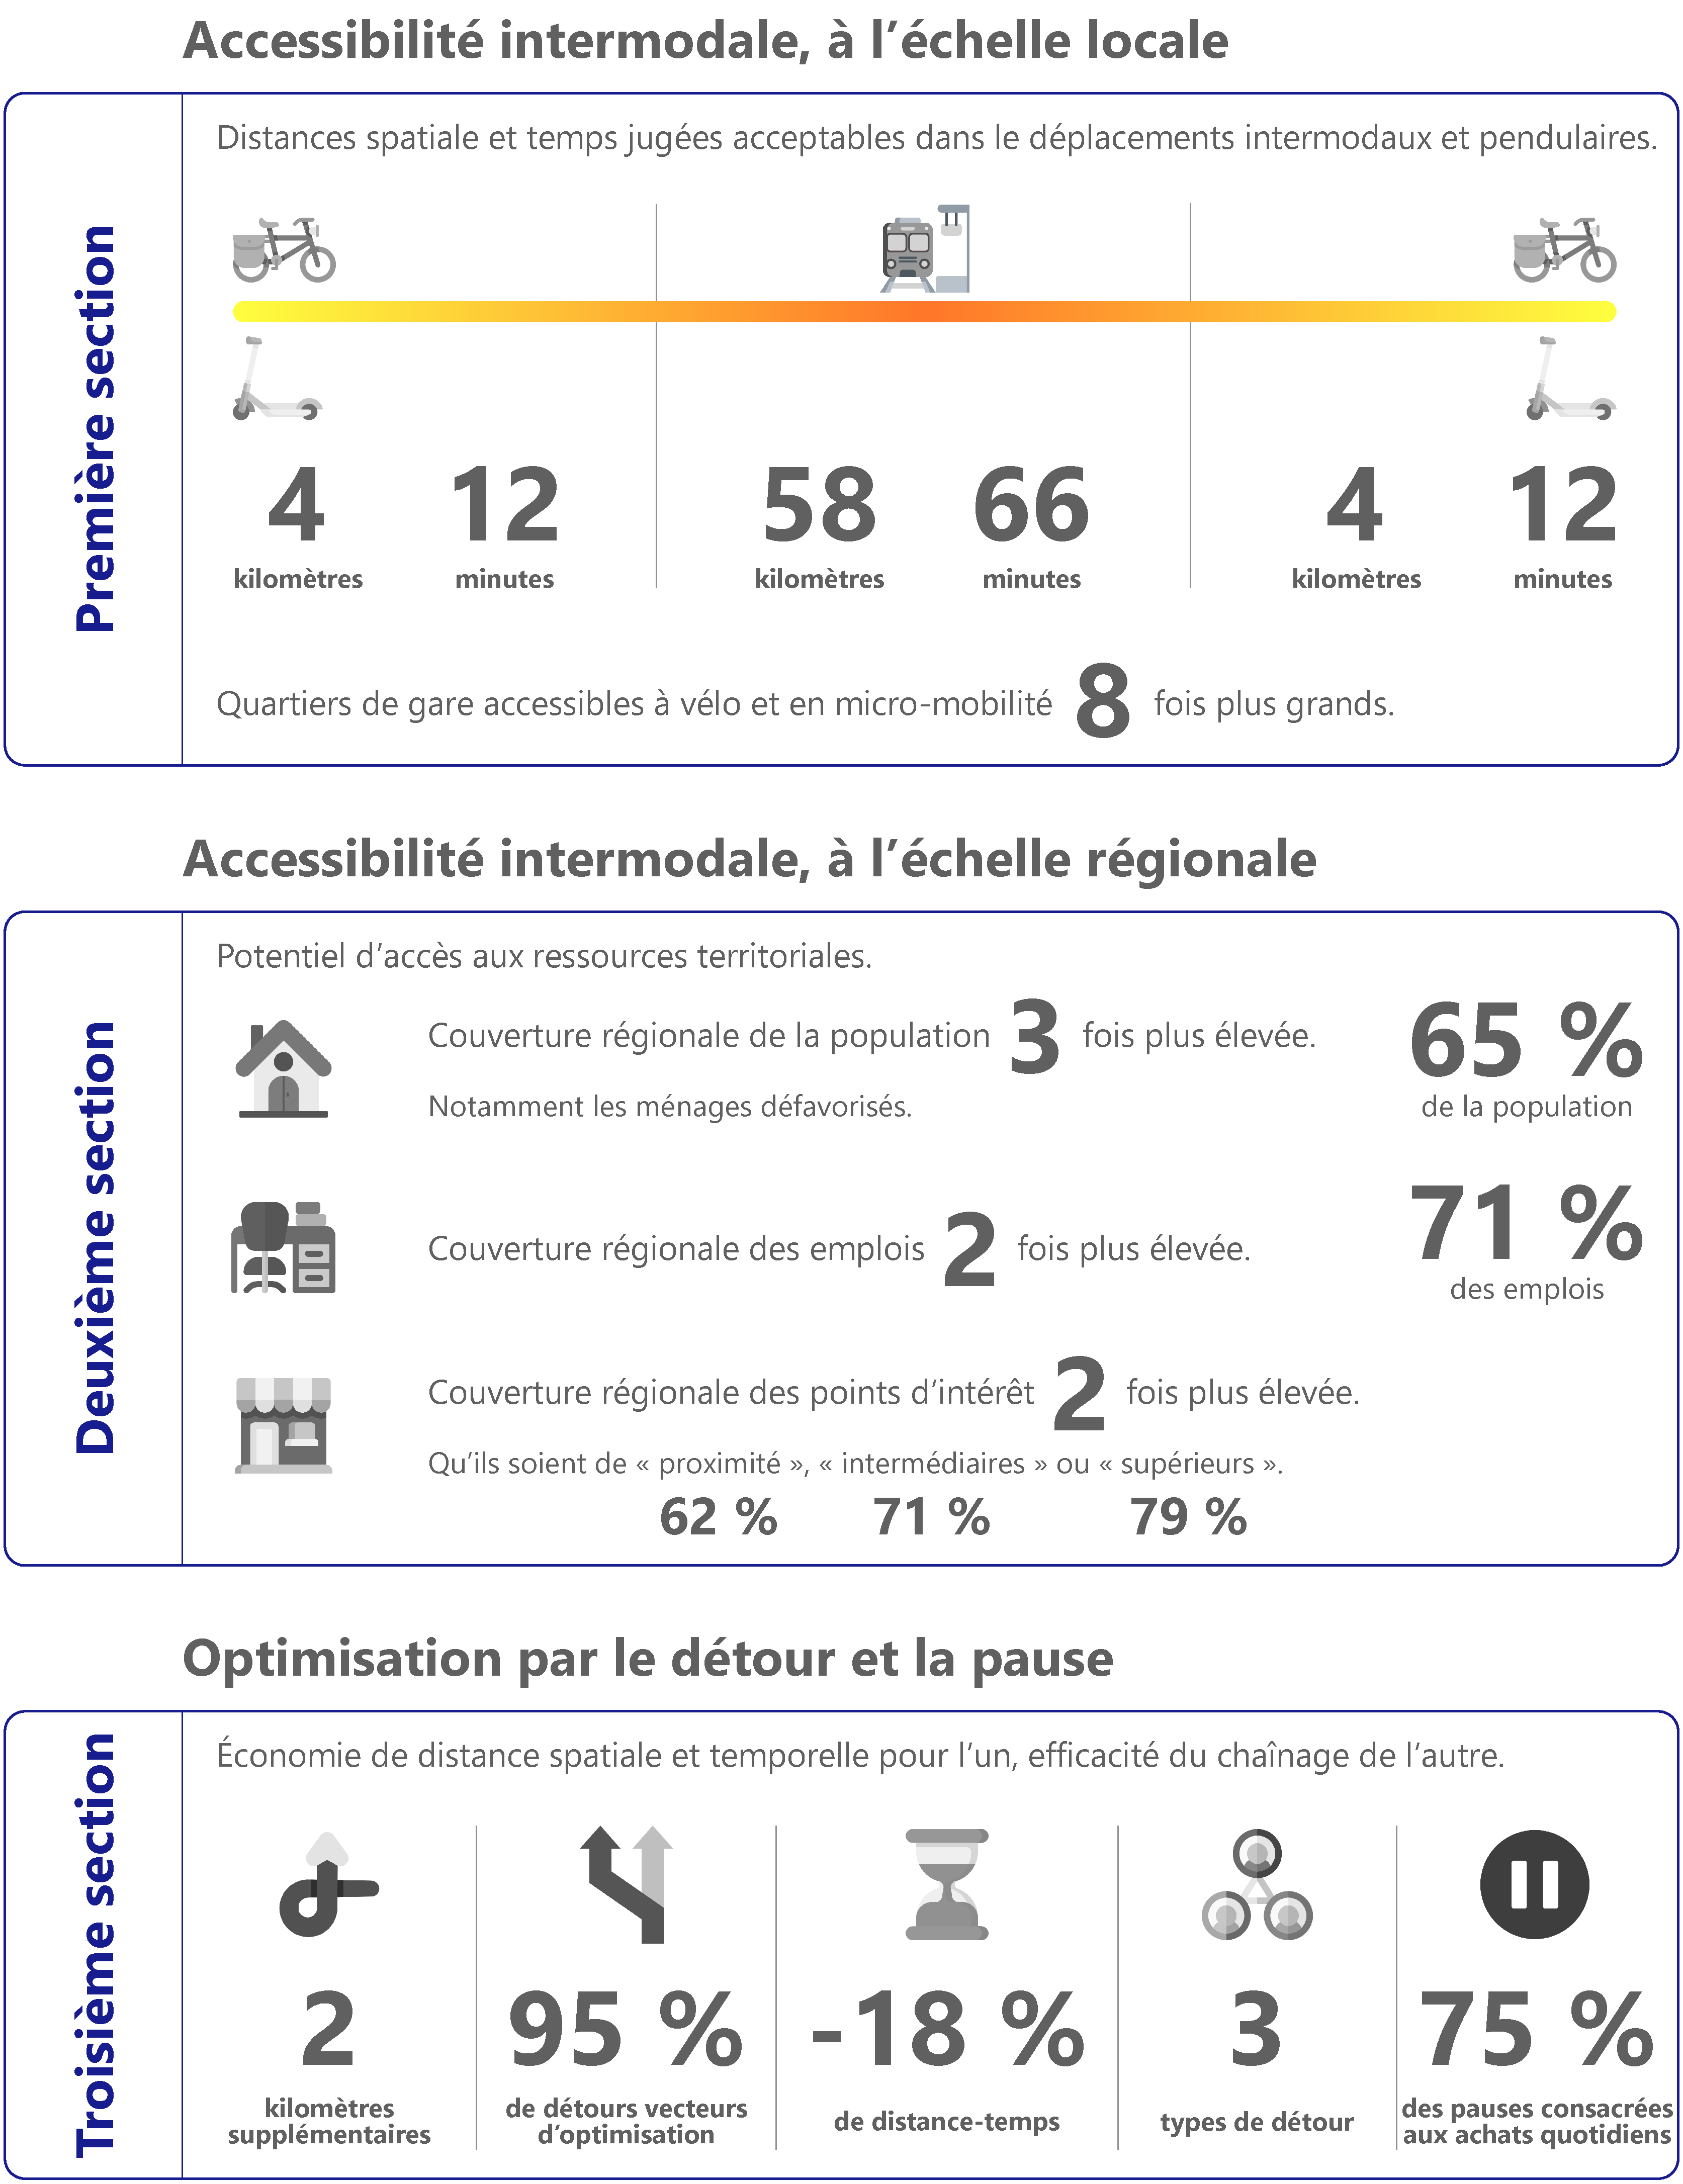
\includegraphics[width=1\columnwidth]{src/Figures/Graphical-abstract/FR_Graphical_abstract_chap5.pdf}}
        \vspace{5pt}
    \end{figure}

    % ___________________________________________
    % Préambule
    \newpage
    \begin{tcolorbox}[colback=white!5!white,
                      colframe=blue!75!blue,
                      title=
                      \bigskip
                      \center{\textbf{Préambule du chapitre~5}}
                      \\
                      \raggedright{\small{Chapitre composé de \pagedifference{chap5:titre}{part2:conclusion} pages, dont \pagedifference{chap5:bibliographie}{part2:conclusion} pages de bibliographie}}
                      \bigskip]
\Large{\textcolor{blue}{\textbf{Résumé~:}}}
    \\
    \small{
Ce chapitre se consacre à l'exploration des périmètres géographiques des quartiers de gare, en interrogeant l'impact de la mobilité individuelle légère, en tant que mode de transfert, sur l'accessibilité locale et intermodale (voir la \hyperref[chap5:aire-cyclable-micromobilite]{section~1}, page~\pageref{chap5:aire-cyclable-micromobilite}). Les données recueillies à partir de l'enquête par questionnaire indiquent que la distance médiane parcourue à vélo et en micro-mobilité est de 2 kilomètres, sur un total de 38 kilomètres. Les parcours effectués en rabattement tendent à être plus longs. L'application d'un modèle de régression a permis de déterminer l'influence de facteurs individuels et contextuels, selon notamment la fréquence d'utilisation, le motif du déplacement et la nomenclature des groupes socioprofessionnels ainsi que sur la variabilité des distances. À l'inverse, la densité démographique ne semble pas détenir d'impact visible sur ces distances.%%Rédigé%%
    \\
Les distances spatiales et temporelles franchies à l'aide de ces modes de déplacement sont ainsi quatre fois supérieures à celles parcourues à pied, redéfinissant de ce fait les limites spatiales autour des nœuds de transport en commun et multipliant par huit la taille des quartiers de gare. Cette extension spatiale permet de desservir, à l'échelle des isochrones, 7,55~\% de la région Hauts-de-France, avec un potentiel maximal de couverture (zones tampons) de 18,48~\%. Les quartiers de gare élargis, combinant les \Guillemets{aires primaires}~et les \Guillemets{aires secondaires}, permettent de desservir plus de la moitié de la population et accordent principalement des gains d'accessibilité aux populations défavorisées. L'analyse souligne par ailleurs que la mobilité individuelle légère, en réponse au défi des \Guillemets{premiers et derniers kilomètres}~des systèmes de transport en commun, double le potentiel d'accès régional aux emplois et aux pôles d'attraction des territoires. Ces gains d'accessibilité illustrent le potentiel de report modal en faveur du réseau ferroviaire, particulièrement dans les territoires dépendants de l'usage et de la place accordée à l'automobile (voir la \hyperref[chap5:accessibilite-intermodale-extension-aire-influence]{section~2}, page~\pageref{chap5:accessibilite-intermodale-extension-aire-influence}).%%Rédigé%%
    \\
L'évaluation des distances a également exploré le rôle joué par la distance, et plus précisément des choix d'itinéraire, dans l'optimisation spatio-temporelle des déplacements, en intégrant des détours et des pauses à vélo ou en micro-mobilité (voir la \hyperref[chap5:detours-pauses-optimisation]{section~3}, page~\pageref{chap5:detours-pauses-optimisation}). Cette approche a permis de dégager trois stratégies d'optimisation par le biais des détours ainsi qu'une typologie de pauses basée sur les motifs déclarés. Les interactions entre le détour, la pause et l'optimisation a permis de mettre en évidence des économies de distance-temps.%%Rédigé%%
    \\
Cette étude nous éclaire alors sur les avantages comparatifs et les enjeux de l'intégration de la mobilité individuelle légère au réseau ferroviaire (voir la \hyperref[chap5:conclusion]{conclusion du chapitre}, page~\pageref{chap5:conclusion}), en documentant non seulement les gains de portée et d'accessibilité régionale enregistrés par ces pratiques intermodales, mais aussi la flexibilité de ces modes de transfert, propices à l'optimisation des distances parcourues lors de la chaîne intermodale.%%Rédigé%%
    }
    \tcblower
\Large{\textcolor{blue}{\textbf{Mots-clés~:}}}
    \\
    \small{
Accessibilité~;
Détour~;
Distance~;
Optimisation~;
Pause~;
Performance du système de transport en commun~;
Potentiel d'accès~;
Premiers et derniers kilomètres~;
Temporalité
    }
    \end{tcolorbox}

    % ___________________________________________
    % 5.*.
    \newpage
    \needspace{1\baselineskip} % Réserve de l'espace
    \addcontentsline{toc}{section}{Introduction du chapitre~5}
    \sectionheader{Introduction du chapitre}
\section*{Introduction du chapitre~5
    \label{chap5:introduction}
    }
    \markright{Introduction du chapitre~5}{}

    % Citation
    \begin{displayquote}
\Guillemets{[\dots] \textsl{que font les acteurs sociaux à l'épreuve de l'espace géographique, que \Guillemets{produisent}~-ils par et pour leur expérience spatiale~? Cela nous a fait découvrir la complexité des technologies mises en œuvre par chaque opérateur social pour arranger, en situation d'action, une configuration où il peut se tenir à bonne distance et en bonne(s) place(s). Ce jeu des distances et des places et l'activité inlassable de délimitation, de découpage, d'évaluation des tailles et des métriques qui l'accompagne toujours, composent, au jour le jour, rien de moins que l'espace de vie des individus en société}.}

\textcolor{blue}{Michel} \textcolor{blue}{\textcite[347]{lussault_homme_2007}}\index{Lussault, Michel|pagebf}. \textsl{L’Homme spatial~: La construction sociale de l’espace humain}. SEUIL, Paris, 400~p. ISBN~: \href{https://search.worldcat.org/fr/title/300390192}{978-2-02-093795-5}
    \end{displayquote}

    % Introduction
\lettrine[lines=3, findent=8pt, nindent=0pt]{\lettrinefont C}{e} chapitre repose sur les implications spatiales de l'intégration de la mobilité individuelle légère au sein des réseaux de \gls{transport en commun}, analysées tant à l'échelle locale que régionale. Ces modes de transfert, envisagés comme une réponse efficace au défi posé par les \Guillemets{premiers et derniers kilomètres} des systèmes de transport public, sont questionnés au regard de leur capacité à étendre les périmètres géographiques du \acrfull{TOD}. Afin d'aborder cette hypothèse générale, nous adoptons tout au long de ce chapitre un regard privilégié sur la notion d'\gls{accessibilité}, en nous concentrant plus particulièrement sur les gains d'accessibilité locale et intermodale associés à ces pratiques intermodales. Dans cette optique, nous nous référons au changement de paradigme défendu par \textcolor{blue}{David} \textcolor{blue}{\textcite[75]{banister_sustainable_2008}}\index{Banister, David|pagebf}~–~à travers un article intitulé \textsl{The Sustainable Mobility Paradigm} et paru dans la revue scientifique \textsl{Transport Policy}~–~qui postule que le modèle du \acrshort{TOD} symbolise une transition d'une conception traditionnelle de la mobilité (\textsl{planning for mobility}) à une approche de la planification urbaine centrée sur l'accessibilité (\textsl{planning for accessibility}). À partir de cette investigation, nous envisageons d'explorer divers aspects permettant de mieux appréhender les gains d'accessibilité attendus, à travers la formulation d'objectifs de recherche dédiés à ce chapitre portant sur les distances et les itinéraires \Guillemets{produits} par \Guillemets{les acteurs sociaux} \textcolor{blue}{\autocite[347]{lussault_homme_2007}}\index{Lussault, Michel|pagebf} ainsi que sur l'accessibilité régionale.%%Rédigé%%

    % Objectifs de recherche
Plusieurs objectifs de recherche viennent structurer ce chapitre de thèse~:
\begin{customitemize}
    \item \textsl{Mesurer l'extension des quartiers de gare, à l'échelle locale}. L'étude portant sur les itinéraires empruntés par les voyageur·se·s intermodaux·les vise à mesurer les gains d'accessibilité aux abords des nœuds de transport en commun, en différenciant les différents véhicules composant la mobilité individuelle légère, afin d'identifier les facteurs influençant les distances parcourues et de déterminer l'étendue des quartiers de gare piétons et cyclables~;
    \item \textsl{Évaluer les gains d'accessibilité, à l'échelle régionale}. L'objectif consiste à comparer la couverture régionale des quartiers de gare en considérant la portée de la marche combinée et de la mobilité individuelle légère. Cette analyse porte notamment sur la quantification du potentiel d'accès de la population aux infrastructures de transport en commun, aux types d'habitat, aux emplois et aux équipements disponibles dans la région~;
    \item \textsl{Examiner les choix d'itinéraire des usager·ère·s} associant l'usage de la mobilité individuelle légère et le réseau de transport en commun, en se focalisant sur la réalisation de détours et de pauses.
\end{customitemize}%%Rédigé%%

    % Annonce du plan 1
Nous procéderons tout d'abord à une analyse statistique des distances spatiales et temporelles caractérisant les déplacements intermodaux recueillis via le questionnaire en ligne conduit, tout en veillant à distinguer les différents segments constitutifs de chaque \gls{déplacement} (\hyperref[chap5:aire-secondaire-quartier-gare]{section~1}, page~\pageref{chap5:aire-secondaire-quartier-gare}). Cette section abordera la délimitation de l'\Guillemets{aire secondaire} des quartiers \acrshort{TOD} à partir des distances individuelles mesurées (\hyperref[chap5:aire-cyclable-micromobilite]{sous-section~1.1}, page~\pageref{chap5:aire-cyclable-micromobilite}) et examinera les caractéristiques individuelles et contextuelles exerçant une influence sur les distances mesurées, au travers d'une modélisation statistique (\hyperref[chap5:regression-distances]{sous-section~1.2}, page~\pageref{chap5:regression-distances}).%%Rédigé%%

    % Annonce du plan 2
Suivant la détermination de la taille des quartiers de gare selon des critères de distances spatiales et temporelles acceptables, nous évaluerons l'impact de ces gains d'accessibilité à l'échelle de la région Hauts-de-France (\hyperref[chap5:accessibilite-intermodale-extension-aire-influence]{section~2}, page~\pageref{chap5:accessibilite-intermodale-extension-aire-influence}). Nous nous intéresserons au potentiel de report modal en faveur du système ferroviaire, en examinant la desserte de la population et l'inclusivité sociale de cette accessibilité intermodale (\hyperref[chap5:couverture-population]{sous-section~2.1}, page~\pageref{chap5:couverture-population}) ainsi que les opportunités d'accès aux points d'attraction de la région (\hyperref[chap5:couverture-population]{sous-section~2.2}, page~\pageref{chap5:accessibilite-emplois}).%%Rédigé%%

    % Annonce du plan 3
La dernière phase de ce chapitre sera consacrée à l'étude des choix d'itinéraire en dirigeant notre attention sur un sous-échantillon de parcours à vélo ou en micro-mobilité autour des stations de transport en commun. L'intérêt de la \hyperref[chap5:detours-pauses-optimisation]{section~3} (page~\pageref{chap5:detours-pauses-optimisation}) est d'éclairer les motivations de tels détours et d'arrêts intermédiaires. Pour cela, nous nous intéresserons au lien existant dans la littérature scientifique entre le détour, la pause et l'optimisation du mouvement (\hyperref[chap5:enjeux-detours-pauses]{sous-section~3.1}, page~\pageref{chap5:enjeux-detours-pauses}). Nous présenterons ensuite notre méthode d'analyse statistique (\hyperref[chap5:methodes-statistiques]{sous-section~3.2}, page~\pageref{chap5:methodes-statistiques}) destinée à vérifier si ces détours et ces pauses contribuent à des gains de distance-temps (\hyperref[chap5:strategies-optimisation]{sous-section~3.3}, page~\pageref{chap5:strategies-optimisation}), avant de discuter de ces observations (\hyperref[chap5:discussion-detours-pauses-optimisation]{sous-section~3.4}, page~\pageref{chap5:discussion-detours-pauses-optimisation}).%%Rédigé%%

    % Annonce du plan 4
En conclusion, nous synthétiserons les principaux enseignements de ce chapitre qui nous éclairent sur l'extension des quartiers de gare et leurs implications spatiales au sein du périmètre régional (\hyperref[chap5:conclusion]{conclusion du chapitre~5}, page~\pageref{chap5:conclusion}).%%Rédigé%%

     % ___________________________________________
    % 5.1.
    \newpage
    \needspace{1\baselineskip} % Réserve de l'espace
    \sectionheader{Détermination d'une aire secondaire}
\section{Mesure de l'\Guillemets{aire secondaire} autour du quartier de gare et potentiel d’usage intermodal par les voyageur·se·s
    \label{chap5:aire-secondaire-quartier-gare}
    }

    % Introduction
Dans cette première section, nous nous attachons à explorer la manière dont les distances spatio-temporelles jugées acceptables à \gls{vélo} et en \gls{micro-mobilité}, en tant que modes de transfert vers et depuis les réseaux de transport en commun, peuvent définir l'extension des quartiers de gare. En analysant les déplacements domicile-travail et domicile-études, nous sommes en mesure de déterminer la portée effective de ces modes de déplacement et ainsi de déduire leur capacité à élargir l'aire d'influence, dénommée \Guillemets{aire secondaire}, des gares de la région Hauts-de-France. En nous appuyant sur les réponses recueillies dans le cadre du questionnaire mené auprès des usager·ère·s intermodaux·ales, cette étude veille à quantifier, dans un premier temps, la distribution des distances parcourues, comme détaillé dans la \hyperref[chap5:aire-cyclable-micromobilite]{première sous-section délimitant l'extension des quartiers de gare} (page~\pageref{chap5:aire-cyclable-micromobilite}). Dans un second temps, elle révèle, à travers la \hyperref[chap5:regression-distances]{seconde sous-section modélisant les facteurs influençant la distance} (page~\pageref{chap5:regression-distances}), la variation des distances en fonction de divers facteurs liés aux comportements de mobilité, à l'environnement urbain et aux caractéristiques socio-démographiques.%%Rédigé%%

    % 5.1.1.
    \needspace{1\baselineskip} % Réserve de l'espace
\subsection{Mesure de l'aire cyclable acceptable aux abords des nœuds de transport en commun
    \label{chap5:aire-cyclable-micromobilite}
    }

    % Introduction
Notre objectif premier consiste à mesurer la zone de pertinence de la mobilité individuelle légère aux abords des nœuds de transport en commun. En fondant l'analyse des distances sur les réponses de ces utilisateur·rice·s ayant participé à notre enquête, nous avons représenté et étudié la distribution des distances spatiales parcourues pour chaque segment composant leurs déplacements pendulaires. Les statistiques descriptives qui s'ensuivent sont ainsi basées sur 217 réponses et 262 trajets à vélo ou en micro-mobilité qui nous ont permis de déterminer la portée effective de ces modes de déplacement et, par conséquent, de définir les contours d'un quartier \acrshort{TOD} étendu.%%Rédigé%%

    % 5.1.1.1.
    \needspace{1\baselineskip} % Réserve de l'espace
\subsubsection*{Distances spatiales parcourues à l'aide de la mobilité individuelle légère
    \label{chap5:distances-spatiales-parcourues}
    }

    % Figure violons distances
    \begin{figure}[h!]\vspace*{4pt}
        \caption{Diagrammes en violon des distances de rabattement et de diffusion parcourues par les navetteur·se·s intermodaux·les en mobilité individuelle légère.}
        \label{fig-chap5:diagrammes-violons}
        \centerline{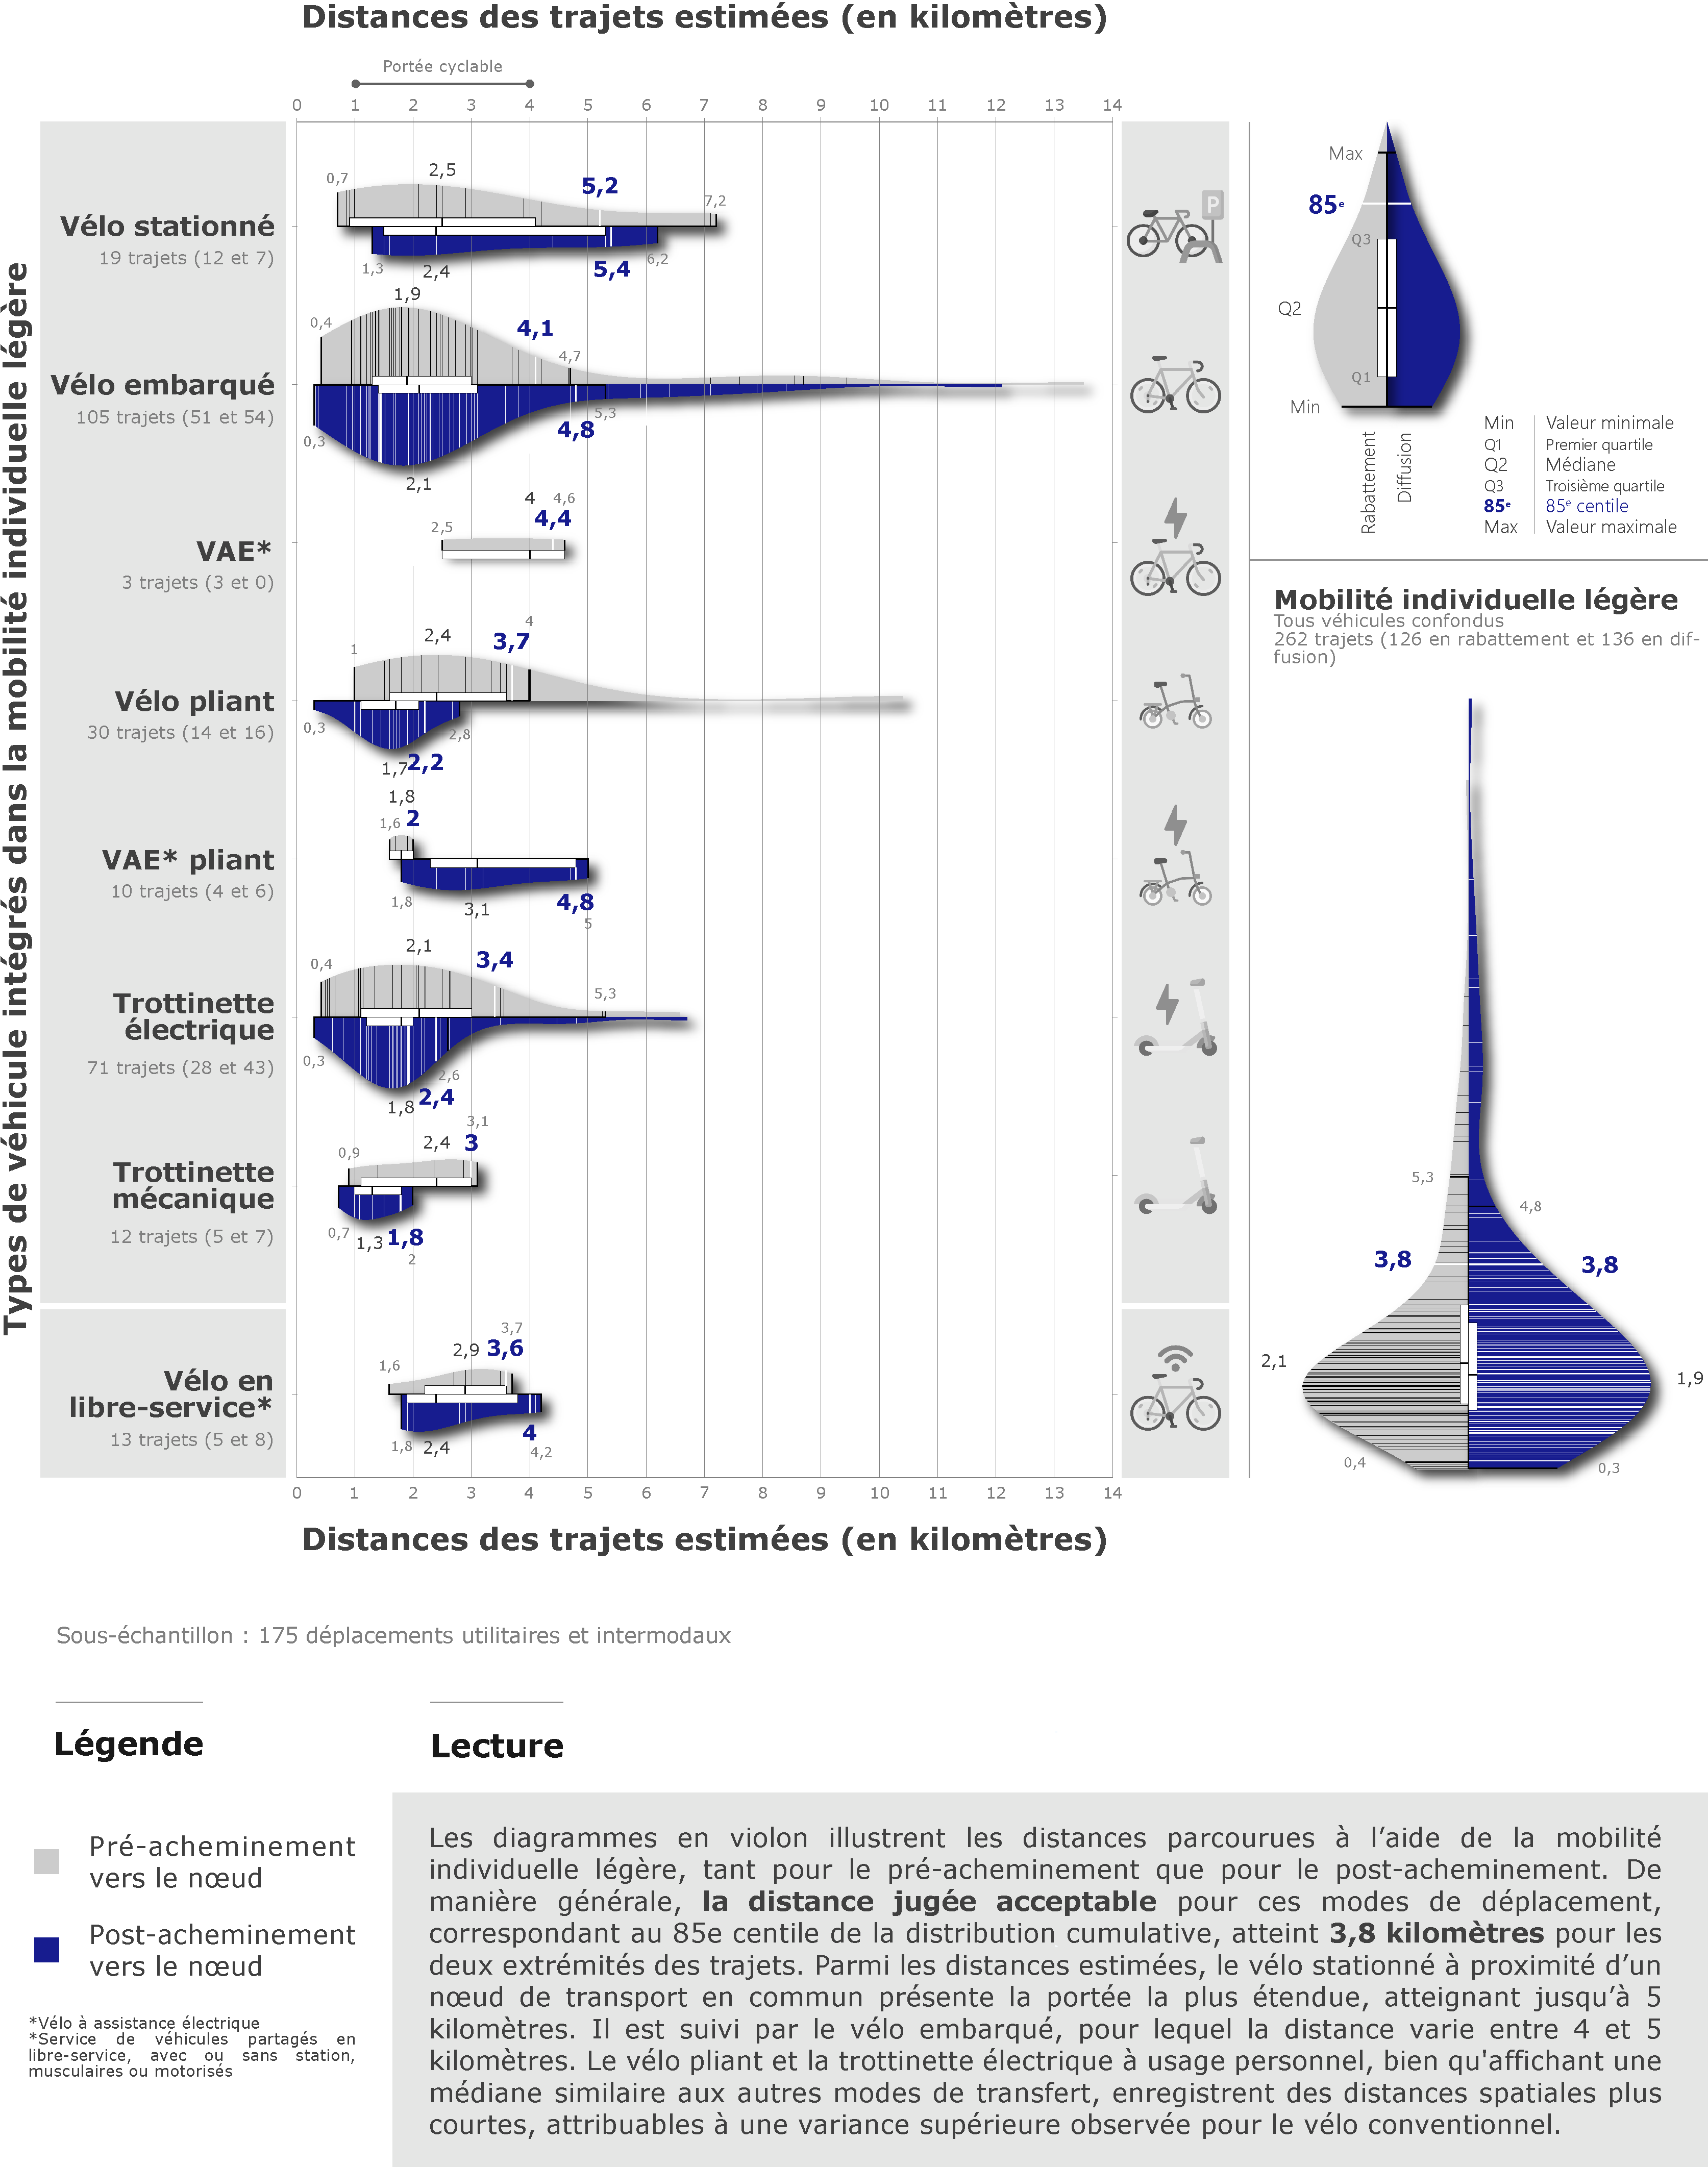
\includegraphics[width=1\columnwidth]{src/Figures/Chap-5/FR_Distances_Violons_Navetteurs.png}}
        \vspace{5pt}
        \begin{flushright}\scriptsize{
        Auteur~: \textcolor{blue}{Dylan Moinse (2023)}
        }\end{flushright}
    \end{figure}
    
    % Statistiques distances parcourues
L'examen des distances participant aux navettes domicile-travail effectuées en mobilité individuelle légère, tant pour le pré-acheminement que pour le post-acheminement, révèle l'appropriation d'un périmètre géographique de pertinence autour des nœuds de transport public, qui s'étend sur trois à quatre kilomètres de part et d'autre. De manière plus précise, la distance médiane réalisée à vélo ou en micro-mobilité est de 2 kilomètres, se décomposant en 2,1 kilomètres pour le trajet en \gls{rabattement} et 1,9 kilomètre pour le segment en \gls{diffusion}. Toutefois, il convient de considérer que la distance jugée acceptable, qui définit la portée de ces modes de déplacement, est davantage déduite du 85\textsuperscript{e} centile de la distribution cumulative des distances parcourues, comme introduit dans la \hyperref[chap3:quartiers-gare-distances]{section consacrée à la spatialisation des quartiers de gare} (page~\pageref{chap3:quartiers-gare-distances}) du \hyperref[chap3:titre]{chapitre~3} (page~\pageref{chap3:titre}). À partir de cette mesure, la distance critique pour la mobilité individuelle légère, tant pour les premiers que pour les derniers kilomètres, est estimée à 3,8 kilomètres pour chaque \gls{itinéraire} (voir l'\hyperref[fig-chap5:diagrammes-violons]{illustration~\ref{fig-chap5:diagrammes-violons}}, page~\pageref{fig-chap5:diagrammes-violons}). En conséquence, le rayon d'action autour des quartiers de gare, adapté à l'usage du vélo et de la micro-mobilité, atteint 3,8 kilomètres, contre seulement 1,3 kilomètre lorsqu'il est mesuré pour la marche. Il est à noter également que des variations mineures sont observées entre les distances parcourues dans les deux scénarios étudiés~: le trajet en rabattement depuis le domicile affiche généralement des distances plus longues, variant de 0,4 à 5,3 kilomètres, tandis que les distances pour les trajets en direction du lieu d'activité s'étendent de 0,3 à 4,8 kilomètres.%%Rédigé%%

    % Distances selon le type de MIL
En considérant l'ensemble des déplacements ayant un motif utilitaire ou étant destiné aux loisirs, notre analyse s'est appuyée sur la représentation de la fonction d'impédance\footnote{
    La fonction d'impédance peut être utilisée dans la modélisation des transports pour exprimer comment la friction de la distance spatiale ou temporelle influence la probabilité ou la quantité de déplacements. Elle part du postulat selon lequel les individus ne cessent pas instantanément de se déplacer après une certaine distance spatio-tmeporelle, mais que leur probabilité de déplacement diminue graduellement. Il s'agit d'une fonction décroissante qui quantifie la diminution du nombre de déplacements avec l'augmentation du coût de déplacement. Dans leur article scientifique nommé \foreignlanguage{english}{\textsl{The Influence of the Impedance Function on Gravity-based Pedestrian Accessibility Measures: A Comparative Analysis}}, \textcolor{blue}{\textcite[758]{vale_influence_2017}}\index{Vale, David~S.|pagebf}\index{Pereira, Mauro|pagebf} ont analysé vingt mesures d'accessibilité gravitaire, en variant les fonctions d'impédance et leurs paramètres associés. L'analyse factorielle produite a montré que les mesures produisent des résultats similaires pour identifier la \Guillemets{distance acceptable à pied}. En suivant leurs préconisations s'agissant des études spatiales sur l'accessibilité urbaine, nous avons appliqué la fonction d'impédance gaussienne cumulative pour modéliser la perception des distances dans les déplacements intermodaux.
}, associée à la quantification des coûts liés à un déplacement. Ce modèle permet principalement de prédire le choix modal et les choix d'itinéraire basés sur les résistances rencontrées sur chaque option de trajet. Ainsi, l'analyse statistique a permis de déterminer que la réalisation d'un trajet en mobilité individuelle légère et connecté au réseau de transport en commun est relativement peu coûteuse pour l'usager·ère lorsque le rayon de distance spatiale est compris entre 0,8 et 4,2 kilomètres concernant la phase de pré-acheminement, et entre 0,5 et 3,3 kilomètres en post-acheminement (voir l'\hyperref[fig-chap5:impedance-distances]{illustration~\ref{fig-chap5:impedance-distances}}, page~\pageref{fig-chap5:impedance-distances}). L'examen graphique des données cumulatives révèle que le vélo conventionnel détient une portée acceptable allant de 0,8 à 4,8 kilomètres en rabattement et de 1,3 à 5,2 kilomètres en diffusion. Par contraste, la visualisation de la fonction d'impédance pour le vélo pliant suggère que sa portée est moins coûteuse, d'une part entre 1,1 et 4 kilomètres et d'autre part, entre 0,4 et 2,8 kilomètres. S'agissant de la \acrfull{TEP}, les intervalles de distance spatiale associés sont respectivement compris entre 0,5 et 3 kilomètres et entre 0,3 et 2,7 kilomètres. La marche quant à elle renvoie à une portée maximisée entre 0,1 et 1,2 kilomètre et entre 0,2 et 1,1 kilomètre. Il apparaît ainsi que la pratique de la mobilité individuelle légère et de la marche combinée est structurée de manière hiérarchique selon la distance parcourue. En effet, le vélo conventionnel se distingue comme le mode cyclable privilégié pour les trajets les plus longs et qui impliquent une certaine distance minimale, suivi par le vélo pliant, la \acrshort{TEP}, le \acrfull{VLS} et le \acrfull{VFF}. La marche occupe la dernière position dans cette stratification, étant majoritairement adoptée pour les distances les plus courtes. Notons cependant que les trajets pédestres en phase de post-acheminement, tels que déclarés dans le cadre de cette enquête, sont généralement précédés de l'utilisation d'un vélo classique avant l'accès à la station de transport en commun.%%Rédigé%%

    % Figure fonctions d'impédance distances - fonction de décroissance
    \begin{figure}[h!]\vspace*{4pt}
        \caption{Détermination de l'impédance des distances de rabattement et de diffusion parcourues par les voyageur·se·s intermodaux·les en mobilité individuelle légère.}
        \label{fig-chap5:impedance-distances}
        \centerline{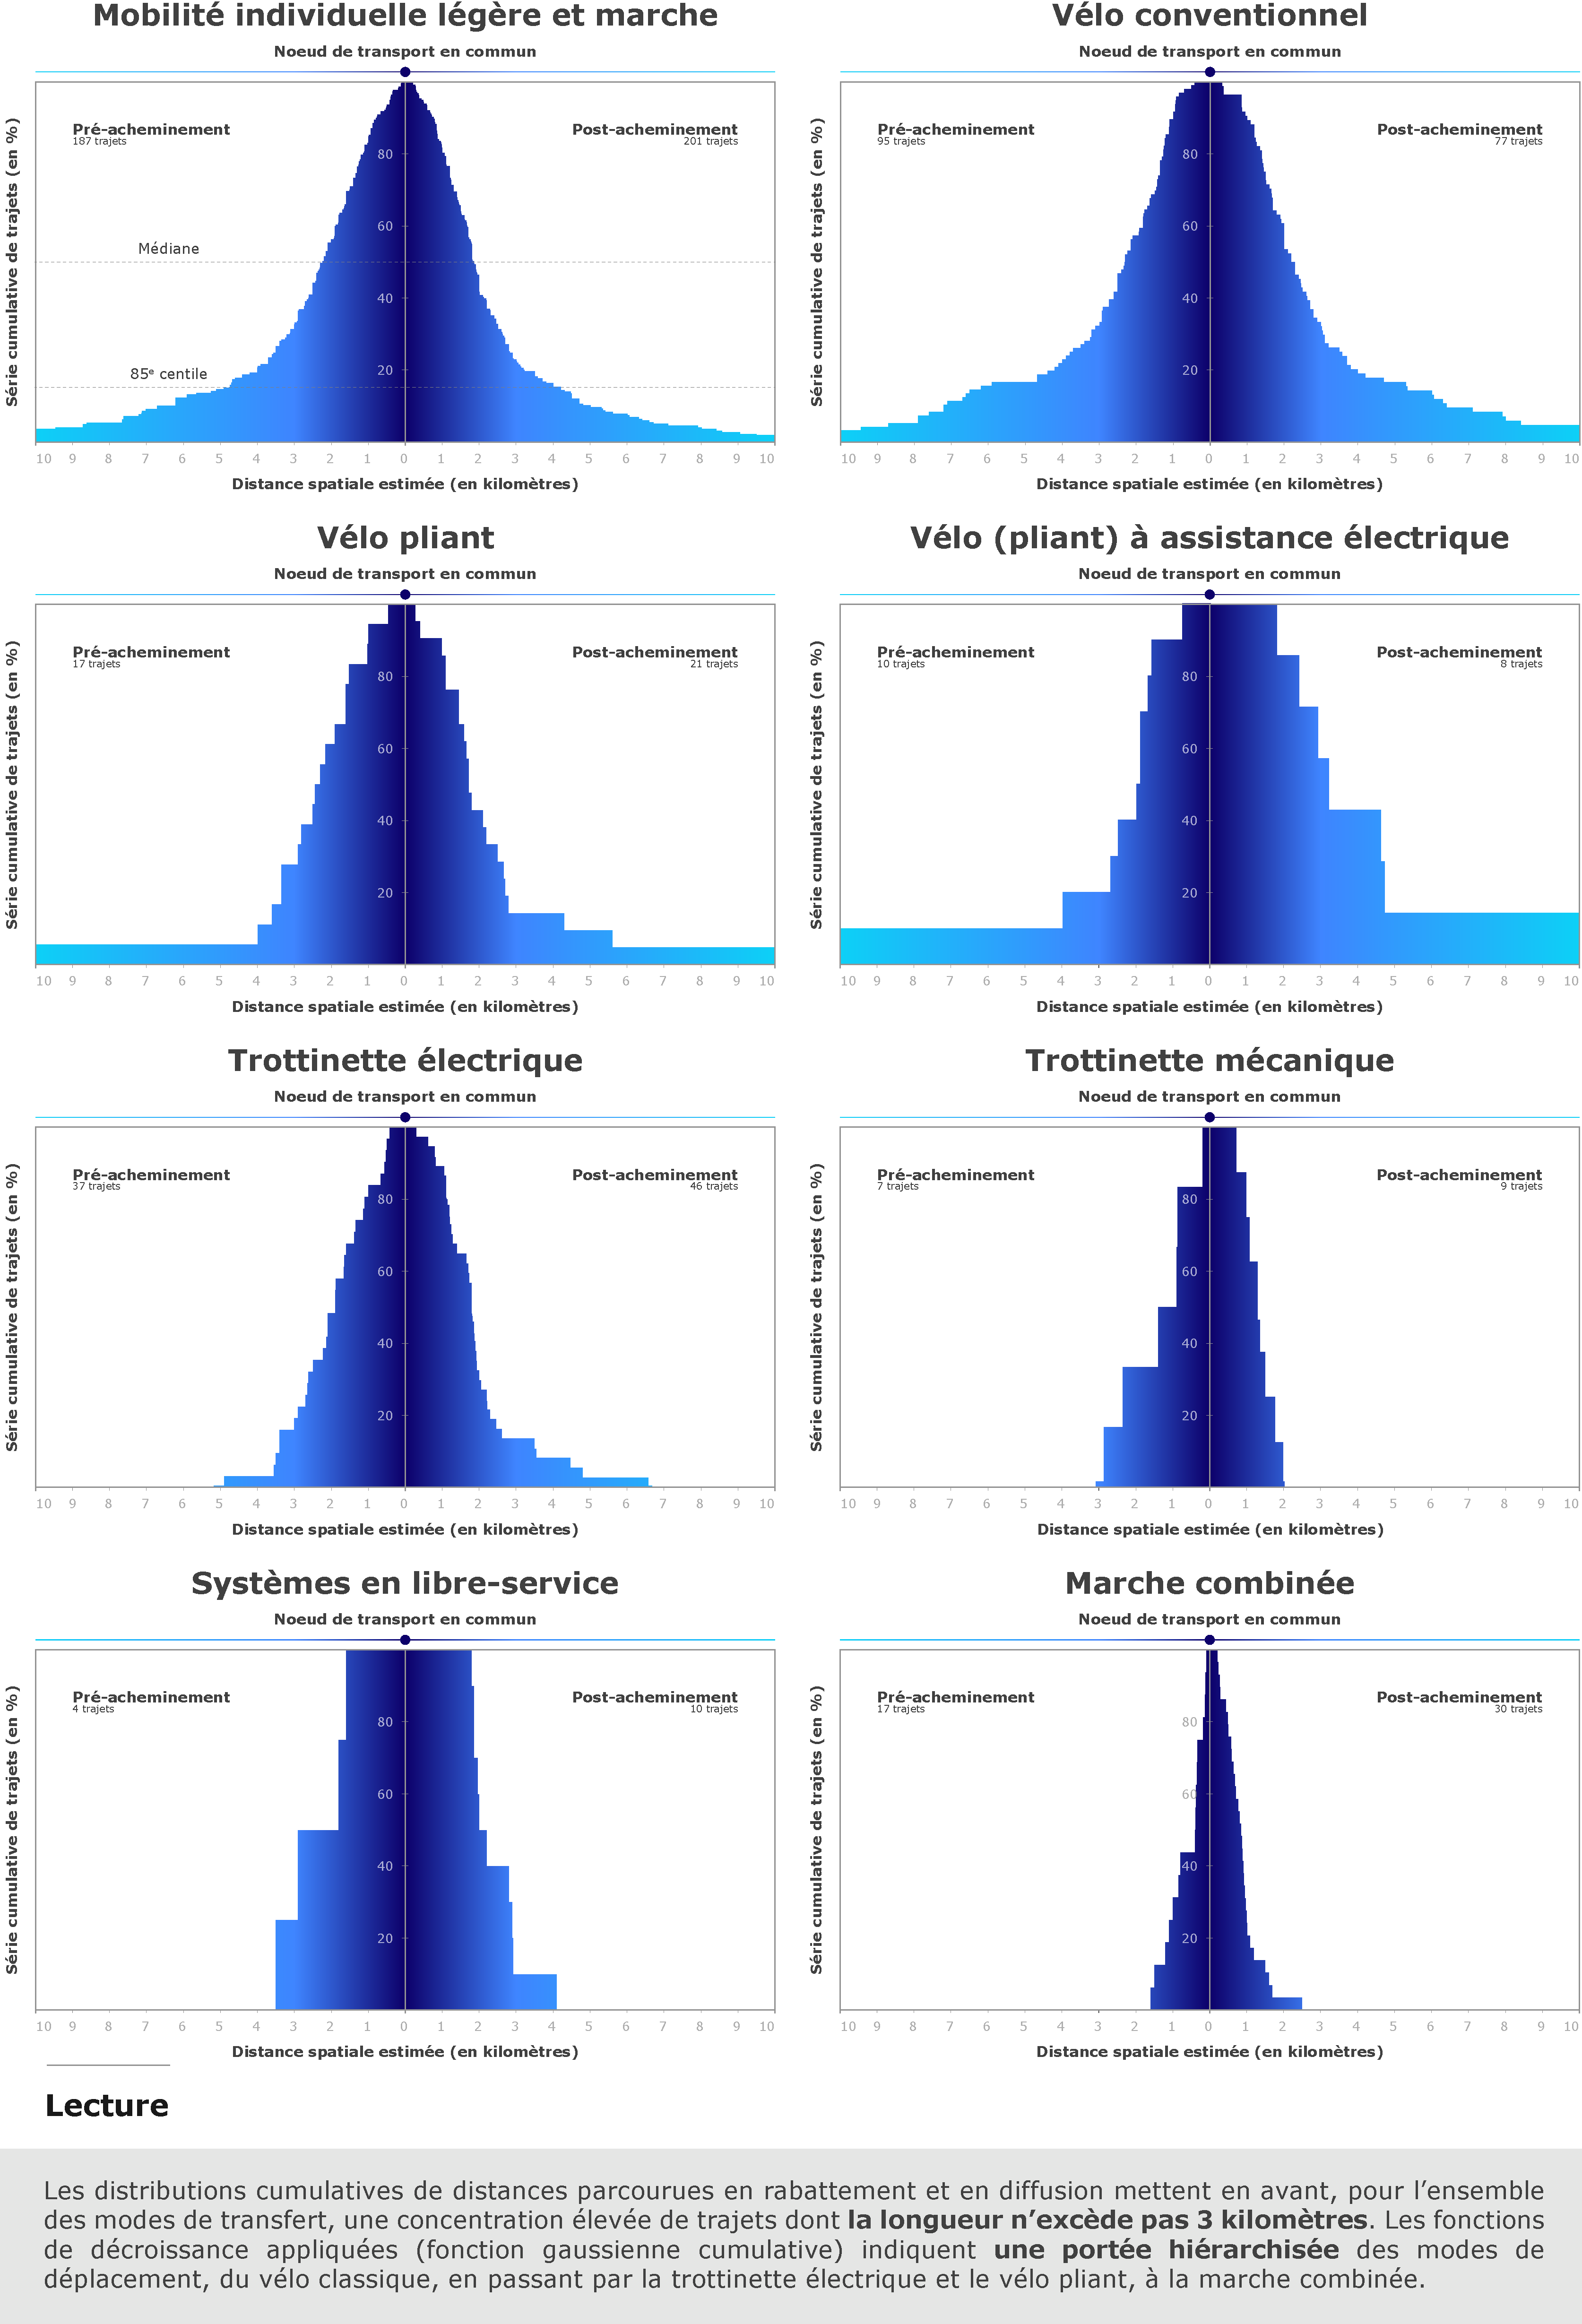
\includegraphics[width=1\columnwidth]{src/Figures/Chap-5/FR_Distances_Impedance.pdf}}
        \vspace{5pt}
        \begin{flushright}\scriptsize{
        Auteur~: \textcolor{blue}{Dylan Moinse (2024)}
        }\end{flushright}
    \end{figure}

    % Symétrie de gains de distance selon l'embarquement
Un aspect supplémentaire considéré dans cette étude sur les distances concerne l'effet d'asymétrie ou de symétrie des bénéfices en termes d'accessibilité offerts par la mobilité individuelle légère. La faculté de transporter son véhicule sur le réseau de transport en commun, ou de disposer d'un second vélo durant la phase de diffusion, permet de bénéficier de distances accrues tant dans les premiers que dans les derniers kilomètres d'un déplacement intermodal. L'analyse des configurations modales adoptées au cours des deux segments démontre que, de manière générale, 66,97~\% des voyageur·se·s ont recours au même mode de déplacement lors des deux étapes concernées. Ce phénomène est particulièrement prévalent parmi les usager·ère·s du vélo pliant (82,61~\%) et de la \acrshort{TEP} (79,49~\%). Le vélo classique figure en troisième position, avec 71,96~\% des cyclistes les utilisant à la fois en rabattement et en diffusion.%%Rédigé%%

    % Suite symétrie de gains de distance
Ce schéma illustre un certain avantage comparatif des véhicules les plus légers et les plus aisément embarquables à bord des modes collectifs~: le vélo pliant et la \acrshort{TEP} constituent une solution adaptée à la problématique spécifique des \Guillemets{derniers kilomètres}, doublant ainsi la portée de leur efficacité de chaque côté de la station. Nous avons également identifié de telles pratiques de mobilité dans la région Provence-Alpes-Côte d'Azur, où 85~\% des voyageur·se·s ferroviaires se déplaçant en \acrshort{TEP} ou en trottinette mécanique utilisent ces \acrshort{EDP} pour leurs premiers et pour leurs derniers kilomètres, contre seulement 34~\% des passager·ère·s dans l'ensemble \textcolor{blue}{\autocite[185]{moinse_intermodal_2022}}\index{Moinse, Dylan|pagebf}\index{Goudeau, Matthieu|pagebf}\index{L'Hostis, Alain|pagebf}\index{Leysens, Thomas|pagebf}.%%Rédigé%%

    % Symétrie questionnaire parcours commentés
En approfondissant l'analyse de la question \Guillemets{\textsl{Pour quelles raisons avez-vous embarqué votre véhicule~?}} intégrée au questionnaire, 87,22~\% (157 participant·e·s) des usager·ère·s ayant choisi d'emporter leur vélo ou leur micro-véhicule ont indiqué que la motivation principale était la possibilité de l'utiliser à la sortie de la station, en raison de distances jugées longues. Par ailleurs, 6,11~\% des répondant·e·s (11 participant·e·s) ont motivé leur choix par des infrastructures de stationnement peu sécurisées, tandis que 5~\% d'entre elleux (9 participant·e·s) ont signalé l'absence de stationnement à proximité immédiate de la station. En outre, la raison principale justifiant l'embarquement de la \acrshort{TEP} figure également lors du parcours commenté réalisé avec le participant \(PCTE_{2}\). Ce dernier justifie l'utilisation combinée de cet \acrshort{EDP} avec le métro pour atteindre ses deux destinations à Villeneuve d'Ascq, bien qu'il reconnaisse que son trajet en rabattement aurait pu être effectué à pied.%%Rédigé%%

    % Distances selon le type de TC
Si l'amplitude des distances spatiales parcourues par les voyageur·se·s intermodaux·les employant la mobilité individuelle légère diffère selon le type de véhicule, elle est également influencée par la nature du système de transport en commun, en accord avec la littérature scientifique \textcolor{blue}{\autocite[105]{flamm_public_2014}}\index{Flamm, Bradley~J.|pagebf}\index{Rivasplata, Charles~R.|pagebf}. En effet, il ressort que les gares intégrées au réseau \acrshort{TGV} disposent d'une zone d'influence s'étendant jusqu'à un rayon de quatre kilomètres, tandis que celles desservies uniquement par le réseau \acrshort{TER} ou \acrshort{TERGV} présentent des rayons d'environ trois kilomètres. Concernant les systèmes de transport en commun urbain sur rail, tels que le métro et le tramway, le rayon moyen est estimé à deux kilomètres. En nous référant à la segmentation de la \acrfull{DRG} (voir la \hyperref[chap4:part-modale-gares-centre-periurbain]{section dédiée à la part modale de la mobilité individuelle légère en transfert dans les types de gare}, page~\pageref{chap4:part-modale-gares-centre-periurbain} du \hyperref[chap5:titre]{chapitre~5}, page~\pageref{chap5:titre}), établie par \textcolor{blue}{\textcite{sncf_gares__connexions_gares_2024}}\index{SNCF Gares \& Connexions@\textsl{SNCF Gares \& Connexions}|pagebf}, qui classe les gares françaises en différents groupes selon divers critères, nous pouvons observer que la distance jugée acceptable à vélo ou en micro-mobilité, établie au 85\textsuperscript{e} centile, diminue proportionnellement au niveau de service en gare (voir le \hyperref[table-chap5:distances-type-tc]{tableau~\ref{table-chap5:distances-type-tc}}, page~\pageref{table-chap5:distances-type-tc}). Ainsi, les gares de catégorie~\(a\) présentent une distance acceptable de 4,8 kilomètres, tandis que celles de catégorie~\(b\) et de catégorie~\(c\) affichent respectivement des distances de 4,26 kilomètres et de 3,8 kilomètres.%%Rédigé%%

    % Tableau distances selon TC
% Tableau distances selon TC
%%Rédigé%%
        \begin{table}[h!]
        \centering
        \renewcommand{\arraystretch}{1.5}
        \resizebox{\columnwidth}{!}{
        \begin{tabular}{p{0.38\columnwidth}p{0.1\columnwidth}p{0.12\columnwidth}p{0.1\columnwidth}p{0.1\columnwidth}p{0.1\columnwidth}p{0.1\columnwidth}}
        %\hline
    \rule{0pt}{15pt} \multirow{1.5}{*}{\small{\textbf{\textcolor{blue}{Typologie}}}} & \small{\textbf{\textcolor{blue}{25\textsuperscript{e} centile}}} & \multirow{1.5}{*}{\small{\textbf{\textcolor{blue}{Médiane}}}} & \small{\textbf{\textcolor{blue}{85\textsuperscript{e} centile}}} & \multirow{1.5}{*}{\small{\textbf{\textcolor{blue}{Min.}}}} &  \multirow{1.5}{*}{\small{\textbf{\textcolor{blue}{Max.}}}} &  \multirow{1.5}{*}{\textbf{\textcolor{blue}{$\sigma$}}}\\
        \hline
    \small{Tous types de réseau confondus} & \multirow{1.5}{*}{\small{1,30}} & \multirow{1.5}{*}{\small{2,00}} & \multirow{1.5}{*}{\small{\textbf{3,80}}} & \multirow{1.5}{*}{\small{0,20}} & \multirow{1.5}{*}{\small{54,60}} & \multirow{1.5}{*}{\small{15,12}}\\
        \hdashline
    \small{Gares de catégorie~\(a\)} & \small{1,70} & \small{2,40} & \small{\textbf{4,80}} & \small{0,37} & \small{54,60} & \small{24,38}\\
    \small{Gares de catégorie~\(b\)} & \small{1,42} & \small{1,94} & \small{\textbf{4,26}} & \small{0,21} & \small{39,90} & \small{4,90}\\
    \small{Gares de catégorie~\(c\)} & \small{1,33} & \small{1,66} & \small{\textbf{3,80}} & \small{0,78} & \small{46,10} & \small{10,23}\\
    \small{Arrêts de métro et de tramway} & \multirow{1.5}{*}{\small{0,67}} & \multirow{1.5}{*}{\small{1,05}} & \multirow{1.5}{*}{\small{\textbf{2,37}}} & \multirow{1.5}{*}{\small{0,20}} & \multirow{1.5}{*}{\small{9,10}} & \multirow{1.5}{*}{\small{1,84}}\\
        \hline
        \end{tabular}}
    \caption{Distribution des distances spatiales franchies en rabattement ou en diffusion, dans le cadre de déplacements pendulaires, en fonction de la nature du système de transport en commun et du type de gare.}
    \label{table-chap5:distances-type-tc}
        \vspace{5pt}
        \begin{flushleft}\scriptsize{
        \textcolor{blue}{Note~:} $\sigma$~correspond à l'écart-type.
        \\
        \textcolor{blue}{Lecture~:} les distances spatiales franchies en rabattement ou en diffusion varient significativement selon le type de gare et de réseau~: les gares de classe~\(a\) enregistrent les distances les plus élevées, tandis que les arrêts de transport urbain sur rail affichent des distances nettement inférieures.
        }\end{flushleft}
        \begin{flushright}\scriptsize
        Auteur~: \textcolor{blue}{Dylan Moinse (2023)}
        \end{flushright}
        \end{table}%%Rédigé%%

    % Littérature
Lors de la comparaison des distances estimées dans notre étude avec celles rapportées par la littérature scientifique, il apparaît que nos recherches s'accordent avec les résultats préalablement établis concernant les pratiques intermodales. Effectivement, la zone de pertinence géographique située autour des gares, estimée entre trois et quatre kilomètres, trouve une validation dans les travaux de \textcolor{blue}{\textcite[234]{keijer_how_2000}}\index{Keijer, Majanka|pagebf}\index{Rietveld, Piet|pagebf}, de \textcolor{blue}{\textcite[359]{givoni_access_2007}}\index{Givoni, Moshe|pagebf}\index{Rietveld, Piet|pagebf}, de \textcolor{blue}{\textcite[23]{debrezion_modelling_2009}}\index{Debrezion, Ghebreegziabiher|pagebf}\index{Pels, Eric|pagebf}\index{Rietveld, Piet|pagebf}, de \textcolor{blue}{\textcite[213]{kager_characterisation_2016}}\index{Kager, Roland|pagebf}\index{Bertolini, Luca|pagebf}\index{te Brömmelstroet, Marco|pagebf} et de \textcolor{blue}{\textcite[42]{nielsen_bikeability_2018}}\index{Nielsen, Thomas Alexander Sick|pagebf}\index{Skov-Petersen, Hans|pagebf}. Plus précisément, notre analyse par impédance a révélé des rayons de distances spatiales où la mobilité individuelle légère présente un coût relativement moindre, s'échelonnant de 0,8 à 4,2 kilomètres en rabattement, ce qui correspond aux observations de \textcolor{blue}{Karel} \textcolor{blue}{\textcite[282]{martens_bicycle_2004}}\index{Martens, Karel|pagebf}, qui fait état de rayons allant de 1,1 à 4,2 kilomètres en pré-acheminement, aussi bien en Allemagne, aux Pays-Bas qu'au Royaume-Uni, ou encore de \textcolor{blue}{Christian} \textcolor{blue}{\textcite[14]{gioria_etude_2016}}\index{Gioria, Christian|pagebf} qui déduit une distance maximale de 5 kilomètres en rabattement comme en diffusion, à l'aide du vélo en France. Par ailleurs, \textcolor{blue}{Piet} \textcolor{blue}{\textcite[73]{rietveld_accessibility_2000}}\index{Rietveld, Piet|pagebf} souligne l'existence d'une asymétrie entre les extrémités d'un déplacement intermodal, le segment depuis le domicile étant plus propice à l'utilisation du vélo avec des distances variant de 1,2 à 3,7 kilomètres. Cette asymétrie se retrouve également dans nos résultats statistiques. En ce qui concerne la notion d'acceptabilité sociale des distances maximales, qui repose sur un seuil fixé au 85\textsuperscript{e} centile, notre estimation de 3,8 kilomètres coïncide avec les distances jugées acceptables de 3,6 kilomètres évoquées par \textcolor{blue}{\textcite[62]{rabaud_quand_2022}}\index{Rabaud, Mathieu|pagebf}\index{Richer, Cyprien|pagebf} et par \textcolor{blue}{\textcite[45]{la_paix_puello_modelling_2015}}\index{La Paix Puello, Lissy|pagebf}\index{Geurs, Karst~T.|pagebf}. Concernant les distances minimales en faveur de l'usage du vélo ou de la micro-mobilité, nos conclusions s'alignent sur celles de \textcolor{blue}{\textcite[2]{rastogi_willingness_2010}}\index{Rastogi, Rajat|pagebf}\index{Krishna Rao,~K.~V.|pagebf}, pour qui le vélo devient une alternative compétitive à la marche combinée à partir d'une distance de 1,3 kilomètre autour des gares. Précisons que les distances spatiales mesurées sont cependant plus faibles que le rayon acceptable de l'usage monomodal du vélo dans les Hauts-de-France, à hauteur de 5,6 kilomètres \textcolor{blue}{\autocite[20]{hasiak_estimation_2023}}\index{Hasiak, Fabrice|pagebf}\index{Verdier, Laurent|pagebf}.%%Rédigé%%

    % 5.1.1.2.
    \needspace{1\baselineskip} % Réserve de l'espace
\subsubsection*{Distances-temps parcourues à l'aide de la mobilité individuelle légère
    \label{chap5:distances-temps-parcourues}
    }
    
    % Distance-temps globale
En examinant la durée moyenne des trajets associés aux \Guillemets{premiers et derniers kilomètres}, tous modes de déplacement confondus — incluant la marche, la mobilité individuelle légère, l'usage de la voiture en tant que conducteur·rice ou passager·ère, ainsi que les systèmes de transport en commun urbains — la durée moyenne d'un trajet en rabattement s'établit à 13 minutes et 20 secondes (218 trajets), tandis que celle en diffusion atteint 18 minutes et 51 secondes (218 trajets). En mêlant les deux types de segment dans la chaîne de déplacement, la durée d'un trajet est de 16 minutes et 5 secondes (436 trajets).%%Rédigé%%

    % Distance-temps mobilité individuelle légère
En se concentrant spécifiquement sur la mobilité individuelle légère, l'estimation de la durée moyenne des trajets en rabattement est de 11 minutes et 37 secondes (173 trajets) et s'allonge à 20 minutes et 11 secondes (181 trajets) pour la phase de diffusion. Ce contraste entre les deux segments, alors que la durée moyenne des trajets est globalement de 16 minutes pour 354 trajets, peut être attribué à des parcours particulièrement longs effectués en sortant de la station de transport en commun, notamment à vélo électrique. En excluant les promenades, qualifiées de déplacements \Guillemets{non dirigés} (\textsl{undirected trips}) par \textcolor{blue}{\textcite[8-9]{hook_undirected_2021}}\index{Hook, Hannah|pagebf}\index{Vos, Jonas de|pagebf}\index{Acker, Veronique van|pagebf}\index{Witlox, Frank|pagebf}, la distance-temps moyenne des trajets depuis le lieu de domicile est ramenée à 11 minutes et 43 secondes et à 13 minutes et 51 secondes vers le lieu d'activité, avec une durée globale des trajets en mobilité individuelle légère de 12 minutes et 45 secondes.%%Rédigé%%

    % Distance-temps autres modes de transfert
Nous observons ainsi une durée similaire pour les déplacements impliquant la marche combinée, totalisant une moyenne de 9 minutes et 56 secondes (49 trajets). En revanche, les trajets effectués en métro et en tramway présentent des durées nettement plus longues, atteignant en moyenne 25 minutes et 6 secondes (10 trajets), tandis que l'utilisation de la voiture personnelle révèle des durées de 25 minutes et 30 secondes en tant que conducteur·rice (14 trajets) et de 28 minutes et 33 secondes en tant que passager·ère (9 trajets)\footnote{
    Notons que nous ne pouvons pas généraliser les distances-temps dédiées à l'automobile et aux transports en commun urbains en tant que modes de transfert, dans la mesure où les trajets déclarés proviennent exclusivement de voyageur·se·s ayant au moins utilisé un vélo ou une option de micro-mobilité en rabattement ou en diffusion. De ce fait, les valeurs associées aux distances-temps parcourues en voiture, en métro, en tramway ou en bus sont surestimées, étant donné que ce sont généralement des distances considérées comme \Guillemets{trop longues} par les répondant·e·s au questionnaire. Néanmoins, ces distances spatiales et temporelles rejoignent la portée de la voiture, à hauteur de 8,85 kilomètres et de 10,61 kilomètres vers et depuis les arrêts de métro à Nanjing, mesurée par \textcolor{blue}{\textcite[9]{li_measuring_2022}}\index{Li, Xia|pagebf}\index{Liu, Zhenyu|pagebf}\index{Ma, Xinwei|pagebf}.
}. Par conséquent, il apparaît que le budget temps moyen alloué tant à la marche qu'à la mobilité individuelle légère oscille généralement entre 10 et 12 minutes, que ce soit lors de l'étape en pré-acheminement ou en post-acheminement. Cette constatation peut alors faire écho au concept d'aménagement du \Guillemets{chrono-urbanisme}~replaçant le rythme au cœur de la conception urbaine \textcolor{blue}{\autocite[120]{ascher_du_1997}}\index{Ascher, François|pagebf}, et plus récemment à la \Guillemets{Ville du Quart d'Heure}, fondée sur une concentration des possibilités d'activité à moins de quinze minutes à pied et à vélo du lieu de vie de l'individu \textcolor{blue}{\autocite[126]{moreno_droit_2020}}\index{Moreno, Carlos|pagebf}.%%Rédigé%%

    % Comparaison PACA
L'appréciation des distances spatiales et temporelles est à mettre en perspective avec l'étude empirique que nous avons menée, au sujet de l'usage combiné de la \acrshort{TEP} avec le \acrshort{TER} dans la région Provence-Alpes-Côte d'Azur. Cette analyse a révélé que, pour les 46 déplacements intermodaux examinés, la distance moyenne parcourue est de 2,4 kilomètres, correspondant à une durée de 10 minutes et 36 secondes \textcolor{blue}{\autocite[186]{moinse_intermodal_2022}}\index{Moinse, Dylan|pagebf}\index{Goudeau, Matthieu|pagebf}\index{L'Hostis, Alain|pagebf}\index{Leysens, Thomas|pagebf}. Les valeurs temporelles rapportées sont également supportées par l'étude menée par \textcolor{blue}{\textcite[268]{krygsman_multimodal_2004}}\index{Krygsman, Stephan|pagebf}\index{Dijst, Martin|pagebf}\index{Arentze, Theo|pagebf} qui révèle une durée médiane en pré-acheminement de 10 minutes et de 12 minutes et 30 secondes en post-acheminement. Ces observations enrichissent ainsi les conclusions issues de notre analyse statistique, qui se concentre principalement sur la région Hauts-de-France, et nous conduit à évaluer la dimension des quartiers environnant les gares, en tenant compte de l'accessibilité cyclable.%%Rédigé%%

    % 5.1.1.3.
    \needspace{1\baselineskip} % Réserve de l'espace
\subsubsection*{Distances spatiales et temporelles des déplacements associant l'usage de la mobilité individuelle légère et du transport public
    \label{chap5:distances-totales}
    }
    
    % Distance déplacement complet
À l'échelle du déplacement intermodal, l'analyse des parcours révèle que la distance spatiale totale parcourue par les voyageur·se·s atteint en moyenne 74,35 kilomètres, correspondant à une durée moyenne de 2 heures et 44 minutes. Cependant, cette moyenne dissimule des disparités importantes, la médiane de la distribution étant de 36,81 kilomètres et de 1 heure et 27 minutes. Le 85\textsuperscript{e} centile, quant à lui, atteint une distance totale de 100,32 kilomètres, soit 3 heures et 40 minutes. En se concentrant uniquement sur les trajets domicile-travail et domicile-études, la distance spatiale moyenne parcourue s'élève à 56,68 kilomètres, équivalant à 1 heure et 22 minutes, tandis que la médiane est de 35,91 kilomètres, soit 53 minutes et 25 secondes. De plus, en distinguant les déplacements pendulaires réalisés en transport en commun interurbain et urbain, il apparaît que la distance moyenne pour les déplacements intermodaux impliquant l'usage du \acrshort{TGV}, des Intercités, du \acrshort{TERGV}, du \acrshort{TER}, du Transilien ou du \acrfull{RER} est de 62,82 kilomètres, soit 1 heure et 36 minutes. En revanche, les déplacements en métro, tramway et bus présentent une distance moyenne de 8,93 kilomètres pour une durée de 24 minutes. En termes de distance totale considérée comme acceptable, le seuil affiché est de 73,98 kilomètres pour les combinaisons modales incluant le recours à des systèmes de transport en commun interurbains, contre 12,46 kilomètres en agglomération.%%Rédigé%%

   %% Figure Distances globales
    \begin{figure}[h!]\vspace*{4pt}
        \caption{Diagramme en barres des distances spatio-temporelles parcourues à l'échelle des déplacements pendulaires conjuguant l'usage de la mobilité individuelle légère et des transports en commun.}
        \label{fig-chap5:distances-globales}
        \centerline{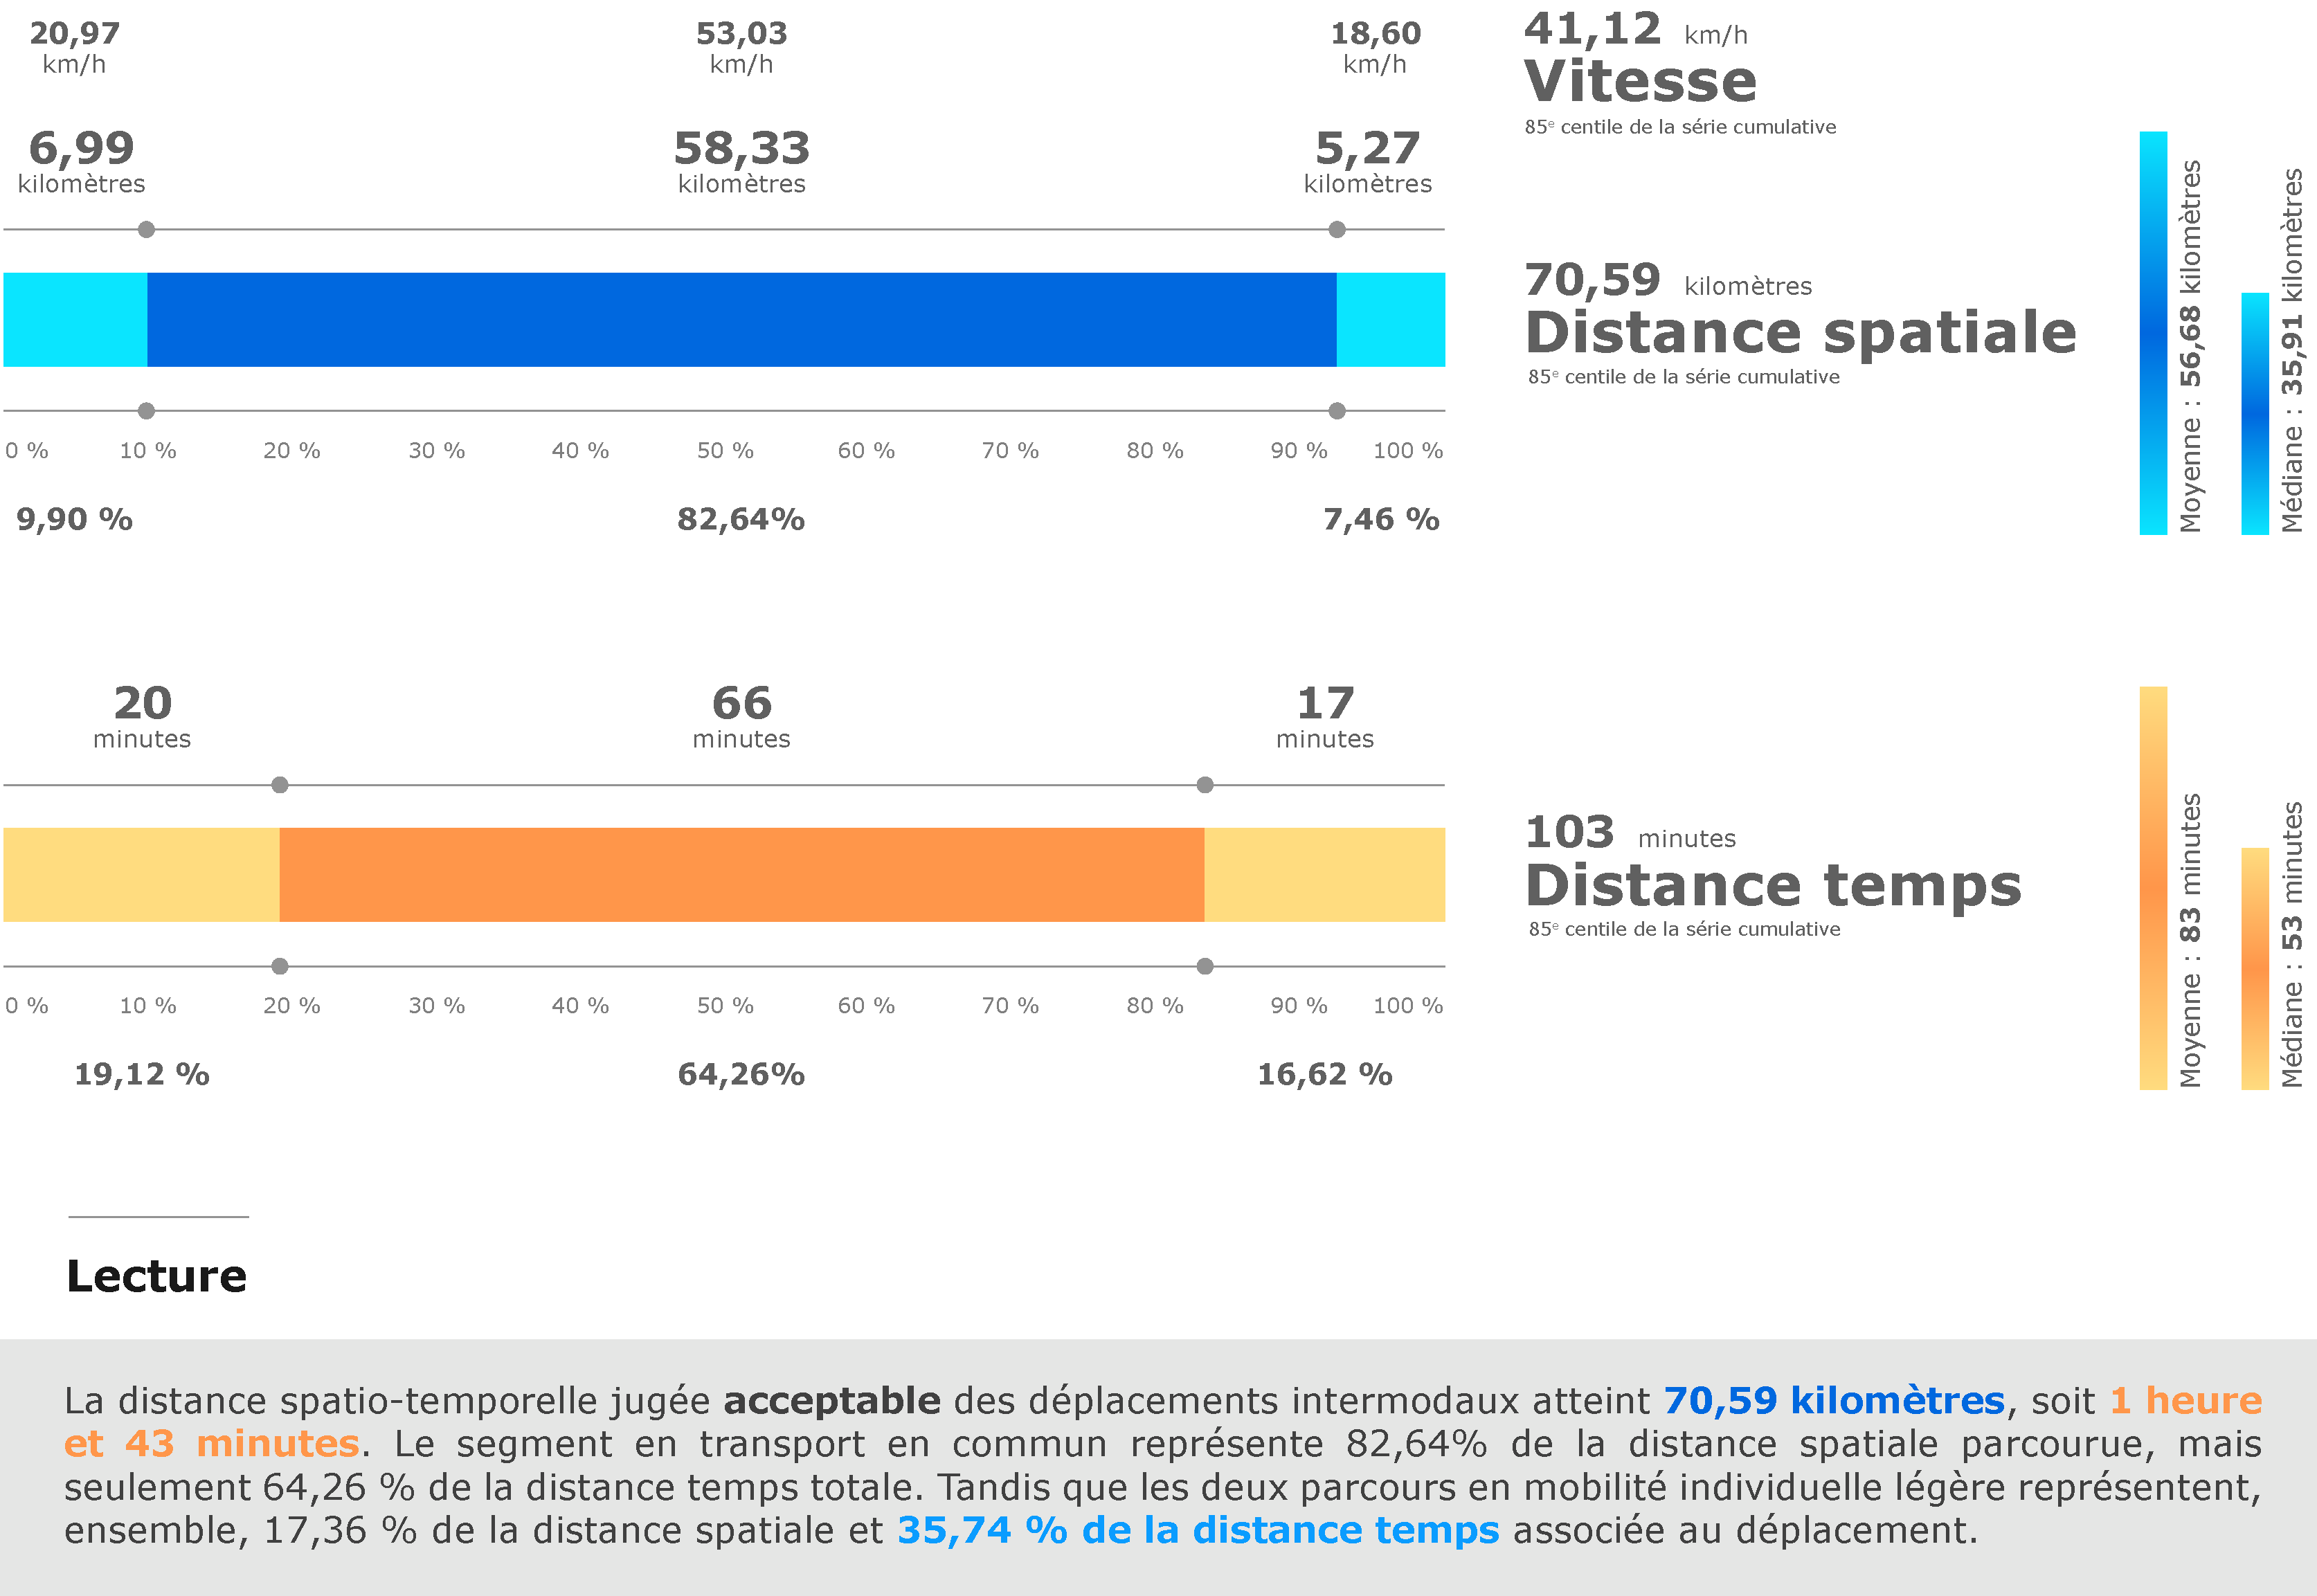
\includegraphics[width=1\columnwidth]{src/Figures/Chap-5/FR_Distances_Globales.pdf}}
        \vspace{5pt}
        \begin{flushleft}\scriptsize{
        \textcolor{blue}{Note~:} le calcul des distances-temps ne prend pas en considération le temps de précaution en arrivant en gare d'origine.
        }\end{flushleft}
        \begin{flushright}\scriptsize{
        Auteur~: \textcolor{blue}{Dylan Moinse (2024)}
        }\end{flushright}
    \end{figure}

    % Portée de la mobilité individuelle légère et des TC
Si la distance spatiale des déplacements intermodaux réalisés à l'aide de la mobilité individuelle légère atteint, en général, 70,59 kilomètres pour le 85\textsuperscript{e} centile de la série cumulative, les trois segments qui composent cette chaîne modale ne contribuent pas de manière équivalente à la distance totale parcourue (voir le \hyperref[fig-chap5:distances-globales]{diagramme~\ref{fig-chap5:distances-globales}}, page~\pageref{fig-chap5:distances-globales}). Comme attendu, le trajet en transport en commun représente en moyenne 82,64~\% de la distance spatiale totale parcourue. Parmi les 17,36~\% restants, effectués à vélo ou en micro-mobilité, le trajet en rabattement constitue 9,90~\% de la distance totale, tandis que le trajet en diffusion en représente 7,46~\%. En termes de distance-temps, la part moyenne du temps passé en transport en commun diminue à 64,26~\% de la durée moyenne en mouvement. Parmi les 35,74~\% de distance-temps consacrés à la mobilité individuelle légère, 19,12~\% du temps est alloué à l'étape en pré-acheminement et 16,62~\% à l'étape en post-acheminement. Ces données nous éclairent alors sur les ratios d'interconnectivité de la mobilité individuelle légère associée au transport public~–~dont la formule s'appuie sur la division de la distance de chaque segment par la distance globale du déplacement~–~de l'ordre de 0,17 en termes de distance spatiale et de 0,36 pour la dimension temporelle. Enfin, en termes de vitesse de déplacement, celle-ci atteint 40,97 kilomètres heure en moyenne, une vitesse plus faible que la vitesse moyenne de 51,30 kilomètres heure observée chez les automobilistes en France\footnote{
    Toutefois, il convient de nuancer cette comparaison, car la vitesse moyenne en automobile ne tient pas compte du temps nécessaire pour accéder au véhicule ni du temps de stationnement à destination. Nous pourrions ainsi supposer que la différence réelle entre les deux vitesses est bien moins significative qu'il n'y paraît initialement.
} \textcolor{blue}{\autocite{onisr_observatoire_2022}}\index{ONISR@\textsl{ONISR}|pagebf}.%%Rédigé%%

    % Comparaison enquêtes publiques
La distance totale parcourue, pour les navettes domicile-travail et domicile-études, en combinant l'usage de la mobilité individuelle légère et le réseau de transport en commun, atteint ainsi une moyenne de 56,68 kilomètres ou de 1 heure et 22 minutes. Cette distance est nettement supérieure à la distance spatiale moyenne parcourue par les habitant·e·s de la région Hauts-de-France en 2016, qui s'élève à 22,9 kilomètres ou 28 minutes pour rejoindre leur lieu de travail \textcolor{blue}{\autocite{insee_premiere_2016}}\index{Insee@\textsl{Insee}|pagebf}. En réalité, les résultats statistiques des déplacements analysés dans le cadre du questionnaire en ligne se rapprochent des distances observées par l'\textcolor{blue}{\textcite{insee_premiere_2016}}\index{Insee@\textsl{Insee}|pagebf} concernant la mobilité professionnelle ayant lieu depuis la région et en direction de la région francilienne, atteignant 57,7 kilomètres pour 1 heure et 5 minutes. En concentrant notre attention sur les flux en transport en commun, les distances mesurées dans notre étude~–~58 minutes en transport en commun~–~convergent peu ou prou vers l'enquête publique menée par le \textcolor{blue}{\textcite{ministere_de_la_transition_ecologique_et_de_la_cohesion_des_territoires_mobilite_2023}}\index{Ministère de la Transition Écologique et de la Cohésion des Territoires@\textsl{Ministère de la Transition Écologique et de la Cohésion des Territoires}|pagebf} qui indique qu'un déplacement \Guillemets{local ou longue distance}, réalisé en France, dure en moyenne 41 minutes en 2019.%%Rédigé%%

    % Comparaison littérature scientifique
Dans le cadre de cette recherche doctorale, nous avons exploré la portée globale des déplacements intermodaux, révélant une distance spatiale supérieure à celle documentée dans la littérature scientifique existante. Notre analyse secondaire d'une enquête menée par \textsl{SNCF Réseau} a permis de déterminer que la distance moyenne parcourue par les utilisateur·rice·s de la \acrshort{TEP} en association avec le \acrshort{TER} s'établit à 40,50 kilomètres, dans la région Provence-Alpes-Côte d'Azur. Bien que \textcolor{blue}{\textcite[8]{edel_potential_2021}}\index{Edel, Fabian|pagebf}\index{Wassmer, Simon|pagebf}\index{Kern, Mira|pagebf} observent que 44~\% des déplacements pendulaires en \acrshort{TEP} et combinés à l'usage du transport public dépassent 20 kilomètres, notre analyse statistique contraste avec les distances présentées dans certains travaux de recherche. À titre de comparaison, \textcolor{blue}{\textcite[7]{rabaud_micromobilites_2019}}\index{Rabaud, Mathieu|pagebf}\index{Richer, Cyprien|pagebf} rapportent une distance moyenne de déplacements intermodaux intégrant respectivement le vélo, le \acrshort{VLS} et la \acrshort{TEP} de 27,50~; 32,30 et 22,60 kilomètres en France. En association avec le \acrshort{TER} ou le \acrshort{RER}, \textcolor{blue}{\textcite[16]{gioria_etude_2016}}\index{Gioria, Christian|pagebf} mesure une distance spatiale moyenne de 39,50 kilomètres par les cyclistes en France, avec des écarts importants au profit des plus petites agglomérations. Par ailleurs, nos observations ne s'alignent pas sur les distances globales relatives à la combinaison du vélo et du rail, à hauteur de 53 kilomètres et de 41 kilomètres aux Pays-Bas \textcolor{blue}{\autocites[14]{shelat_analysing_2018}[225]{keijer_how_2000}}\index{Shelat, Sanmay|pagebf}\index{Huisman, Raymond|pagebf}\index{Oort, Niels van|pagebf}\index{Keijer, Majanka|pagebf}\index{Rietveld, Piet|pagebf} ou encore de 35 kilomètres en Belgique et en Angleterre \textcolor{blue}{\autocite[20 ; 28]{bitibi_bike_2017}}\index{BiTiBi@\textsl{BiTiBi}|pagebf}. Les valeurs que nous avons obtenues peuvent cependant entrer en résonance avec le travail de \textcolor{blue}{\textcite[116]{nigro_land_2019}}\index{Nigro, Antonio|pagebf}\index{Bertolini, Luca|pagebf}\index{Moccia, Francesco Domenico|pagebf} qui ont déduit une distance-temps totale d'un voyage pendulaire en train, en Italie, de 54 minutes. De plus, la place occupée par la mobilité individuelle légère au sein des déplacements intermodaux s'avère relativement similaire aux résultats de leur recherche, dans laquelle ces derniers ont estimé une durée respective en rabattement et en diffusion de 12 minutes, à l'aide du ratio d'interconnectivité développé par \textcolor{blue}{\textcite[274]{krygsman_multimodal_2004}}\index{Krygsman, Stephan|pagebf}\index{Dijst, Martin|pagebf}\index{Arentze, Theo|pagebf}\footnote{
    D'après \textcolor{blue}{\textcite[274]{krygsman_multimodal_2004}}\index{Krygsman, Stephan|pagebf}\index{Dijst, Martin|pagebf}\index{Arentze, Theo|pagebf} qui ont mesuré le temps de pré-acheminement et de post-acheminement généralement dépensé lors des déplacements intermodaux, y compris ceux intégrant l'usage du vélo, le ratio d'interconnectivité a une valeur moyenne comprise entre 0,20 et 0,50. Partant de ces données, \textcolor{blue}{\textcite[116]{nigro_land_2019}}\index{Nigro, Antonio|pagebf}\index{Bertolini, Luca|pagebf}\index{Moccia, Francesco Domenico|pagebf} ont retenu un seuil de 0,45 pour les deux segments réalisés à vélo.
}~; mais également au rapport d'étude du projet de recherche européen \textcolor{blue}{\textcite[20 ; 28]{bitibi_bike_2017}}\index{BiTiBi@\textsl{BiTiBi}|pagebf}, qui fait état d'une proportion égale à 11,43~\%, soit 4 kilomètres. De surcroît, la distance de 8,93 kilomètres ou de 24 minutes en métro, en tramway et en bus est corroborée par le temps de déplacement moyen de 12,50 kilomètres ou de 29 minutes observé à Séoul et à Daejeon, en Corée du Sud, comme le rapportent \textcolor{blue}{\textcite[46]{lee_strategies_2010}}\index{Lee, Jaeyeong|pagebf}\index{Shin, Hee-Cheol|pagebf}. L'écart notable entre le corpus restreint de la littérature scientifique et nos résultats statistiques peut alors être attribué à une surreprésentation des déplacements en \acrshort{TGV}, dans notre enquête, notamment entre Lille et Paris.%%Rédigé%%

    % 5.1.1.4.
    \needspace{1\baselineskip} % Réserve de l'espace
\subsubsection*{Détermination de la taille de l'\Guillemets{aire secondaire} des quartiers TOD
    \label{chap5:taille-aire-secondaire}
    }

    % Portée distance euclidienne
L'analyse des déplacements, associant l'usage du vélo ou de la micro-mobilité avec les transports en commun, indique que les \Guillemets{premiers et derniers kilomètres}~couvrent typiquement des distances individuelles oscillant entre trois et quatre kilomètres, en fonction du type de véhicule mobilisé. En approfondissant cette analyse à partir d'un plan euclidien, l'étape suivante consiste à délimiter la taille des quartiers \acrshort{TOD}, en prenant en compte leur extension facilitée par l'utilisation de la mobilité individuelle légère. En guise d'illustration, nous avons cartographié les abords de deux gares qui ont bénéficié d'un nombre important de réponses au sein de notre questionnaire~: la gare Lille Flandres, située dans le Nord, et la gare de Béthune, dans le Pas-de-Calais, toutes deux desservies par les réseaux \acrshort{TGV} et \acrshort{TER} (voir la \hyperref[fig-chap5:itineraires-lille-flandres]{carte~\ref{fig-chap5:itineraires-lille-flandres}}, page~\pageref{fig-chap5:itineraires-lille-flandres} et la \hyperref[fig-chap5:itineraires-bethune]{carte~\ref{fig-chap5:itineraires-bethune}}, page~\pageref{fig-chap5:itineraires-bethune}). Les cartographies des flux et des itinéraires démontrent que la mobilité individuelle légère complète plutôt qu'elle ne concurrence la marche, avec des distances minimales à vol d'oiseau d'environ 800 mètres. L'analyse révèle également que la majorité des déplacements s'effectue sur des distances euclidiennes de 1 à 2 kilomètres, souvent en partance du domicile. Pour la gare lilloise, il est intéressant de noter que les trajets en rabattement proviennent principalement de quartiers résidentiels situés à l'est (Fives, Saint-Maurice Pellevoisin et Marbrerie) et au sud (Gambetta et Wazemmes) des communes de Lille, Hellemmes et Ronchin, tandis que les trajets en diffusion se dirigent majoritairement vers les quartiers centraux, ce qui explique en partie la variation observée des distances (voir la \hyperref[fig-chap5:itineraires-lille-flandres]{carte~\ref{fig-chap5:itineraires-lille-flandres}}, page~\pageref{fig-chap5:itineraires-lille-flandres}). De façon similaire, autour de la gare béthunoise, les premiers kilomètres sont originaires des communes avoisinantes telles que Nœux-les-Mines, Barlin ou Busnes, alors que les derniers kilomètres se dirigent davantage vers les pôles d'activité en centre urbain et dans le secteur du centre hospitalier de Beuvry (voir la \hyperref[fig-chap5:itineraires-bethune]{carte~\ref{fig-chap5:itineraires-bethune}}, page~\pageref{fig-chap5:itineraires-bethune}). Ce résultat peut être interprété sous deux angles complémentaires. D'une part, il traduit une répartition plus diffuse des lieux de résidence et une concentration plus importante des emplois dans le quartier de gare. D'autre part, il reflète, dans un même contexte territorial et pour une même gare, des dynamiques de mobilité différentes selon qu'il s'agit d'un trajet en pré-acheminement ou en post-acheminement.%%Rédigé%%

    % Figure trajets autour de Lille Flandres
    \begin{carte}[h!]\vspace*{4pt}
        \caption{Cartographie des flux et des itinéraires suivis par les cyclo-voyageur·se·s se rendant ou en provenance de la gare Lille Flandres.}
        \label{fig-chap5:itineraires-lille-flandres}
        \centerline{\includegraphics[width=1\columnwidth]{src/Figures/Chap-5/FR_Distances_Itineraires_Lille_Flandres.png}}
        \vspace{5pt}
        \begin{flushright}\scriptsize{
        Auteur~: \textcolor{blue}{Dylan Moinse (2024)}
        }\end{flushright}
    \end{carte}

    % Figure trajets autour de Béthune
    \begin{carte}[h!]\vspace*{4pt}
        \caption{Cartographie des flux et des itinéraires suivis par les cyclo-voyageur·se·s se rendant ou en provenance de la gare de Béthune.}
        \label{fig-chap5:itineraires-bethune}
        \centerline{\includegraphics[width=1\columnwidth]{src/Figures/Chap-5/FR_Distances_Itineraires_Bethune.png}}
        \vspace{5pt}
        \begin{flushright}\scriptsize{
        Auteur~: \textcolor{blue}{Dylan Moinse (2024)}
        }\end{flushright}
    \end{carte}

    % Equivalent superficie
Partant de l'observation que le rayon d'un quartier de gare accessible à pied est typiquement d'un kilomètre, tandis que celui accessible par des modes cyclables s'étend de trois à quatre kilomètres, cette thèse met en lumière que les distances spatiales et temporelles parcourues à vélo ou en micro-mobilité sont trois à quatre fois plus importantes que celles réalisées à pied. Néanmoins, c'est en considérant la superficie des zones d'influence que le contraste devient particulièrement frappant. En effet, en calculant la surface de ces zones~–~la formule de l'aire d'un cercle consiste à multiplier le rayon au carré \(r^2\) par \(\pi\)~–, l'aire d'influence cyclable se révèle nettement plus étendue. Pour un quartier de gare accessible en mobilité individuelle légère avec un rayon de 3,8 kilomètres, la surface atteint 45,4 kilomètres carrés (avec une circonférence de 23,9 kilomètres), contre une aire de 5,3 kilomètres carrés (avec une circonférence de 8,2 kilomètres) pour une portée à pied à hauteur de 1,3 kilomètre. Cela revient à considérer que la mobilité individuelle légère permet d'augmenter l'accessibilité locale autour des nœuds de transport en commun de façon considérable, multipliant par 8,54 fois la taille de la zone accessible à pied.%%Rédigé%%

    % Éclater la bulle
Ajoutons que la taille du périmètre piétonnier établie à l'aide des réponses au questionnaire dépasse celle généralement observée dans les travaux académiques, les documents d'urbanisme et dans les études opérationnelles, où la limite spatiale pour les déplacements à pied, tant en rabattement qu'en diffusion, est habituellement fixée entre 500 et 800 mètres \textcolor{blue}{\autocite[133]{pojani_transit-oriented_2015}}\index{Pojani, Dorina|pagebf}\index{Stead, Dominic|pagebf}. La délimitation d'une accessibilité pédestre jusqu'à 1,3 kilomètre illustre l'extension de l'idée d'\Guillemets{éclatement de la bulle} (\Guillemets{\textsl{bursting the bubble}}), expression empruntée à \textcolor{blue}{Brian} \textcolor{blue}{\textcite[34]{canepa_bursting_2007}}\index{Canepa, Brian|pagebf}, Chef de projet au sein du cabinet d'étude \textsl{W-Trans}. Au travers de son article scientifique intitulé \textsl{Bursting the Bubble. Determining the Transit-Oriented Development’s Walkable Limits}, ce dernier invite les chercheur·se·s et les praticien·ne·s à remettre en question l'orthodoxie d'une limite pédestre de 500 mètres autour des quartiers \acrshort{TOD}. La redéfinition de cette limite est corroborée par la revue de littérature produite par \textcolor{blue}{Alain} \textcolor{blue}{\textcite[5]{lhostis_perimetres_2016}}\index{L'Hostis, Alain|pagebf}, qui conteste la pertinence de la barrière arbitraire des 800 mètres, équivalente à la règle des 0,5 mile, et préconise son extension, une position également soutenue par \textcolor{blue}{\textcite[79]{ker_myths_2003}}\index{Ker, Ian|pagebf}\index{Ginn, Simon|pagebf} qui qualifient cette limite de mythe ou de dogme. En conséquence, notre recherche participe à la déconstruction de cette bulle préconçue à deux niveaux distincts~: l'aire des quartiers \acrshort{TOD} passe de 2,01 kilomètres carrés (pour un rayon de 0,8 kilomètre) à 5,31 kilomètres carrés (pour 1,3 kilomètre) en ce qui concerne la marche, et s'étend jusqu'à 45,36 kilomètres carrés (pour 3,8 kilomètres) pour le vélo et la micro-mobilité. Ainsi, la détermination d'un quartier de gare fondé sur les pratiques de mobilité déclarées nous amène à envisager une zone accessible jusqu'à 2,64 fois plus grande pour la marche et 22,57 fois plus vaste grâce à la mobilité individuelle légère.%%Rédigé%%

    % Figure aires d'influence
    \begin{carte}[h!]\vspace*{4pt}
        \caption{Superficie occupée par l'extension des quartiers de gare piétonniers et cyclables, à l'échelle de la région Hauts-de-France.}
        \label{fig-chap5:aires-influence}
        \centerline{\includegraphics[width=1\columnwidth]{src/Figures/Chap-5/FR_Distances_Aires_influence_compressed.pdf}}
        \vspace{5pt}
        \begin{flushright}\scriptsize{
        Auteur~: \textcolor{blue}{Dylan Moinse (2024)}
        }\end{flushright}
    \end{carte}
    
    % Aires d'influence
En extrapolant ce seuil de distance estimé à l'échelle des 318 gares actuellement exploitées dans la région Hauts-de-France, cette recherche avance que la marche combinée offre un accès à 3,06~\% de la superficie du territoire à vol d'oiseau, et à 0,94~\% du territoire en prenant en compte l'infrastructure piétonne existante (voir la \hyperref[fig-chap5:impedance-distances]{carte~\ref{fig-chap5:aires-influence}}, page~\pageref{fig-chap5:aires-influence}). L'introduction de la mobilité individuelle légère hisse l'accessibilité territoriale à 21,54~\% de la région à vol d'oiseau, et à 7,55~\% en considérant le réseau viaire accessible à vélo (voir la \hyperref[fig-chap5:impedance-distances]{carte~\ref{fig-chap5:aires-influence}}, page~\pageref{fig-chap5:aires-influence}). Cependant, les disparités entre les zones tampons et les isodistances nous éclairent également sur la compression du potentiel d'accessibilité en raison de la présence de barrières physiques et du tissu urbain, qui tendent à réduire l'accessibilité piétonne réelle par un facteur de 3,26 et l'accessibilité cyclable par un facteur de 2,85. Au-delà de cette discussion sur les surfaces accessibles, nous allons voir quels sont les aspects qui influent le plus dans la variabilité des distances établies.%%Rédigé%%

    % 5.1.2.
    \needspace{1\baselineskip} % Réserve de l'espace
\subsection{Influence des caractéristiques urbaines et individuelles sur les distances spatiales parcourues
    \label{chap5:regression-distances}
    }

    % Objectif
Après avoir établi les seuils de distance spatiale et temporelle considérés comme acceptables par les usager·ère·s, notre recherche s'est orientée vers l'analyse de l'impact de divers facteurs liés aux caractéristiques des territoires traversés, aux comportements et aux habitudes de mobilité des voyageur·se·s intermodaux·les, ainsi qu'à leur profil socio-démographique sur la variabilité des distances estimées. Pour ce faire, nous avons employé la méthode de régression des moindres carrés ordinaires (\textsl{Ordinary Least Squares}, OLS), une technique statistique reconnue pour son efficacité à estimer les relations entre une variable dépendante~–~en l'occurrence, la distance~–~et plusieurs variables indépendantes. Cette méthode a pour avantage de minimiser la somme des carrés des résidus, c'est-à-dire des écarts entre les valeurs observées et celles prédites par le modèle de régression multiple, qui se révèle être le mieux ajusté aux données collectées.%%Rédigé%%

    % 5.1.2.1.
    \needspace{1\baselineskip} % Réserve de l'espace
\subsubsection*{Application d'un modèle de régression linéaire couplé à un modèle à élasticité constante
    \label{chap5:modeles-OLS-log-log}
    }

    % Méthodologie OLS
L'application de cette régression nous permet de déterminer les coefficients de détermination, notés R\textsuperscript{2} et R\textsuperscript{2} ajusté. Le R\textsuperscript{2} indique la proportion de la variance totale de la variable dépendante qui est expliquée par les variables indépendantes du modèle. Toutefois, compte tenu de la présence d'un nombre conséquent de prédicteurs dans notre modèle, susceptibles d'influer artificiellement sur le R\textsuperscript{2}, nous accordons une importance particulière au R\textsuperscript{2} ajusté. Ce dernier, en effet, a la particularité de réduire la valeur du R\textsuperscript{2} lorsque l'ajout de variables supplémentaires au modèle ne contribue pas de manière significative à améliorer la capacité du modèle à expliquer la variance observée, pénalisant ainsi l'inclusion de variables superflues.%%Rédigé%%

    % Modélisation Log-log
En sus de la régression des moindres carrés ordinaires, une approche de modélisation log-log, également désignée sous le terme de modèle à double logarithme ou de modèle à élasticité constante, a été mise en œuvre. Cette méthode vise à estimer les élasticités, c'est-à-dire la sensibilité proportionnelle de la variable dépendante, ici la distance, aux variations des variables indépendantes. Ce type de modèle offre une approche analytique distincte qui enrichit la compréhension des interactions entre les variables en mesurant les effets de manière proportionnelle au moyen du coefficient de détermination \(\beta\). Cette perspective particulière permet ainsi une appréciation des effets proportionnels calculés des variables indépendantes sur la variable dépendante.%%Rédigé%%

    % Facteurs interrogés
Dans le cadre de ce modèle statistique, les deux régressions se sont appuyées sur une gamme de variables indépendantes, extraites à la fois du questionnaire distribué aux usager·ère·s et de l'analyse statistique et spatiale qui en découle. Ces variables sont énumérées ci-dessous~:
\begin{customitemize}
    \item Le type de mode de transfert impliqué~;
    \item Les modalités d'embarquement ou le type de stationnement adopté pour le véhicule~;
    \item Le système de transport en commun~;
    \item L'effet de substitution modale~;
    \item La distance-temps du trajet en rabattement ou en diffusion~;
    \item La densité démographique aux abords des points d'origine ou de destination~;
    \item Le relief du terrain traversé~;
    \item Le niveau de confort ressenti de l'itinéraire en rabattement et en diffusion~;
    \item Le motif de déplacement~;
    \item La fréquence d'usage~;
    \item L'expérience intermodale des usager·ère·s~;
    \item Les habitudes de mobilité des usager·ère·s~;
    \item La composition du foyer~;
    \item La possession de vélos au sein du ménage~;
    \item Le taux de motorisation du ménage~;
    \item Le genre des usager·ère·s~;
    \item L'âge des usager·ère·s~;
    \item La situation professionnelle des usager·ère·s~;
    \item Le secteur d'activité professionnel des usager·ère·s~;
    \item Le niveau de diplôme des usager·ère·s~;
    \item Le revenu annuel disponible des usager·ère·s.
\end{customitemize}%%Rédigé%%

    % 5.1.2.2. 
    \needspace{1\baselineskip} % Réserve de l'espace
\subsubsection*{Déterminants des distances spatiales franchies
    \label{chap5:facteurs-modeles-OLS-log-log}
    }

    % Résultats généraux
Le coefficient de détermination global du modèle se situe à 0,90, tandis que le R\textsuperscript{2} ajusté atteint 0,79. Ce résultat indique que 90,20~\% de la variabilité de la variable dépendante est expliquée par les variables indépendantes intégrées dans le modèle. La présence d'un R\textsuperscript{2} ajusté sensiblement inférieur au R\textsuperscript{2} brut suggère que certaines variables incluses dans l'analyse ne contribuent pas de manière significative à l'explication de la variance observée dans la variable de distance. Afin de rectifier un éventuel surajustement, il est proposé de retirer du modèle des moindres carrés ordinaires certaines variables. Ces exclusions concernent les modalités d'embarquement ou le type de stationnement adopté pour le véhicule, les effets de substitution modale, à l'exception de ceux impliquant l'usage de la voiture, les habitudes de mobilité autres que la marche, ainsi que les variables liées à l'équipement en vélos et en voitures, à l'âge, à la situation professionnelle, au niveau de diplôme et au revenu disponible des voyageur·se·s.%%Rédigé%%

    % Tableau corrélation facteurs
% Tableau corrélation facteurs
%%Rédigé%%
    \begin{table}[h!]
    \centering
    \renewcommand{\arraystretch}{1.5}
    \resizebox{\columnwidth}{!}{
    \begin{tabular}{p{0.46\columnwidth}p{0.14\columnwidth}p{0.16\columnwidth}p{0.11\columnwidth}p{0.13\columnwidth}}
        %\hline
    \rule{0pt}{15pt} \multirow{1.5}{*}{\small{\textbf{\textcolor{blue}{Variables indépendantes}}}} & \small{\textbf{\textcolor{blue}{Élasticité \(\beta\)}}} & \small{\textbf{\textcolor{blue}{Coefficient R\textsuperscript{2}}}} & \small{\textbf{\textcolor{blue}{P-valeur}}} & \multirow{1.5}{*}{\textbf{\textcolor{blue}{$\sigma$}}}\\
        \hline
\small{Type de mobilité individuelle légère} & \small{\textbf{1,54~\%}} & \small{1~815,23} & \small{0,13} & \small{1~413,59}\\
\small{Temps de déplacement**} & \small{\textbf{1,21~\%}} & \small{286,51} & \small{0,00} & \small{8,87}\\
\small{Fréquence d'utilisation**} & \small{\textbf{0,73~\%}} & \small{652,86} & \small{0,01} & \small{479,09}\\
\small{Professions (\acrshort{PCS})*} & \small{\multirow{1.5}{*}{\textbf{0,64~\%}}} & \small{\multirow{1.5}{*}{196,93}} & \small{\multirow{1.5}{*}{0,05}} & \small{\multirow{1.5}{*}{994,67}}\\
\small{Taille du ménage*} & \small{\textbf{0,54~\%}} & \small{2~166,65} & \small{0,05} & \small{1~110,77}\\
\small{Système de transport en commun**} & \small{\textbf{0,46~\%}} & \small{1~262,87} & \small{0,00} & \small{393,99}\\
\small{Substitution de la voiture} & \small{\textbf{0,40~\%}} & \small{616,49} & \small{0,23} & \small{516,99}\\
\small{Motif de déplacement} & \small{\textbf{0,28~\%}} & \small{491,88} & \small{0,25} & \small{430,49}\\
\small{Genre} & \small{\textbf{0,17~\%}} & \small{-279,85} & \small{0,28} & \small{609,83}\\
\small{densité de population} & \small{\textbf{-0,01~\%}} & \small{-0,02} & \small{0,16} & \small{0,01}\\
\small{Sensation de confort} & \small{\textbf{-0,13~\%}} & \small{-40,41} & \small{0,15} & \small{82,90}\\
\small{Dénivelé du terrain**} & \small{\textbf{-0,13~\%}} & \small{-5,81} & \small{0,04} & \small{2,77}\\
\small{Expérience intermodale} & \small{\textbf{-0,23~\%}} & \small{-357,81} & \small{0,45} & \small{752,37}\\
\small{Pratique fréquente de la marche**} & \small{\textbf{-0,32~\%}} & \small{-284,01} & \small{0,01} & \small{109,53}\\
        \hline
        \end{tabular}}
    \caption{Statistiques descriptives du modèle à élasticité constante mesurant les effets proportionnels des variables indépendantes sur la distance spatiale en mobilité individuelle légère.}
    \label{table-chap5:facteurs-distance-spatiale}
        \vspace{5pt}
        \begin{flushleft}\scriptsize{
        \textcolor{blue}{Lecture~:} toutes choses égales par ailleurs, lorsqu'une variable indépendante augmente de 1~\%, la valeur de la distance augmente à son tour de $X$~\%.
        \\
        \textcolor{blue}{Note~:} **$p$~\textless~0,05, *$p$~\textless~0,10, $\sigma$~correspond à l'écart-type.
        }\end{flushleft}
        \begin{flushright}\scriptsize
        Auteur~: \textcolor{blue}{Dylan Moinse (2023)}
        \end{flushright}
        \end{table}%%Rédigé%%

    % Résultats influence positive et négative
L'analyse de l'élasticité dans le cadre du modèle de régression révèle que les variables exerçant une influence prépondérante sur la distance spatiale parcourue par les utilisateur·rice·s de la mobilité individuelle légère et du transport public incluent principalement la forme de la combinaison modale, la durée des trajets, la fréquence d'utilisation, les \acrfull{PCS}, la composition du ménage, la substitution de l'automobile, la régularité de la marche, ainsi que le motif de déplacement (voir le \hyperref[table-chap5:facteurs-distance-spatiale]{tableau~\ref{table-chap5:facteurs-distance-spatiale}}, page~\pageref{table-chap5:facteurs-distance-spatiale}). En maintenant constantes les autres variables, il apparaît que si la distance-temps augmente de 1~\%, la distance spatiale correspondante s'accroît de 1,21~\%. De même, une augmentation de 1~\% de la fréquence d'utilisation se traduit par un accroissement de 0,73~\% de la distance parcourue. Concernant la combinaison modale, l'accroissement de 1~\% de la probabilité de l'utilisation du vélo entraîne une hausse de 1,54~\% de la distance parcourue, tandis que l'usage du \acrshort{TGV} augmente la distance de 0,46~\%. Par ailleurs, l'analyse statistique montre que la distance spatiale connaît une variation positive lorsque l'usager·ère tend à être un·e cadre supérieur·e (0,64~\%) ou un homme (0,17~\%), que le foyer s'agrandit (0,54~\%) ou que le déplacement revêt un caractère utilitaire (0,28~\%). Inversement, toutes choses égales par ailleurs, la distance parcourue tend à diminuer de 0,32~\% lorsque l'usager·ère a pour habitude de marcher, et de 0,23~\% lorsque celui-ci a adopté des pratiques intermodales plus récemment.%%Rédigé%%

    % Résultats pas d'influence notable
Ces observations soulignent les éléments influant sur la distance spatiale des trajets, illustrant l'impact des choix modaux, des habitudes de déplacement, ainsi que des caractéristiques individuelles sur l'étendue des parcours. La régression présentée dans le \hyperref[table-chap5:facteurs-distance-spatiale]{tableau~\ref{table-chap5:facteurs-distance-spatiale}} (page~\pageref{table-chap5:facteurs-distance-spatiale}) démontre également que certains facteurs ont un impact négligeable sur cette relation, comme le montre la densité de population (0,01~\%), ou mineur, tel que l'évaluation subjective de la qualité des itinéraires (-0,13~\%) ou le dénivelé du terrain (-0,13~\%). Ces résultats statistiques suivent la recherche menée par \textcolor{blue}{\textcite[181]{gan_associations_2021}}\index{Gan, Zuoxian|pagebf}\index{Yang, Min|pagebf}\index{Zeng, Qingcheng|pagebf}\index{Timmermans, Harry~J.~P.|pagebf} à Nanjing, qui n'a pas établi de lien significatif entre la densité démographique et la distance parcourue à vélo autour des stations de métro. Si l'impact négatif des pentes sur le rapport des usager·ère·s à la distance n'est pas surprenant, l'effet négatif de la sensation de confort pourrait sembler contre-intuitif. Toutefois, il est plausible que la notation de la qualité des parcours rapportée par les voyageur·se·s diminue précisément parce que des distances plus longues impliquent souvent des itinéraires plus complexes et généralement situés hors des centres urbains. Cette hypothèse a aussi été discutée par \textcolor{blue}{\textcite[185]{gan_associations_2021}}\index{Gan, Zuoxian|pagebf}\index{Yang, Min|pagebf}\index{Zeng, Qingcheng|pagebf}\index{Timmermans, Harry~J.~P.|pagebf}, qui ont également découvert que l'expérience de confort à vélo est négativement corrélée aux distances franchies, suggérant que l'environnement urbain traversé par des trajets plus longs tendent à être évalués plus négativement.%%Rédigé%%

    % Résultats access VS egress
En distinguant, au sein du modèle de régression, les trajets effectués depuis le domicile de ceux dirigés vers le lieu d'activité, des nuances dans les effets de certains facteurs émergent. Bien que l'influence de la durée de déplacement sur la distance spatiale demeure constante (1,25~\% en rabattement et 1,18~\% en diffusion), l'impact de la substitution modale au détriment de l'usage de la voiture varie notablement. Ainsi, en phase de pré-acheminement, l'élasticité atteint 0,60~\% pour les ancien·ne·s conducteur·rice·s et 0,50~\% pour les ancien·ne·s passager·ère·s, tandis qu'en post-acheminement, ces valeurs s'inversent respectivement à -0,28~\% et -0,31~\%. Cet écart manifeste peut s'expliquer en partie par le fait que les trajets en rabattement, initialement réalisés par le biais de l'automobile, sont généralement plus longs que ceux effectués vers le lieu d'activité. Un second élément notable concerne l'asymétrie de l'impact de la taille du ménage qui se manifeste différemment selon les segments du déplacement intermodal~: les ménages constitués d'un ou de deux parents avec un ou plusieurs enfants tendent à être moins sensibles face à un allongement des distances en rabattement (élasticité de la demande de 0,62~\% et de 0,33~\%), tandis qu'un effet inverse est constaté en phase de diffusion (élasticité de -0,30~\% et de -0,38~\%) en comparaison avec les ménages sans enfant. Cette dynamique suggère l'existence d'une chaîne de déplacement réalisée en amont du trajet principal en transport en commun, principalement pour l'accompagnement des enfants. Les réponses au questionnaire, notamment à la question \Guillemets{\textsl{Avez-vous effectué un arrêt intermédiaire lors de votre trajet [en rabattement et, ou bien, en diffusion]~?}}, où 37 participant·e·s ont indiqué avoir effectué arrêt intermédiaire pour des motifs d'accompagnement, illustrent cette tendance. Parmi ces 37 répondant·e·s, 17 d'entre elleux font partie d'un ménage avec un ou plusieurs enfants (45,95~\%), une proportion supérieure à celle observée dans l'ensemble de la population ciblée par l'enquête, qui comprend 74 ménages avec enfants, représentant 33,94~\% de l'échantillon total.%%Rédigé%%

    % Transition
Cette analyse des distances parcourues lors des \Guillemets{premiers et derniers kilomètres} des systèmes de transport en commun met en lumière une diversité de pratiques intermodales influencées par des facteurs personnels et contextuels variés. De ce point de vue, nous sommes amenés à aborder la question suivante dans la prochaine sous-section~: quels sont les gains d'accessibilité à l'échelle régionale engendrés par l'usage intermodal de la mobilité individuelle légère~? Ce glissement d'une échelle locale à une perspective régionale nous permet de mieux comprendre comment l'extension des quartiers de gare est à même de remodeler l'accessibilité régionale.%%Rédigé%%
    
     % ___________________________________________
    % 5.2.
    \newpage
    \needspace{1\baselineskip} % Réserve de l'espace
    \sectionheader{Gains d'accessibilité régionale}
\section{Des gains d'accessibilité intermodale rendus possible par l’extension des aires d’influence autour des nœuds du réseau de transport en commun
    \label{chap5:accessibilite-intermodale-extension-aire-influence}
    }

    % Introduction
L'extension des aires d'influence autour des nœuds du réseau de transport en commun génère des gains considérables en termes d'\gls{accessibilité intermodale}, notamment grâce à l'intégration de la mobilité individuelle légère. L'essor des services intermodaux et des pratiques de mobilité qui en découlent requièrent une approche holistique de la performance territoriale du système de transport, allant au-delà d'une évaluation sectorielle. En effet, la seule mesure de la distance physique apparaît insuffisante, car elle ne tient pas compte de la dimension sociale de l'accessibilité, laquelle intègre un caractère contextuel et particulier \textcolor{blue}{\autocite[3]{lhostis_definir_2010}}\index{L'Hostis, Alain|pagebf}\index{Conesa, Alexis|pagebf}\index{Arnaud Banos, Thomas Thévenin|pagebf}. Il est donc impératif de revoir les méthodes d'évaluation de l'offre de transport et les calculs d'accessibilité, en prenant en compte la variété des combinaisons modales et leur efficacité relative \textcolor{blue}{\autocite[111]{chapelon_transports_2016}}\index{Chapelon, Laurent|pagebf}. À ce titre, nous examinons dans cette section comment cette extension, d'ordre spatial, peut améliorer l'accessibilité régionale eu égard au potentiel de report modal exprimé à travers l'accès de la population au système de mobilité, ainsi qu'aux emplois et aux \acrfull{POIs}, correspondant aux \textsl{Points of Interest} ou aux \Guillemets{sites utiles}. En abordant la question de l'accessibilité intermodale, cette analyse s'articule autour de plusieurs sous-sections, explorant successivement l'\hyperref[chap5:couverture-population]{amélioration du potentiel d'accès des gares par la population} (page~\pageref{chap5:couverture-population}) et les \hyperref[chap5:accessibilite-emplois]{gains d'accessibilité vers les zones d'emploi et vers les différents lieux d'attraction territoriale} (page~\pageref{chap5:accessibilite-emplois}).%%Rédigé%%

    % 5.2.1.
    \needspace{1\baselineskip} % Réserve de l'espace
\subsection{Amélioration du potentiel de couverture de la population par le système de transport en commun
    \label{chap5:couverture-population}
    }

    % Introduction
L'intégration de la mobilité individuelle légère au sein du réseau de transport en commun constitue un axe crucial pour l'évaluation d'un modèle \acrshort{TOD} revisité dans la région concernée. Dans cette sous-section, nous abordons les implications des gains d'accessibilité intermodale en termes de couverture géographique et démographique régionale, ainsi que le potentiel de report modal vers ce système de mobilité. À cet égard, nous examinons en premier lieu la part de la population desservie par l'élargissement des zones d'influence des gares. Puis, nous caractérisons la densité démographique de ces terrains et considérons les contours d'une accessibilité qui se veut plus inclusive.%%Rédigé%%

    % 5.2.1.1.
    \needspace{1\baselineskip} % Réserve de l'espace
\subsubsection*{Vers un triplement du potentiel de report modal vers le réseau de transport public régional
    \label{chap5:couverture-regionale}
    }
    
    % Gains d'accessibilité région
L'extension des quartiers de gare permise par l'essor de la mobilité individuelle légère suppose une amélioration de la desserte territoriale du système de transport en commun, à l'échelle régionale. Comme le montrent le \hyperref[table-chap5:couverture-spatiale]{tableau~\ref{table-chap5:couverture-spatiale}} (page~\pageref{table-chap5:couverture-spatiale}) ainsi que la \hyperref[fig-chap5:impedance-distances]{carte~\ref{fig-chap5:aires-influence}} (page~\pageref{fig-chap5:aires-influence}) présentée dans la \hyperref[chap5:taille-aire-secondaire]{section précédente} traitant de la détermination de la taille des quartiers de gare (page~\pageref{chap5:taille-aire-secondaire}), l'aire effectivement accessible à pied est multipliée par huit grâce à l'élargissement de la portée de la mobilité individuelle légère. Avec une superficie régionale de 31~936 kilomètres carrés, l'\Guillemets{aire primaire} réelle s'étend sur 302 kilomètres carrés, tandis que l'\Guillemets{aire secondaire} réelle couvre 2~110 kilomètres carrés, soit dans l'ensemble, une aire d'influence de 2~412 kilomètres carrés. En conséquence, la couverture régionale des quartiers \acrshort{TOD} passe de 0,94~\% à 7,55~\%, et détient un potentiel pouvant atteindre 18,48~\% (6~878 kilomètres carrés) de la région, en prenant en compte les effets de \gls{coupure urbaine} et les obstacles physiques.%%Rédigé%%

    % Accessibilité population
En examinant de plus près la couverture de la population à l'échelle régionale, il apparaît que les quartiers de gare accessibles à pied, en tenant compte du réseau viaire, couvrent 19,52~\% de la population des Hauts-de-France, soit 1~170~135 habitants. Par ailleurs, l'\Guillemets{aire secondaire} seule est capable de couvrir plus d'un tiers de la population régionale, représentant 36,18~\% des habitant·e·s, soit 2~169~229 personnes. Ainsi, les quartiers de gare accessibles à la fois aux piéton·ne·s et aux cyclistes permettent de couvrir plus de la moitié de la population régionale, équivalant à 55,70~\% ou 3~339~364 résident·e·s (voir le \hyperref[table-chap5:couverture-spatiale]{tableau~\ref{table-chap5:couverture-spatiale}}, page~\pageref{table-chap5:couverture-spatiale}). Sous cette perspective, le périmètre combiné des quartiers de gare, tant piétonniers que cyclables, s'étend à 8,03 fois celui limité à la portée piétonne et englobe 2,85 fois plus de résident·e·s bénéficiant d'un accès aux gares.%%Rédigé%%

    % Tableau couverture population régionale
% Tableau couverture population régionale
%%Rédigé%%
    \begin{table}[h!]
    \centering
    \renewcommand{\arraystretch}{1.5}
    \resizebox{\columnwidth}{!}{
    \begin{tabular}{p{0.33\columnwidth}p{0.12\columnwidth}p{0.12\columnwidth}p{0.15\columnwidth}p{0.13\columnwidth}p{0.15\columnwidth}}
        %\hline
    \rule{0pt}{15pt} \multirow{1.5}{*}{\small{\textbf{\textcolor{blue}{Périmètre géographique}}}} & \small{\textbf{\textcolor{blue}{Distances (km)}}} & \small{\textbf{\textcolor{blue}{Distances (min)}}} & \small{\textbf{\textcolor{blue}{Superficie Région (\%)}}}& \small{\textbf{\textcolor{blue}{Population (\%)}}} & \small{\textbf{\textcolor{blue}{Densité (hab/km\textsuperscript{2})}}}\\
        \hline
\small{Isochrones piétonnes} & \small{\textless1} & \small{\textless12} & \small{0,94} & \small{19,52} & \small{3~880,25}\\
\small{Aires piétonnes} & \small{\textless1} & \small{\textless12} & \small{3,06} & \small{25,27} & \small{1~552,20}\\
        \hdashline
\small{Isochrones cyclables} & \small{{[}1~;~4{[}} & \small{\textless12 } & \small{6,61} & \small{36,18} & \small{1~028,07}\\
\small{Aires cyclables} & \small{{[}1~;~4{[}} & \small{\textless12} & \small{18,48} & \small{40,13} & \small{407,68}\\
        \hdashline
\small{Isochrones piétonnes et cyclables} & \multirow{1.5}{*}{\small{\textless4}} & \multirow{1.5}{*}{\small{\textless12}} & \multirow{1.5}{*}{\small{7,55}} & \multirow{1.5}{*}{\small{55,70}} & \multirow{1.5}{*}{\small{1~384,73}}\\
\small{Aires piétonnes et cyclables} & \small{\textless4} & \small{\textless12} & \small{21,54} & \small{65,40} & \small{570,13}\\
        \hdashline
\small{Isochrones non accessibles} & \small{\Geq 4} & \small{\Geq 12} & \small{92,45} & \small{44,30} & \small{89,96}\\
\small{Aires non accessibles} & \small{\Geq 4} & \small{\Geq 12} & \small{78,46} & \small{34,60} & \small{82,77}\\
        \hline
        \end{tabular}}
    \caption{Couverture de la population régionale par le réseau ferroviaire soutenu par la mobilité individuelle légère.}
    \label{table-chap5:couverture-spatiale}
        \vspace{5pt}
        \begin{flushleft}\scriptsize{
        \textcolor{blue}{Note~:} la densité moyenne de la population de la région Hauts-de-France était de 189 hab/km\textsuperscript{2} en 2021.
        \\
        \textcolor{blue}{Lecture~:} contrairement aux aires d'influence des gares accessibles à pied, les quartiers de gare étendus par la mobilité individuelle légère couvrent une majeure partie de la population des Hauts-de-France. Cependant, un tiers de la population régionale n'a théoriquement pas accès aux gares, malgré l'usage du vélo ou de la micro-mobilité. Par ailleurs, plus des trois quarts du territoire administratif ne peut être couvert, amenant à nous questionner sur l'accès aux destinations telles que les emplois ou certaines aménités.
        }\end{flushleft}
        \begin{flushright}\scriptsize
        Jeux de données~: données carroyées de l'\textcolor{blue}{\textcite{insee_grille_2021}}\index{Insee@\textsl{Insee}|pagebf}
        \\
        Auteur~: \textcolor{blue}{Dylan Moinse (2023)}
        \end{flushright}
        \end{table}%%Rédigé%%

    % Densité démographique
Concernant la densité de population à l'échelle régionale, celle-ci tend à décroître à mesure que la distance depuis les gares de la région Hauts-de-France augmente. À cet effet, la densité démographique moyenne dans les quartiers de gare accessibles à pied est de 3~880 habitants par kilomètre carré, un chiffre qui surpasse de 3,77 fois celui enregistré dans les quartiers de gare accessibles à vélo ou en micro-mobilité, où l'accessibilité piétonne est exclue. Ce différentiel suggère potentiellement une préférence des citadin·e·s pour un environnement moins densément peuplé dans les \Guillemets{aires secondaires}, mais reflète également un déficit potentiel de stratégies d'aménagement urbain orientées sur le développement ferroviaire. Ainsi, cet écart met en exergue le besoin d'une intensification urbaine qui pourrait davantage concentrer la population autour d'un périmètre accessible autour des gares.%%Rédigé%%

    % Littérature
Notre recherche met en lumière les avantages substantiels de la combinaison de la mobilité individuelle légère avec le transport public en termes d'accessibilité aux populations vivant à proximité des gares de la région. Celle-ci démontre que l'extension des quartiers \acrshort{TOD} permet de connecter 2,85 fois plus d'individus comparativement aux périmètres piétons. Ces résultats s'associent à l'étude de \textcolor{blue}{\textcite[213]{kager_characterisation_2016}}\index{Kager, Roland|pagebf}\index{Bertolini, Luca|pagebf}\index{te Brömmelstroet, Marco|pagebf} qui considère que l'intégration du vélo conventionnel garantit une multiplication par quinze du nombre de Néerlandais·e·s ayant accès aux principales gares interurbaines et par quatre concernant les gares locales. De plus, l'usage intermodal du vélo assure la desserte de 69~\% de la population dans un rayon de cinq kilomètres, et de 81~\% jusqu'à 7,5 kilomètres, tandis que seulement 19~\% de la population a accès au système de transport en commun à pied  \textcolor{blue}{\autocite[213]{kager_characterisation_2016}}\index{Kager, Roland|pagebf}\index{Bertolini, Luca|pagebf}\index{te Brömmelstroet, Marco|pagebf}. Ces chiffres complètent également les recherches de \textcolor{blue}{\textcite[22]{marques_potential_2017}}\index{Marques,~R.|pagebf}\index{Lovelace, Robin|pagebf} qui démontrent qu'une extension de l'aire d'influence des stations de transport en commun à Séville permet d'inclure plus de 31~\% de la population métropolitaine, contre une couverture de 6~\% réalisée par la marche seule. Par ailleurs, l'étude de \textcolor{blue}{\textcite[982]{lee_bicycle-based_2016}}\index{Lee, Jaeyeong|pagebf}\index{Choi, Keechoo|pagebf}\index{Leem, Yountaik|pagebf} met en avant une couverture de 94~\% de la population à Séoul, comparativement à 30~\% pour la marche combinée, triplant ainsi l'accessibilité métropolitaine.%%Rédigé%%

    % 5.2.1.2.
    \needspace{1\baselineskip} % Réserve de l'espace
\subsubsection*{Interactions entre l'accessibilité de la population aux quartiers de gare et leur densité urbaine
    \label{chap5:analyse-bivariee-densite-accessibilite}
    }

    % Densité analyse bivariée
La question de l'accessibilité intermodale de la population régionale, croisée avec la densité de population, a été posée dans le but d'adopter une perspective globale sur ces deux indicateurs et de mieux comprendre les interactions existantes. Cette relation repose sur le niveau d'accessibilité basé sur le réseau ferroviaire, la marche combinée et la mobilité individuelle légère, ainsi que sur la concentration de la population dans les territoires étudiés. À cette fin, nous avons conduit une analyse spatiale bivariée à une échelle fine, en utilisant des données carroyées définies par l'\textcolor{blue}{\textcite{insee_grille_2021}}\index{Insee@\textsl{Insee}|pagebf}, qui incluent le recensement de la population. Ce quadrillage du territoire régional permet de déterminer trois niveaux d'accessibilité aux quartiers de gare, visibles dans le \hyperref[table-chap5:couverture-spatiale]{tableau~\ref{table-chap5:analyse-bivariee-densite-accessibilite}} (page~\pageref{table-chap5:couverture-spatiale})~: le périmètre piétonnier, cyclable et automobile, à partir des isochrones mesurées, ainsi que trois niveaux de densité démographique\footnote{
    La carte bivariée révèle neuf classes de territoires~: (i) les territoires accessibles à pied et très denses, (ii) les territoires accessibles à vélo ou en micro-mobilité et très denses, (iii) les territoires accessibles en voiture et très denses, (iv) les territoires accessibles à pied et moyennement denses, (v) les territoires accessibles à vélo ou en micro-mobilité et moyennement denses, (vi) les territoires accessibles en voiture et moyennement denses, (vii) les territoires accessibles à pied et peu denses, (viii) les territoires accessibles à vélo ou en micro-mobilité et peu denses et (ix) les territoires accessibles en voiture et peu denses.
}. Afin de vérifier s'il existe des différences significatives entre ces groupes, nous avons effectué une analyse de variance (\textsl{Analysis of Variance}, ANOVA)\footnote{
    L'ANOVA examine les variations au sein des groupes et entre les groupes pour évaluer si les différences observées entre les groupes sont plus importantes que celles qui pourraient être attribuées au hasard. Ce test statistique est particulièrement utile dans les contextes dans lesquels plusieurs groupes ou conditions expérimentales doivent être comparés simultanément. Par exemple, dans notre étude, l'ANOVA a été utilisée pour comparer les niveaux de densité démographique en fonction de différents types d'accessibilité. Cela permet de déterminer si les variations de densité sont significativement influencées par le type d'accessibilité, ce qui est crucial pour l'élaboration de politiques de transport efficaces.
}, un test statistique approprié pour comparer les moyennes de groupes indépendants. Les résultats de ce test indiquent une valeur P extrêmement faible, inférieure à 0,01, ce qui confirme la relation significative entre le type d'accessibilité et les variations de densité.%%Rédigé%%

    % Tableau analyse bivariée
% Tableau analyse bivariée
%%Rédigé%%
        \begin{table}[h!]
        \centering
        \renewcommand{\arraystretch}{1.5}
        \resizebox{\columnwidth}{!}{
        \begin{tabular}{p{0.25\columnwidth}p{0.11\columnwidth}p{0.18\columnwidth}p{0.18\columnwidth}p{0.18\columnwidth}p{0.1\columnwidth}}
        %\hline
    \rule{0pt}{15pt} \multirow{1.5}{*}{\small{\textbf{\textcolor{blue}{Niveaux}}}} & \multirow{1.5}{*}{\small{\textbf{\textcolor{blue}{Carreaux}}}} & \small{\textbf{\textcolor{blue}{\(Q1\)* (hab/km\textsuperscript{2})}}} & \small{\textbf{\textcolor{blue}{\(Q2\)* (hab/km\textsuperscript{2})}}} & \small{\textbf{\textcolor{blue}{\(Q3\)* (hab/km\textsuperscript{2})}}} & \multirow{1.5}{*}{\textbf{\textcolor{blue}{$\sigma$}}}\\
        \hline
\small{Carreaux piétonniers} & \small{12~550} & \small{575} & \small{1~925} & \small{4~138} & \small{3~373,87}\\
\small{Carreaux cyclables} & \small{39~519} & \small{150} & \small{625} & \small{1~913} & \small{2~163,59}\\
\small{Carreaux automobiles} & \small{90~424} & \small{100} & \small{275} & \small{700} & \small{842,99}\\
        \hline
        \end{tabular}}
    \caption{Distribution de la densité de population en fonction des niveaux d'accessibilité autour des gares de la région Hauts-de-France.}
    \label{table-chap5:analyse-bivariee-densite-accessibilite}
        \vspace{5pt}
        \begin{flushleft}\scriptsize{
        \textcolor{blue}{Note~:} \(Q1\)~correspond au premier quartile (25~\%)~; \(Q2\)~à la médiane (50~\%)~; \(Q3\)~au troisième quartile (75~\%) de la distribution de la densité de population et $\sigma$~correspond à l'écart-type.
        \\
        \textcolor{blue}{Lecture~:} la distribution de la densité de population autour des gares des Hauts-de-France est croisée avec trois niveaux d'accessibilité~: piétonnier, cyclable et motorisé. La densité décroît avec l'accessibilité, les carreaux accessibles à pied concentrant les territoires les plus denses, suivis des carreaux accessibles en mobilité individuelel légère et en automobile.
        }\end{flushleft}
        \begin{flushright}\scriptsize
        Jeux de données~: données carroyées de l'\textcolor{blue}{\textcite{insee_grille_2021}}\index{Insee@\textsl{Insee}|pagebf}
        \\
        Auteur~: \textcolor{blue}{Dylan Moinse (2023)}
        \end{flushright}
        \end{table}%%Rédigé%%

    % Carte bivariée
Ces statistiques bivariées, reposant sur deux variables quantitatives, offrent une représentation cartographique des interactions entre l'accessibilité ferroviaire et la densité de population (voir la \hyperref[fig-chap5:carte-bivariee-accessibilite-densite]{carte bivariée~\ref{fig-chap5:carte-bivariee-accessibilite-densite}}, page~\pageref{fig-chap5:carte-bivariee-accessibilite-densite}). Les zones accessibles à pied sont généralement marquées par une forte concentration de population à proximité immédiate des infrastructures ferroviaires, en particulier autour des principales agglomérations et des villes moyennes de la région~: la \gls{conurbation} de Lille, Roubaix et Tourcoing, les centres urbains du Bassin Minier comprenant Béthune, Lens, Douai et Valenciennes, ainsi qu'Armentières, Hazebrouck, Saint-Omer, Dunkerque, Calais, Boulogne-sur-Mer, Arras, Cambrai, Maubeuge, Amiens, Beauvais, Saint-Quentin, Compiègne, Creil, Soissons ou encore Laon. Les zones devenues accessibles par le biais de la mobilité individuelle légère maintiennent une certaine densité démographique et tendent à englober les territoires périphériques des centres urbains susmentionnés.%%Rédigé%%

    % Carte bivariée accessibilité et densité
    \begin{carte}[h!]\vspace*{4pt}
        \caption{Carte bivariée croisant la densité de population et les niveaux d'accessibilité autour des gares de la région Hauts-de-France.}
        \label{fig-chap5:carte-bivariee-accessibilite-densite}
        \centerline{\includegraphics[width=1\columnwidth]{src/Figures/Chap-5/FR_Distances_Carte_bivariee_accessibilite_densite.png}}
        \vspace{5pt}
        \begin{flushright}\scriptsize{
        Jeux de données~: données carroyées de l'\textcolor{blue}{\textcite{insee_grille_2021}}\index{Insee@\textsl{Insee}|pagebf}
        \\
        Auteur~: \textcolor{blue}{Dylan Moinse (2023)}
        }\end{flushright}
    \end{carte}
    
    % Territoires accessibles et denses
Nous pouvons distinguer deux formes d'accessibilité cyclable en territoire dense~: les territoires bénéficiant, d'une part, d'un effet corridor urbain \textcolor{blue}{\autocite[63-65]{liu_corridors_2016}}\index{Liu, Liu|pagebf} structuré par l'infrastructure ferroviaire associée à une conurbation urbaine et d'autre part, d'un effet anneau autour du périmètre central. Au sein de la \acrfull{MEL}, cela inclut notamment les communes densément peuplées de Wattrelos, Lys-lez-Lannoy, Hem et Roncq situées autour de Roubaix et Tourcoing, ainsi que Marcq-en-Barœul, Marquette-lez-Lille, Saint-André-lez-Lille, Lambersart, Faches-Thumesnil, Wattignies, Sequedin, Lezennes et le nord de Villeneuve d'Ascq autour de Lille, sans oublier le nord d'Armentières et les communes voisines telles que La Chapelle-d'Armentières et Nieppe. Le Bassin Minier s'étend considérablement en prenant en compte les isochrones cyclables, rendant accessibles des territoires densément peuplés comme ceux de la \acrfull{CABBALR}, avec des communes telles qu'Annezin, Beuvry, Fouquereuil, Vaudricourt, Verquin, Verquigneul, Labourse, Lapugnoy, Auchel, Cambrin, Auchy-les-Mines et certaines zones d'activité génératrices de flux comme Bruay-la-Buissière ou Fouquières-lès-Béthune. Les territoires accessibles au sein de la Communauté d'Agglomération de Lens-Liévin s'étendent à d'importantes communes telles que Liévin, Mazingarbe, Loos-en-Gohelle, Wingles, Pont-à-Vendin, Loison-sous-Lens, Fouquières-lès-Lens, Noyelles-sous-Lens, Méricourt, Rouvroy et Vimy. La zone d'activité et urbaine de Noyelles-Godault est intégralement intégrée, tout comme les communes périphériques de Douai, à l'image de Sin-le-Noble, Waziers et Guesnain, ou encore certaines communes voisines de Valenciennes non desservies par le réseau de tramway, comme Saint-Saulve, Marly, Douchy-les-Mines et Raismes. Au-delà de la \acrshort{MEL} et du Bassin Minier, la carte bivariée indique que les territoires denses et accessibles à vélo ou en micro-mobilité depuis les gares sont principalement les zones encerclant les centres urbains des autres villes principales. Citons en guise d'exemples les villes de Grande-Synthe, Leffrinckoucke et Cappelle-la-Grande dans la \acrfull{CUD} ou bien celles de Dainville, Achicourt, Saint-Laurent-Blangy, Saint-Nicolas et Sainte-Catherine autour de la Communauté Urbaine d'Arras.%%Rédigé%%

    % Comparaison aire tertiaire
La marche combinée au réseau ferroviaire délaisse 99,06~\% du territoire régional à l'automobile, soit 80,48~\% de la population. Avec l'intervention de la mobilité individuelle légère, le potentiel d'accessibilité permet de réduire l'auto-dépendance dans ces territoires qui concernerait, certes 92,45~\% du territoire régional, mais plus que 44,30~\% de la population, soit 2~655~929 habitants. Ajoutons qu'en faisant fi des obstacles physiques et anthropisés, plus que 78,46~\% du territoire serait qualifié de territoire dépendant de l'automobile, habité par un tiers de la population, soit 34,60~\% (2~074~106 habitants).

    % Implications
Ces résultats statistiques en matière d'accessibilité régionale orientée vers le rail et couplée à la marche et à la mobilité individuelle légère permettent tout d'abord de percevoir l'enjeu stratégique de promouvoir le vélo et la micro-mobilité en ciblant principalement les quartiers de gare, de sorte à offrir un potentiel de mobilité soutenable à la moitié, voire aux deux tiers de la population régionale. En y ajoutant le rôle structurant du bus, la mobilité individuelle légère peut contribuer significativement à rendre le système de mobilité alternatif plus compétitif à la fois à l'échelle locale et à l'échelle régionale et nationale. Le second enseignement que nous pouvons tirer de cette analyse statistique est l'identification d'une aire que nous pouvons qualifier de \Guillemets{tertiaire} et qui est considérée comme davantage dépendante à l'automobile, et que la portée de la mobilité individuelle légère ne permet de pas couvrir. Dès lors, cette analyse permet également de mieux identifier ces territoires caractérisés par une densité de population bien inférieure à la moyenne régionale et aux quartiers de gare et alors de spécifier des politiques publiques mieux ciblées.

    % 5.2.1.3.
    \needspace{1\baselineskip} % Réserve de l'espace
\subsubsection*{Des gains d'accessibilité potentiels favorisant principalement les ménages défavorisés
    \label{chap5:accessibilite-inclusive}
    }

    % Introduction
Dans un dernier temps, nous nous sommes intéressés à l'amélioration du potentiel de couverture de la population par le réseau de transport en commun, dans une optique d'accessibilité intermodale aspirant à une plus grande inclusivité. À cette fin, nous avons procédé à une analyse géostatistique, examinant plus finement les variables associées au nombre de logements sociaux situés dans les périmètres élargis des quartiers de gare. De plus, cette sous-section prend en compte le revenu disponible moyen des ménages ainsi que les valeurs immobilières des espaces résidentiels, commerciaux, industriels, d'affaires et administratifs selon les zones d'influence piétonnières et cyclables. Cette approche nous permet ainsi de cartographier les interrelations entre les caractéristiques socio-économiques des territoires et des populations et la connectivité offerte par les infrastructures de transport en commun conjuguées avec la mobilité individuelle légère.%%Rédigé%%

    % Logements sociaux
L'examen de la répartition des logements sociaux dans les quartiers de gare, selon leur accessibilité piétonne et cyclable autour des gares de la région, se caractérise par d'importantes disparités. À l'échelle piétonne, la part des logements sociaux s'établit en moyenne à 6,53~\%, avec une médiane de 5,44~\%. À l'inverse, dans les espaces accessibles à vélo ou en micro-mobilité, cette proportion augmente considérablement, atteignant une moyenne de 15,85~\% et une médiane de 18,33~\%. Notons que la variance des parts de logements abordables dans les secteurs piétonniers révèle des contrastes, certains territoires poussant la moyenne vers le haut. Parallèlement, certains quartiers de gare affichent une proportion relativement faible de logements sociaux, tant à l'échelle piétonne que cyclable. Ainsi, en moyenne, le périmètre cyclable enregistre une proportion de logements sociaux supérieure de 2,43 fois à celle du périmètre piétonnier. Cette moindre présence relative de logements sociaux dans les quartiers de gare piétons peut être attribuée à une pression immobilière accrue aux abords immédiats des gares, ainsi qu'à l'adoption de politiques de planification urbaine privilégiant d'autres formes de développement immobilier dans ces zones stratégiques. Tandis que les environs immédiats des gares tendent à être plus densément peuplés et marqués par une mixité d'usage, les zones accessibles à vélo offrent une répartition plus équitable de logements sociaux.%%Rédigé%%
    
    % Revenu disponible
Bien que les quartiers de gare devenus accessibles par l'intermédiaire de la mobilité individuelle légère présentent une proportion nettement supérieure de logements sociaux, suggérant des perspectives à l'égard de la mobilité inclusive, le revenu disponible mensuel moyen par ménage dans ces périmètres est légèrement plus élevé que celui observé dans les territoires à proximité directe des gares. En effet, le revenu moyen disponible mensuel par ménage atteint 4~217,75~\euro~dans l'\Guillemets{aire secondaire}, contre 4~104,22~\euro~dans l'\Guillemets{aire primaire}. Par ailleurs, la médiane des revenus dans l'aire d'influence cyclable s'élève à 4~172,13~\euro, tandis que celle associée à la marche est de 4~023,23~\euro. Cette différence traduit un revenu moyen et médian supérieur de respectivement 2,69~\% et 3,57~\% dans les quartiers de gare étendus. Toutefois, le dernier quartile de la distribution des revenus indique que les résident·e·s des quartiers piétonniers gagnent généralement 9,12~\% de plus, avec un revenu pour le troisième quartile égal à 4~609,80~\euro, contre 4,224,38~\euro~dans les régions de pertinence du vélo et de la micro-mobilité. Cette analyse statistique laisse supposer que la présence accrue d'étudiant·e·s et de ménages constitués d'une seule personne active, tendant à sélectionner des quartiers aisément accessibles en transport en commun, contribue à réduire le revenu moyen des territoires situés à proximité directe des gares. Cette observation semble indiquer qu'elle pourrait expliquer la contradiction soulevée plus tôt entre un revenu plus élevé et une proportion plus importante de logements sociaux dans les extensions des quartiers de gare.%%Rédigé%%

    % Valeur immobilière résidentielle
Une autre approche pour évaluer l'inclusivité sociale des territoires adjacents aux pôles d'échange consiste à examiner les valeurs foncières et immobilières. À cet égard, les valeurs immobilières résidentielles au mètre carré, relatives aux transactions de vente de logements, s'élèvent en moyenne à 2~138,47~\euro~dans le périmètre piéton, contre 2~091,54~\euro~dans le périmètre cyclable. De même, entre 2019 et 2023, 50~\% des logements ont été vendus à un prix supérieur à 1~818,10~\euro~au mètre carré pour l'un, tandis que ce seuil se situe à 1~659,96~\euro~au mètre carré  pour l'autre, marquant une différence de 2,24~\% à 9,53~\% des valeurs immobilières en faveur des quartiers de gare accessibles grâce à la mobilité individuelle légère. Ces données illustrent la manière dont la distribution des transactions immobilières subit une pression foncière accrue à proximité des nœuds de transport, et comment l'intégration du vélo et de la micro-mobilité peut représenter un outil de mitigation de cette pression. Cette observation peut être contextualisée à travers une étude comparative concernant dix métropoles chinoises, publiée par \textcolor{blue}{\textcite[10]{chu_last_2021}}\index{Chu, Junhong|pagebf}\index{Duan, Yige|pagebf}\index{Yang, Xianling|pagebf}\index{Wang, Li|pagebf}, qui montre que la pression immobilière a bénéficié d'une diminution graduelle de la valorisation immobilière de 4,2~\% par kilomètre, après l'introduction des services de \acrshort{VFF}.%%Rédigé%%

    % Valeur immobilière industrielle, commerciale et de bureau + Transition
Concernant les transactions immobilières relatives aux secteurs d'activité industrielle, commerciale et de bureaux, il apparaît que les quartiers de gare accessibles à vélo ou en micro-mobilité manifestent une attractivité territoriale généralement importante, en matière de valorisation immobilière. Nous pouvons observer que la valeur moyenne de vente, au mètre carré, des terrains industriels, commerciaux et de bureau s'élève à 2~480,26~\euro~dans ces territoires, face à 2~072,26~\euro~dans le périmètre piéton des gares. La médiane quant à elle est égal à 957,97~\euro~dans les quartiers de gare étendus, contre 912,26~\euro~dans l'\Guillemets{aire primaire}. Contrairement au secteur résidentiel, l'environnement cyclable des gares enregistre des transactions immobilières supérieures de 19,69~\% et de 5,01~\%, manifestant un potentiel attractif qui pourrait encourager la présence d'une pluralité d'activités dans le même espace. Dans la recherche conduite par \textcolor{blue}{\textcite[10]{zuo_determining_2018}}\index{Zuo, Ting|pagebf}\index{Wei, Hang|pagebf}\index{Rohne, Andrew|pagebf}, il est avancé que l'intégration du vélo au réseau de transport en commun permet de desservir plus de 51~\% des ménages défavorisés, par opposition à seulement 27~\% pour la marche combinée. Ce constat met en lumière les bénéfices à attendre en abordant la problématique des \Guillemets{premiers et derniers kilomètres}~dans le but de promouvoir une accessibilité plus inclusive. Cependant, la compréhension de l'accessibilité ne doit pas se restreindre à une évaluation de la couverture démographique du système de mobilité à l'échelle régionale~; elle exige une réflexion approfondie sur l'accessibilité des lieux d'activité qui motivent le mouvement, tels que les sites d'emploi et les \acrshort{POIs}. L'enjeu de l'accessibilité intermodale réside ainsi non seulement dans la considération du lieu de résidence et de la densité démographique, mais également dans la capacité à accéder aux emplois et aux destinations stratégiques dans la région.%%Rédigé%%

    % 5.2.2.
    \needspace{1\baselineskip} % Réserve de l'espace
\subsection{Amélioration du potentiel d'accessibilité vers les emplois et vers les destinations par le système de transport en commun
    \label{chap5:accessibilite-emplois}
    }

    % Introduction
En connexion avec les \acrfull{7Ds}, l'\Guillemets{accessbilité intermodale} (\textsl{Destination Accessibility}, \(D4\)) doit être appréhendée comme la capacité d'accéder aux ressources et aux aménités territoriales. Dans cette perspective, l'accès régional aux opportunités professionnelles, ainsi qu'aux lieux motivant les déplacements, constitue un levier déterminant du développement territorial et de l'organisation des mobilités. C'est dans cette optique que nous allons évaluer l'impact de l'intégration de la mobilité individuelle légère sur le potentiel d'accessibilité aux emplois et aux \acrfull{POIs}.%%Rédigé%%

    % 5.2.2.1.
    \needspace{1\baselineskip} % Réserve de l'espace
\subsubsection*{Vers un doublement du potentiel d'accès aux emplois dans la région
    \label{chap5:potentiel-accessibilite-emplois}
    }

    % Introduction
En s'appuyant sur le \textcolor{blue}{\textcite{repertoire_sirene_des_entreprises_et_de_leurs_etablissements_base_2024}}\index{Sirene@\textsl{Sirene}|pagebf}, ressource mise à disposition le 26 mars 2024 et actualisée le 1\textsuperscript{er} mai 2024, une analyse géostatistique de l'accessibilité aux emplois a été rendue possible, abordant ainsi la problématique cruciale des \Guillemets{premiers et derniers kilomètres}. En disposant des données précises sur la localisation des entreprises et sur les tranches d'emploi au sein de celles-ci, notre démarche a consisté à calculer la moyenne pour chaque intervalle d'emploi, afin d'estimer le nombre d'emplois par entreprise. Par la suite, un système de quadrillage a été mis en place sur l'ensemble de la région Hauts-de-France, adoptant un agencement en hexagones réguliers de 1 kilomètre, pour un apothème de 0,5 kilomètre\footnote{
    Ce choix de représentation spatiale, préférable au quadrillage carré traditionnel, répond à des impératifs de précision et de réduction des superpositions inutiles, les hexagones présentant une meilleure contiguïté et uniformité dans la mesure des distances intercentrales par rapport aux carrés. L'apothème d'un hexagone régulier correspond à la distance entre son centre et n'importe quel côté du polygone.
}. Au sein de chaque hexagone, la somme des emplois varie, leur valeur totale allant de 0 à 27~175. Cette structuration de l'espace a été croisée avec la génération des isochrones piétonnes et cyclables, permettant ainsi de définir les zones effectivement accessibles par le biais du système de transport public.%%Rédigé%%

    % Résultats statistiques
L'analyse géostatistique conduite a révélé, en premier lieu, une disparité notable dans l'accès aux emplois en fonction de la taille donnée des territoires environnant les gares. En effet, les quartiers de gare piétonniers concentrent un total de 1~215~891 emplois, tandis que les quartiers accessibles à vélo et en micro-mobilité en regroupent 2~135~924, sur un ensemble de 2~995~421 emplois recensés et localisés au sein du périmètre régional. En dépit d'une densité d'emploi nettement supérieure dans les quartiers accessibles à pied (419 emplois par kilomètre carré) comparée à celle des quartiers de gare cyclables (191 emplois par kilomètre carré) et à une moyenne régionale de l'ordre de 94 emplois par kilomètre carré, l'étendue géographique de l'accessibilité diffère sensiblement. Comme observé dans la \hyperref[fig-chap5:carte-accessibilite-emplois]{carte~\ref{fig-chap5:carte-accessibilite-emplois}} (page~\pageref{fig-chap5:carte-accessibilite-emplois}), la couverture géographique de la marche, couplée au réseau ferré, s'élève à 40,59~\% du marché total, alors que celle des modes cyclables est établie à 71,31~\%. Cette distribution montre que l'intégration de la mobilité individuelle légère, associée à des vitesses de déplacement accrues, augmente le potentiel d'accès régional aux emplois de 75,67~\%.%%Rédigé%%

    % Carte accessibilité aux emplois
    \begin{carte}[h!]\vspace*{4pt}
        \caption{Carte de l'accessibilité intermodale aux emplois, supportée par l'intégration de la mobilité individuelle légère au réseau ferroviaire, dans la région Hauts-de-France.}
        \label{fig-chap5:carte-accessibilite-emplois}
        \centerline{\includegraphics[width=1\columnwidth]{src/Figures/Chap-5/FR_Distances_Carte_emplois_compressed.pdf}}
        \vspace{5pt}
        \begin{flushright}\scriptsize{
        Jeux de données~: \textcolor{blue}{\textcite{repertoire_sirene_des_entreprises_et_de_leurs_etablissements_base_2024}}\index{Sirene@\textsl{Sirene}|pagebf}
        \\
        Auteur~: \textcolor{blue}{Dylan Moinse (2024)}
        }\end{flushright}
    \end{carte}

    % Différences isochrones et buffers
En considérant l'accessibilité réelle des quartiers de gare et en la confrontant à leur superficie théorique, définie par des rayons à vol d'oiseau, notre analyse révèle certaines disparités. De ce fait, le nombre d'emplois dans les quartiers de gare piétons pourrait croître de 9,94~\%, atteignant alors un total de 1~350 027~emplois. Parallèlement, l'environnement accessible à vélo et en micro-mobilité connaîtrait une augmentation de 7,99~\%, pour un total de 2~314~215 emplois. À partir des distances euclidiennes, l'aire d'influence étendue des gares pourrait couvrir jusqu'à 77,50~\% des emplois à l'échelle régionale. Bien que les écarts observés ne soient pas considérables, ces variations statistiques soulignent la nécessité d'aborder plus efficacement les effets de coupure urbaine \textcolor{blue}{\autocite[4]{heran_zones_2009}}\index{Héran, Frédéric|pagebf}. En particulier, il s'avère essentiel de mieux considérer les obstacles et les discontinuités physiques tels que les autoroutes, les voies de chemin de fer~–~dans le quartier de gare comme à hauteur de la gare, une problématique de cul-de-sac notamment soulignée dans le projet de recherche \textsl{Bahn.Ville 2} \textcolor{blue}{\autocite[65-67]{lhostis_concevoir_2009}}\index{L'Hostis, Alain|pagebf}\index{Alexandre, Elsa|pagebf}\index{Appert, Manuel|pagebf}\index{Araud-Ruyant, Catherine|pagebf}\index{Basty, Marius|pagebf}\index{Biau, Géraldine|pagebf}\index{Bozzani-Franc, Sandra|pagebf}\index{Boutantin, Gratienne|pagebf}\index{Constantin, Chantal|pagebf}\index{Coralli, Monica|pagebf}\index{Durousset, Marie-Jeanne|pagebf}\index{Fradier, Christophe|pagebf}\index{Gabion, Cyrille|pagebf}\index{Leysens, Thomas|pagebf}\index{Mermoud, Françoise|pagebf}\index{Olny, Xavier|pagebf}\index{Perrin, Emmanuel|pagebf}\index{Robert, Jean|pagebf}\index{Simand, Noémie|pagebf}\index{Stransky, Vaclav|pagebf}\index{Soulas, Claude|pagebf}\index{Verdier, Anne-Marie|pagebf}\index{Vulturescu, Bogdan|pagebf}~–~ou encore la morphologie urbaine des territoires concernés, afin d'améliorer l'accessibilité aux emplois.%%Rédigé%%

    % Littérature
De tels enseignements sur la mesure des gains d'accessibilité régionale aux emplois permis par ces combinaisons modales ont été mis en exergue dans deux études antérieures. À Hamilton, \textcolor{blue}{\textcite[10]{zuo_first-and-last_2020}}\index{Zuo, Ting|pagebf}\index{Wei, Heng|pagebf}\index{Chen, Na|pagebf}\index{Zhang, Chun|pagebf} ont démontré que la complémentarité entre le vélo et le bus entraîne une augmentation de 44~\% du potentiel d'accessibilité aux emplois, bénéficiant principalement aux ménages les plus défavorisés. Dans la Randstad Sud, \textcolor{blue}{\textcite[4-7]{geurs_multi-modal_2016}}\index{Geurs, Karst~T.|pagebf}\index{La Paix Puello, Lissy|pagebf}\index{Weperen, Sander van|pagebf} ont exploité le modèle de transport multimodal néerlandais (\textsl{Dutch National Transport Model}, NVM) pour simuler les effets de six scénarios différents sur ce qu'iels appellent les \Guillemets{opportunités de destination}~concernant le nombre d'emplois rendus accessibles. Le potentiel d'amélioration de l'accès aux emplois, par l'association du vélo et du réseau ferroviaire, bénéficie substantiellement de politiques publiques favorisant l'amélioration des itinéraires cyclables et des infrastructures de stationnement. L'analyse du corridor ferroviaire Leiden-Dordrecht révèle que ce sont notamment les gares principales qui tirent profit de ces avantages \textcolor{blue}{\autocite[11]{geurs_multi-modal_2016}}\index{Geurs, Karst~T.|pagebf}\index{La Paix Puello, Lissy|pagebf}\index{Weperen, Sander van|pagebf}.%%Rédigé%%

    % 5.2.2.2.
    \needspace{1\baselineskip} % Réserve de l'espace
\subsubsection*{Vers un doublement du potentiel d'accès aux destinations dans la région
    \label{chap5:potentiel-accessibilite-destinations}
    }

    % Introduction
Au-delà des lieux d'emploi, l'accès régional aux destinations dessine un schéma analogue en ce qui concerne les gains d'accessibilité résultant de l'intégration de la mobilité individuelle légère au réseau ferroviaire. Pour ce faire, nous nous sommes appuyés sur la \acrfull{BPE} de l'\textcolor{blue}{\textcite{insee_base_2021}} qui, après des comparaisons approfondies, s'est révélée nettement plus riche, tant quantitativement que qualitativement, que les cartographies disponibles en ligne. Selon le \hyperref[table-chap5:accessibilite-poi]{tableau~\ref{table-chap5:accessibilite-poi}} (page~\pageref{table-chap5:accessibilite-poi}), le nombre de \acrshort{POIs} recensés dans les quartiers de gare de la région Hauts-de-France passe de 31~743 à 68~432. Cette extension des aires d'influence a donc permis de multiplier par 2,16 les opportunités d'accès aux \acrshort{POIs}, élevant la couverture des destinations de moins d'un tiers (30,39~\%) à près de deux tiers (65,52~\%). Une interprétation synthétique de ces données descriptives suggère que le périmètre géographique propre à chaque mode de transfert examiné offre un potentiel d'accès physique à un tiers des \acrshort{POIs}~: cela inclut les quartiers de gare piétons et cyclables ainsi que les territoires moins aisément accessibles en dehors de l'usage de l'automobile ou du bus. En conséquence, la concentration élevée des \acrshort{POIs} dans les périmètres des gares compense leur superficie relativement réduite, avec une densité qui s'avère être 6,35 fois supérieure à celle des zones moins accessibles.%%Rédigé%%

    % Tableau accessibilité aux POIs
% Tableau accessibilité aux POIs
%%Rédigé%%
    \begin{table}[h!]
    \centering
    \renewcommand{\arraystretch}{1.5}
    \resizebox{\columnwidth}{!}{
    \begin{tabular}{p{0.35\columnwidth}p{0.12\columnwidth}p{0.17\columnwidth}p{0.12\columnwidth}p{0.12\columnwidth}p{0.12\columnwidth}}
        %\hline
    \rule{0pt}{15pt} \small{\textbf{\textcolor{blue}{Équipements et services}}} & \small{\textbf{\textcolor{blue}{\textless1 km.}}} & \small{\textbf{\textcolor{blue}{{[}1~;~4{[} km.}}} & \small{\textbf{\textcolor{blue}{\textless4 km.}}} & \small{\textbf{\textcolor{blue}{\geq 4 km.}}} & \small{\textbf{\textcolor{blue}{Région}}}\\
        \hline
    \multicolumn{6}{l}{\textbf{Tous types de \acrshort{POIs}}}\\
\small{Effectif} & \small{31~743} & \small{36~689} & \small{68~432} & \small{36~009} & \small{104~441}\\
\small{Part} & \small{30,39~\%} & \small{35,13~\%} & \small{65,52~\%} & \small{34,48~\%} & \small{100~\%}\\
\small{Densité (km\textsuperscript{2})} & \small{63,23} & \small{23,21} & \small{32,87} & \small{9,96} & \small{18,35}\\
        \hdashline
    \multicolumn{6}{l}{\textbf{\acrshort{POIs} de \Guillemets{proximité}}}\\
\small{Effectif} & \small{18~976} & \small{23~171} & \small{42~147} & \small{26~371} & \small{68~518}\\
\small{Part} & \small{27,69~\%} & \small{33,82~\%} & \small{61,51~\%} & \small{38,49~\%} & \small{100~\%}\\
\small{Densité (km\textsuperscript{2})} & \small{37,80} & \small{14,66} & \small{20,24} & \small{7,29} & \small{12,04}\\
        \hdashline
    \multicolumn{6}{l}{\textbf{\acrshort{POIs} \Guillemets{intermédiaires}}}\\
\small{Effectif} & \small{9~392} & \small{9~651} & \small{19~043} & \small{7~716} & \small{26~759}\\
\small{Part} & \small{35,10~\%} & \small{36,07~\%} & \small{71,16~\%} & \small{28,84~\%} & \small{100~\%}\\
\small{Densité (km\textsuperscript{2})} & \small{18,71} & \small{6,11} & \small{9,15} & \small{2,13} & \small{4,70}\\
        \hdashline
    \multicolumn{6}{l}{\textbf{\acrshort{POIs} \Guillemets{supérieurs}}}\\
\small{Effectif} & \small{3~375} & \small{3~867} & \small{7~242} & \small{1~922} & \small{9~164}\\
\small{Part} & \small{36,83~\%} & \small{42,20~\%} & \small{79,03~\%} & \small{20,97~\%} & \small{100~\%}\\
\small{Densité (km\textsuperscript{2})} & \small{6,72} & \small{2,45} & \small{3,48} &	\small{0,53} & \small{1,61}\\
        \hline
        \end{tabular}}
    \caption{Accessibilité aux points d'intérêt centrée sur les quartiers de gare piétonniers et cyclables.}
    \label{table-chap5:accessibilite-poi}
        \vspace{5pt}
        \begin{flushleft}\scriptsize{
        \textcolor{blue}{Note~:} les quartiers de gare accessibles à vélo et en micro-mobilité s'étendent jusqu'à trois kilomètres, hormis les aires d'influence des six pôles d'échange multimodaux, dont le rayon mesure quatre kilomètres.
        \\
        \textcolor{blue}{Lecture~:} les points d'intérêt de \Guillemets{proximité} et \Guillemets{intermédiaires} sont majoritairement accessibles dans des rayons limités, tandis que les équipements de plus grande envergue sont davantage concentrés à des distances accessibles en cycle. Cela met en évidence une hiérarchie des équipements en fonction de leur distance d'accès.
        }\end{flushleft}
        \begin{flushright}\scriptsize
        Jeux de données~: \acrfull{BPE} issue de l'\textcolor{blue}{\textcite{insee_base_2021}}\index{Insee@\textsl{Insee}|pagebf}
        \\
        Auteur~: \textcolor{blue}{Dylan Moinse (2024)}
        \end{flushright}
        \end{table}%%Rédigé%%

    % Typologie POIs
Cette analyse géographique de l'accessibilité aux \acrshort{POIs} a été complétée par une catégorisation de ces lieux d'intérêt, élaborée par l'\textcolor{blue}{\textcite{insee_base_2021}}\index{Insee@\textsl{Insee}|pagebf} en fonction du type d'équipement ou de service associé à chaque point. Les \acrshort{POIs} sont alors classés selon trois gammes\footnote{
    L'\textcolor{blue}{\textcite{insee_base_2021}} propose une typologie des équipements d'après une grille de lecture basée sur le secteur d'activité (pour plus de détails, voir la liste hiérarchisée des types d'équipements mise à jour en 2021). Le jeu de données se compose de 188 types d'équipement~:
    \begin{customitemize}
        \item Les \acrshort{POIs} de \Guillemets{proximité} regroupent les \Guillemets{services aux particuliers} (domaine \(A\)) tels que la restauration, les bureaux de poste, les salons de coiffure, les instituts de beauté et les agences immobilières~; les \Guillemets{commerces} (domaine \(B\)) tels que les épiceries et les supérettes, boulangeries, les boucheries et les fleuristes~; l'\Guillemets{enseignement} (domaine \(C\)) composé d'écoles élémentaires~; la \Guillemets{santé} (domaine \(D\)) telle que les pharmacies, les médecins généralistes, les chirurgiens dentistes et les masseurs kinésithérapeutes~; et les \Guillemets{sports, loisirs et culture} (domaine \(F\)) tels que les bibliothèques et les terrains de grands jeux, de tennis ou multisports~;
        \item Les \acrshort{POIs} \Guillemets{intermédiaires} regroupent les \Guillemets{services aux particuliers} (domaine \(A\)) tels que la police, la gendarmerie, les banques, les vétérinaires et les laveries automatiques~; les \Guillemets{commerces} (domaine \(B\)) tels que les supermarchés, les librairies et divers types de magasins~; l'\Guillemets{enseignement} (domaine \(C\)) composé de collèges~; la \Guillemets{santé} (domaine \(D\)) telle que les laboratoires d'analyses et de biologie médicale, l'hébergement de personnes âgées, les établissements d'accueil de jeunes enfants et les cabinets de psychologues ou d'orthophoniste~; et les \Guillemets{sports, loisirs et culture} (domaine \(F\)) tels que les bassins de natation, les terrains de skateboard ou de vélo et les salles de sport spécialisées~;
        \item Les \acrshort{POIs} \Guillemets{supérieurs} regroupent les \Guillemets{services aux particuliers} (domaine \(A\)) tels que les relais de proximité \textsl{France Travail} (anciennement \textsl{Pôle emploi}) et les agences de travail temporaire~; les \Guillemets{commerces} (domaine \(B\)) tels que les hypermarchés, les poissonneries et les parfumeries~; l'\Guillemets{enseignement} (domaine \(C\)) composé de lycées d'enseignement général, technologique ou professionnel, d'universités ainsi que de centres de formation d'apprentis ou de santé~; la \Guillemets{santé} (domaine \(D\)) telle que les établissements de santé, les structures psychiatriques, les spécialistes, l'hébergement d'enfants ou d'adultes en situation de handicap et le travail protégé~; et les \Guillemets{sports, loisirs et culture} (domaine \(F\)) tels que les cinémas, les expositions culturelles et les arts du spectacle.
    \end{customitemize}
À partir des 188 équipements listés dans la \acrfull{BPE}, nous avons fait le choix de retirer douze catégories qui ne correspondent pas, selon nous, à notre sujet de recherche~: la réparation automobile et de matériel agricole (\(A301\)), le contrôle technique automobile (\(A302\)), les professions de maçon (\(A401\)), de plâtrier, peintre (\(A402\)), de menuisier, charpentier, serrurier (\(A403\)), de plombier, couvreur, chauffagiste (\(A404\)) et d'électricien (\(A405\)), ainsi que les entreprises générales du bâtiment (\(A406\)), les ambulances (\(D303\)), les taxis, les \acrshort{VTC} (\(E101\)), les gares (\(E107\), \(E108\) et \(E109\)) et les parcours sportifs et santé (\(F109\)).
}~: ceux de \Guillemets{proximité}, \Guillemets{intermédiaires} et \Guillemets{supérieurs}. Le \hyperref[table-chap5:accessibilite-poi]{tableau~\ref{table-chap5:accessibilite-poi}} (page~\pageref{table-chap5:accessibilite-poi}), qui illustre la distribution des \acrshort{POIs} en fonction de leur proximité avec les nœuds de transport, indique une concentration décroissante au fur et à mesure que la distance depuis la gare augmente. Toutefois, les résultats statistiques révèlent que les \acrshort{POIs} des catégories supérieure et intermédiaire sont plus densément regroupés dans les zones stratégiques autour des gares, tandis que les \acrshort{POIs} de proximité se répartissent plus uniformément à travers la région. En détail, 79,03~\% des services supérieurs sont accessibles dans les quartiers étendus de gare, contre 71,16~\% pour les services intermédiaires et 61,51~\% pour les services de proximité. De manière générale, l'élargissement des périmètres des gares a permis de doubler l'accessibilité aux \acrshort{POIs}, avec des ratios d'accessibilité de 2,03 pour les services intermédiaires, de 2,15 pour les services supérieurs, et de 2,22 pour les services de proximité.%%Rédigé%%

    % Carte accessibilité POIs
    \begin{carte}[h!]\vspace*{4pt}
        \caption{Carte de l'accessibilité intermodale aux équipements et aux services, supportée par l'intégration de la mobilité individuelle légère au réseau ferroviaire, dans la région Hauts-de-France.}
        \label{fig-chap5:carte-accessibilite-poi}
        \centerline{\includegraphics[width=1\columnwidth]{src/Figures/Chap-5/FR_Distances_Carte_POI_compressed.pdf}}
        \vspace{5pt}
        \begin{flushright}\scriptsize{
        Jeux de données~: \acrfull{BPE} issue de l'\textcolor{blue}{\textcite{insee_base_2021}}\index{Insee@\textsl{Insee}|pagebf}
        \\
        Auteur~: \textcolor{blue}{Dylan Moinse (2024)}
        }\end{flushright}
    \end{carte}

    % Interprétation carte
La représentation cartographique des \acrshort{POIs} dans la région Hauts-de-France, exposée dans la \hyperref[fig-chap5:carte-accessibilite-poi]{carte~\ref{fig-chap5:carte-accessibilite-poi}} (page~\pageref{fig-chap5:carte-accessibilite-poi}), permet de visualiser l'impact des gains d'accessibilité apportés par l'intégration de la mobilité individuelle légère au réseau ferroviaire. Cette analyse comparative, incluant les quartiers de gare piétons, leurs \Guillemets{aires secondaires}, ainsi que les zones non accessibles, met en évidence une augmentation significative du nombre de \acrshort{POIs} accessibles dans des espaces restreints, révélant par la même occasion une densité élevée de destinations. De plus, il apparaît clairement que les \acrshort{POIs}, quelle que soit leur catégorie, tendent à se regrouper de manière similaire. Les lieux d'intérêt situés au-delà des quartiers de gare étendus sont principalement discernables aux périphéries de la \acrshort{MEL}, de la Communauté d'Agglomération Amiens Métropole et du Bassin Minier, notamment pour les \acrshort{POIs} de catégories supérieure et intermédiaire. En ce qui concerne les \acrshort{POIs} de proximité, ceux qui se trouvent éloignés des gares sont perçus comme moins indispensables et gagneraient à suivre les concentrations de populations dans la région, conformément aux principes de la \Guillemets{ville des courtes distances}~ou de la \Guillemets{Ville du Quart d'Heure}. Cette conclusion s'accorde avec la publication scientifique de \textcolor{blue}{\textcite[12]{wu_measuring_2019}}\index{Wu, Xueying|pagebf}\index{Lu, Yi|pagebf}\index{Lin, Yaoyu|pagebf}\index{Yang, Yiyang|pagebf}, laquelle souligne que l'accès aux \acrshort{POIs} liés aux lieux de travail et aux loisirs incite à l'utilisation conjointe du vélo et du métro à Shenzhen, contrairement aux \acrshort{POIs} résidentiels plus propices à la marche.%%Rédigé%%

    % Transition 1
Au travers des deux premières sections de ce chapitre et à partir de la distribution des distances analysée, nous avons pu déterminer la taille des quartiers de gare et ainsi en déduire les gains d'accessibilité qui y sont associés. La mesure des distances parcourues par les usager·ère·s de la mobilité individuelle légère laisse alors supposer qu'une part significative de ces itinéraires excède le périmètre défini des quartiers de gare. Il faut alors souligner que cette observation soulève des interrogations dans le contexte des comportements de mobilité caractérisés par l'usage intermodal du vélo ou de la micro-mobilité. La proximité géographique de la plupart des stations de transport en commun autour des points d'intérêt des répondant·e·s devrait normalement les inciter à privilégier des itinéraires directs, minimisant ainsi la distance-temps et spatiale parcourue. Par conséquent, cette propension potentielle à réaliser des trajets plus longs au-delà de la distance \textsl{a priori} optimale requiert une investigation approfondie pour tenter de comprendre les mécanismes et les motivations qui la sous-tendent.%%Rédigé%%

% Transition 2
Il est dès lors légitime de se poser la question suivante~: Comment peut-on expliquer que les passager·ère·s intermodaux·les ayant recours au vélo ou à la micro-mobilité puissent parcourir une distance supérieure à la portée acceptable de ces modes de déplacements, alors que les gares ferroviaires sont généralement distantes de cinq kilomètres l'une de l'autre~? Dans cette optique, la section suivante abordera cette question de recherche en considérant qu'une partie de ces voyageur·se·s pourrait contourner des nœuds des réseaux de transport en commun à proximité en effectuant délibérément des détours, dans le but de réduire les coûts perçus liés à la distance-temps ou spatiale, ou encore en lien avec certaines caractéristiques territoriales.%%Rédigé%%

     % ___________________________________________
    % 5.3.
    \newpage
    \needspace{1\baselineskip} % Réserve de l'espace
    \sectionheader{Optimisation du mouvement par le détour et la pause}
\section{Stratégies d'optimisation des chaînes intermodales par le biais de détours et de pauses
    \label{chap5:detours-pauses-optimisation}
    }

    % Introduction
Au cours de la présente section, nous allons explorer et analyser en détail certaines pratiques de mobilité consistant à réaliser des détours et des pauses dans le cadre d'étude des déplacements intermodaux impliquant l'usage de la mobilité individuelle légère. Elle s'attache notamment à examiner les raisons pour lesquelles certain·e·s voyageur·se·s intermodaux·les font le choix délibéré de ne pas emprunter les stations de transport en commun les plus proches, au profit d'autres nœuds de transport en commun plus éloignés. Premièrement, nous abordons le \hyperref[chap5:enjeux-detours-pauses]{cadre théorique du détour et de la pause} (page~\pageref{chap5:enjeux-detours-pauses}), avant de procéder à la \hyperref[chap5:methodes-statistiques]{constitution d'un sous-échantillon de déplacements incluant des pauses et des détours} (page~\pageref{chap5:methodes-statistiques}). S'ensuivent l'analyse de ces \hyperref[chap5:strategies-optimisation]{stratégies d'optimisation spatio-temporelle} (page~\pageref{chap5:strategies-optimisation}) ainsi qu'une discussion sur la \hyperref[chap5:discussion-detours-pauses-optimisation]{relation entre les détours, les pauses et l'optimisation du mouvement} (page~\pageref{chap5:discussion-detours-pauses-optimisation}). Cette recherche aspire alors à apporter des éclaircissements à propos de ces comportements de mobilité, en particulier au sujet des détours et des pauses.%%Rédigé%%

    % 5.3.1.
    \needspace{1\baselineskip} % Réserve de l'espace
\subsection{Cadre théorique du détour et de la pause
    \label{chap5:enjeux-detours-pauses}
    }

    % Introduction
Les déplacements quotidiens et les choix d'itinéraire sont souvent perçus au prisme de l'efficacité, où la trajectoire la plus directe est supposée être la plus optimale. Cependant, cette vision linéaire ne rend pas compte des stratégies de mobilité mises en œuvre par les usager·ère·s, qui intègrent des détours et des pauses dans une logique d’optimisation complexe, combinant des facteurs temporels, spatiaux et sociaux. Loin d’être de simples écarts involontaires par rapport à un itinéraire minimal, les détours peuvent répondre à des besoins d’accessibilité, de confort, de sécurité ou encore d’expérience qualitative du déplacement. Cette approche remet en question la connotation négative traditionnellement associée aux détours, en les envisageant comme des stratégies intentionnelles visant à maximiser l’efficience des déplacements.%%Rédigé%%

    % Introduction 2
Dans cette perspective, la notion de circuité offre un cadre analytique pertinent pour mesurer ces écarts en comparant la distance effectivement parcourue à la distance euclidienne. Si la littérature tend à considérer une circuité élevée comme un facteur contraignant, limitant l’attractivité d’un réseau de transport, certaines situations révèlent que cette métrique peut aussi refléter des arbitrages rationnels en faveur de la fluidité, d'un chaînage complexe ou de la qualité perçue du déplacement. Ainsi, l’étude de la circuité dans le contexte des déplacements intermodaux permet d’explorer les logiques sous-jacentes aux détours et aux pauses, qu’elles soient subies ou choisies.%%Rédigé%%

    % 5.3.1.1.
    \needspace{1\baselineskip} % Réserve de l'espace
\subsubsection*{Détours et optimisation du mouvement
    \label{chap5:detours-optimisation}
    }

    % Concept détour
Un \gls{détour} physique est un itinéraire consistant à s'écarter intentionnellement de la trajectoire directe destinée à atteindre un lieu, généralement de sorte à contourner des obstacles d'ordre matériels ou immatériels, ou de répondre à des besoins particuliers. D'après la littérature scientifique existante autour des notions mobilisées, les détours observés au travers des comportements de mobilité résulteraient d'une recherche d'optimisation spatio-temporelle, renversant alors la valeur négative associée aux détours \textcolor{blue}{\autocite[459]{lhostis_detour_2017}}\index{L'Hostis, Alain|pagebf}. Partant de ce point de vue, les chemins empruntés par les consommateur·rice·s, les coureur·se·s comme les touristes, et intentionnellement composés de détours, seraient optimaux. Chaque déplacement au sein de l'espace géographique incarnerait un sens de l'optimalité, les distances géographiques se conformant à ce principe \textcolor{blue}{\autocite[2]{lhostis_all_2020}}\index{L'Hostis, Alain|pagebf}. Les choix liés aux détours sont par conséquent associés à la recherche d'une optimisation multifactorielle, englobant des facteurs liés à l'environnement urbain, aux efforts physiques, au confort, aux activités, à l'expérience personnelle, au sentiment de sécurité ou encore à la qualité esthétique.%%Rédigé%%

    % Littérature détour
La littérature a principalement exploré les détours réalisés par les individus sous l'influence de l'environnement urbain, à l'instar du traitement des formes urbaines et des espaces publics dans la région de la baie de San Francisco \textcolor{blue}{\autocite[210]{cervero_travel_1997}}\index{Cervero, Robert|pagebf}\index{Kockelman, Kara|pagebf}. Les détours ont également été documentés au prisme des facteurs individuels, tels que l'accompagnement d'enfants dans la région parisienne \textcolor{blue}{\autocite[149]{motte-baumvol_who_2017}}\index{Motte-Baumvol, Benjamin|pagebf}\index{Bonin, Olivier|pagebf}\index{Belton-Chevallier, Leslie|pagebf}. Dans le contexte de l'utilisation de la mobilité individuelle légère, \textcolor{blue}{\textcite[4]{winters_how_2010}}\index{Winters, Meghan|pagebf}\index{Teschke, Kay|pagebf}\index{Grant, Michael|pagebf}\index{Setton, Eleanor~M.|pagebf}\index{Brauer, Michael|pagebf} ont relevé que les cyclistes tendent à emprunter des itinéraires plus longs à Vancouver pour accéder à certaines aménités telles que la présence d'espaces verts et d'infrastructures cyclables, ou pour moins s'exposer à un risque de collision avec les automobiles. \textcolor{blue}{\textcite[6]{cubells_e-scooter_2023}}\index{Cubells, Jerònia|pagebf}\index{Miralles-Guasch, Carme|pagebf}\index{Marquet, Oriol|pagebf} mettent en lumière le nombre élevé de détours effectués par les utilisateur·rice·s de la \acrshort{TEP}, en particulier les hommes, privilégiant des itinéraires comportant moins d'intersections, à Barcelone. Ces études mettent en évidence la complexité des choix de détours au sein des déplacements, révélant une diversité de facteurs qui influencent ces décisions. Les détours peuvent être perçus comme des stratégies d'optimisation, sujets à l'influence de considérations géographiques et individuelles. Ces observations peuvent trouver un écho avec une étude internationale menée par \textcolor{blue}{\textcite[591]{cornet_worthwhile_2022}}\index{Cornet, Yannick|pagebf}\index{Lugano, Giuseppe|pagebf}\index{Georgouli, Christina|pagebf}\index{Milakis, Dimitris|pagebf} révélant le fait que la pratique du vélo conventionnel et électrique, de même que celle des modes ferroviaires et de la marche, se distinguent par des niveaux élevés de satisfaction vis-à-vis de la distance-temps de déplacement. Par contraste, il apparaît que les étapes de transfert n'offrent qu'un degré de satisfaction modéré. Par ailleurs, la réalisation de détours peut également être attribuée à une dimension principalement ludique, propre aux \Guillemets{déplacements non dirigés}, lesquels ont tendance à être plus longs, à impliquer davantage d'activité physique et à être positivement associés au bien-être, comme l'ont mis en évidence \textcolor{blue}{\textcite[8-9]{hook_undirected_2021}}\index{Hook, Hannah|pagebf}\index{Vos, Jonas de|pagebf}\index{Acker, Veronique van|pagebf}\index{Witlox, Frank|pagebf} dans le contexte de la région flamande, en Belgique.%%Rédigé%%

    % 5.3.1.2.
    \needspace{1\baselineskip} % Réserve de l'espace
\subsubsection*{Détours et circuité
    \label{chap5:detours-circuite}
    }

    % Circuité négative
L'analyse des détours peut être appréhendée à l'aide de l'indicateur de circuité \textcolor{blue}{\autocite[1949]{barrington-leigh_global_2020}}\index{Barrington-Leigh, Christopher|pagebf}\index{Millard-Ball, Adam|pagebf}, inscrit dans le champ de la théorie des graphes. La circuité mesure l'étendue des détours par rapport à une distance directe, en comparant le trajet le plus court et la distance euclidienne\footnote{
La distance euclidienne est une mesure de la distance entre deux points dans un espace euclidien. Cette géométrie correspond à la racine carrée de la somme des carrés des différences entre les coordonnées géographiques des points d'origine et de destination, à travers un plan bidimensionnel (\(x\), \(y\)). Pour des courtes distances où la rotondité de la terre est négligeable, la distance euclidienne mesure la longueur du trajet le plus court, à vol d'oiseau, entre deux points.
}. Dans la littérature, la circuité est généralement connotée comme un élément contraignant. En tant que mesure destinée à évaluer l'attractivité des itinéraires de déplacement, une valeur de circuité faible indique un nombre moindre de détours \textcolor{blue}{\autocite[2]{costa_circuity_2021}}\index{Costa, Miguel|pagebf}\index{Marques, Manuel|pagebf}\index{Moura, Filipe|pagebf}. L'indice de circuité, envisagé au travers de cette étude comme un taux de détour, joue un rôle crucial dans l'évaluation de la performance des réseaux de transport en commun. Par exemple, les réseaux de transport présentant des lignes aux formes radiales, soit en étoile, tendent à présenter des valeurs de circuité plus élevées pour les déplacements entre périphéries puisqu'ils nécessitent des correspondances au cœur du réseau \textcolor{blue}{\autocite[1]{dixit_examining_2021}}\index{Dixit, Malvika|pagebf}\index{Chowdhury, Subeh|pagebf}\index{Cats, Oded|pagebf}\index{Brands, Ties|pagebf}\index{Oort, Niels van|pagebf}\index{Hoogendoorn, Serge|pagebf}. \textcolor{blue}{\textcite[150]{huang_circuity_2015}}\index{Huang, Jie|pagebf}\index{Huang, Jie|pagebf}\index{Levinson, David~M.|pagebf} ont établi un lien entre une circuité plus élevée et une part modale réduite des transports en commun à Minneapolis-Saint-Paul, dans le Minnesota. Au regard des problématiques liées à l'équité, une augmentation de la circuité est corrélée à une proportion croissante de résident·e·s à faibles revenus à Amsterdam \textcolor{blue}{\autocite[7]{dixit_examining_2021}}\index{Dixit, Malvika|pagebf}\index{Chowdhury, Subeh|pagebf}\index{Cats, Oded|pagebf}\index{Brands, Ties|pagebf}\index{Oort, Niels van|pagebf}\index{Hoogendoorn, Serge|pagebf}. En ce qui concerne la mobilité individuelle légère, les usager·ère·s du vélo classique parcourent en moyenne 50~\% de distance spatiale supplémentaire par rapport à une distance euclidienne, suggérant une accessibilité limitée pour la mobilité active dans divers quartiers à Lisbonne, au Portugal \textcolor{blue}{\autocite[13]{costa_circuity_2021}}\index{Costa, Miguel|pagebf}\index{Marques, Manuel|pagebf}\index{Moura, Filipe|pagebf}. Parallèlement, \textcolor{blue}{\textcite[179]{yen_how_2023}}\index{Yen, Barbara~T.H.|pagebf}\index{Mulley, Corinne|pagebf}\index{Yeh, Chia-Jung|pagebf} ont démontré que la circuité est moindre dans les districts centraux de Phnom Penh, au Cambodge, où les caractéristiques topologiques et géométriques du réseau viaire sont plus favorables à la marche et au vélo.%%Rédigé%%

    % Circuité positive
S'écartant de cette perspective négative, l'objectif de cette section est de considérer la circuité comme un modèle pouvant revêtir une connotation positive, plutôt que d'être exclusivement appréhendée comme un facteur restrictif, tel qu'une majeure partie de la littérature pourrait le laisser entendre. La forme la plus avancée de détour implique de commencer un trajet dans la direction opposée à la destination finale pour atteindre un mode de déplacement plus efficace, et est définie comme une \Guillemets{inversion spatiale}\footnote{
La notion d'\Guillemets{inversion spatiale} renvoie à la démarche, contrainte ou volontaire, d'emprunter un parcours menant dans une direction contraire à celle de la destination envisagée. Dans le cadre spécifique des déplacements intermodaux impliquant l'usage de la mobilité individuelle légère, cette modalité géométrique de détour se traduit par le choix d'un itinéraire en rabattement ou en diffusion amenant les usager·ère·s vers une direction opposée à celle du lieu d'origine ou de destination. Telle que nous l'analysons dans ce chapitre, l'inversion spatiale peut être considérée comme une stratégie délibérée visant à tirer avantage de services de transport en commun plus performants, justifiant l'adoption de détours basés sur la forme géométrique.
}~\textcolor{blue}{\autocite[106]{tobler_map_1961, bunge_theoretical_1966}}\index{Tobler, Waldo Rudolph|pagebf}\index{Bunge, William|pagebf}. À cet égard, ce schéma spatial a été peu examiné du point de vue de l'optimisation. À l'échelle nationale, l'inversion spatiale peut être considérée comme restrictive, notamment dans le contexte du réseau à grande vitesse, qui crée un effet de tunnel, diminuant l'accessibilité aux régions situées entre les gares desservies, comme le montre le cas du Royaume-Uni \textcolor{blue}{\autocite[112]{martinez_sanchez-mateos_accessibility_2012}}\index{Martínez Sánchez-Mateos, Héctor~S.|pagebf}\index{Givoni, Moshe|pagebf}. À notre connaissance, seuls deux travaux de recherche ont été identifiés comme abordant positivement la notion de circuité et d'inversion spatiale. La première concerne la liaison entre la \acrfull{LGV} Nord et l'aéroport Paris-Charles de Gaulle \textcolor{blue}{\autocite[144, 161]{lhostis_detour_2014}}\index{L'Hostis, Alain|pagebf}, tandis que la seconde se penche sur la localisation stratégique de la gare ferroviaire secondaire de Lesquin, visant à améliorer l'accessibilité intermodale en contournant certaines déviations par le métro depuis les gares lilloises \textcolor{blue}{\autocite[14-17]{lhostis_definir_2010}}\index{L'Hostis, Alain|pagebf}\index{Conesa, Alexis|pagebf}\index{Arnaud Banos, Thomas Thévenin|pagebf}.%%Rédigé%%

    % 5.3.1.3.
    \needspace{1\baselineskip} % Réserve de l'espace
\subsubsection*{Pauses et optimisation du mouvement
    \label{chap5:pauses-optimisation}
    }
    
    % Pauses
En complément des détours, les recherches dont s'inspire cette section et menées par \textcolor{blue}{Alain} \textcolor{blue}{\textcite[447]{lhostis_detour_2017}}\index{L'Hostis, Alain|pagebf}, dans le cadre de son \acrfull{HDR}, mettent en lumière l'importance des pauses dans l'optimisation des déplacements. Les pauses, caractérisées comme des périodes d'immobilité au cours d'un déplacement pendant lesquelles des activités secondaires peuvent être entreprises, jouent un rôle crucial dans la reprise du mouvement en cours. Des exemples de telles pauses incluent un séjour nocturne à l'hôtel pour rendre possible un voyage lointain, la recharge d'un véhicule ou encore une pause sur un banc lors d'une promenade urbaine. Ces pauses sont toutes nécessaires pour générer des déplacements optimisés et, de manière similaire aux détours, elles contribuent contre-intuitivement au processus d'optimisation du mouvement et, par conséquent, des distances. Reconnaître le rôle des pauses peut conduire à reformuler la définition mathématique de la distance géographique \textcolor{blue}{\autocite[12]{kloeckner_metrics_2023}}\index{Kloeckner, Benoît|pagebf}. Attendre un train en gare constitue également une forme de pause dans le mouvement, rendue nécessaire pour passer d'un réseau à un autre. À ce titre, la sélection d'un arrêt de transport en commun pour accéder au système de transport public, ainsi que les stratégies mises en œuvre pour éviter une correspondance jugée inconfortable entre les réseaux de transport ou pour réduire le temps d'attente, résultent de stratégies de mobilité basées sur les pauses et les détours. Dans cette optique, les détours et les pauses sont interconnectés, présentant des interactions complexes, dans la formation des déplacements à travers un processus d'optimisation plus large. C'est dans ce cadre que nous proposons d'appliquer ce concept au cas de la mobilité individuelle légère intégrée aux réseaux de transport en commun, en questionnant le tryptique composé des détours, des pauses et de l'optimisation.%%Rédigé%%

    % 5.3.1.4.
    \needspace{1\baselineskip} % Réserve de l'espace
\subsubsection*{Objectifs de recherche
    \label{chap5:objectifs-recherche}
    }
    
    % Objectifs
La présente section vise à acquérir une compréhension approfondie des choix d'itinéraire et des distances parcourues par les voyageur·se·s intermodaux·les pris en considération dans le cadre de cette recherche doctorale, ainsi que des stratégies basées sur l'optimisation mises en œuvre à travers l'étude de cas régionale. La question de recherche exposée conduit à la formulation des sous-hypothèses suivantes~:
\begin{enumerate}
    \item Les usager·ère·s qui réalisent des détours et, ou bien, des pauses au cours de leurs déplacements intermodaux bénéficient de gains de temps et, ou bien, de distance spatiale par rapport à un déplacement ne comportant ni détour ni pause~;
    \item Les détours identifiés sont associés à des formes géométriques, telles que l'inversion spatiale, qui toutefois ne compromettent pas l'optimisation spatio-temporelle mesurée~;
    \item Les détours et les pauses varient en fonction des caractéristiques du déplacement intermodal. En général, les détours sont motivés par le désir d'éviter des correspondances au sein d'un réseau de transport en commun, tandis que les pauses sont principalement utilisées pour maximiser la productivité au cours d'un même déplacement.
\end{enumerate}%%Rédigé%%

    % Structure
Pour répondre à ces sous-hypothèses de recherche, cette section est structurée comme suit. Dans la \hyperref[chap5:methodes-statistiques]{sous-section 5.2.2} (page~\pageref{chap5:methodes-statistiques}), le cadre d'analyse appliqué est décrit, puis la \hyperref[chap5:strategies-optimisation]{sous-section 5.2.3} (page~\pageref{chap5:strategies-optimisation}) présente les divers résultats obtenus, discutés par la suite dans la \hyperref[chap5:discussion-detours-pauses-optimisation]{sous-section 5.2.4} (page~\pageref{chap5:discussion-detours-pauses-optimisation}).%%Rédigé%%

    % 5.3.2.
    \needspace{1\baselineskip} % Réserve de l'espace
\subsection{Méthodes d'analyse statistique
    \label{chap5:methodes-statistiques}
    }

    % Introduction
L’optimisation des déplacements repose sur une multitude de stratégies qui dépassent la simple minimisation de la distance parcourue. En particulier, les détours, souvent perçus comme des écarts inefficaces, peuvent en réalité répondre à des logiques d’optimisation intégrant des contraintes spatiales, temporelles et comportementales. Dans le cadre de la mobilité intermodale, ces détours résultent fréquemment de la nécessité de rejoindre des infrastructures de transport en commun plus accessibles, mieux desservies ou offrant de meilleures correspondances. L’identification de ces détours s’appuie sur le diagramme de Voronoï, un outil géométrique permettant de partitionner l’espace en zones d’influence autour des stations de transport en commun. En comparant les trajets théoriques minimaux aux trajets effectivement parcourus, il devient possible de quantifier la prévalence et la nature des détours réalisés. Par ailleurs, la mesure des ratios d’optimisation spatio-temporelle permet d’évaluer dans quelle mesure ces détours participent à une forme d’optimisation du déplacement, non seulement en termes de distances parcourues, mais aussi en intégrant des dimensions subjectives telles que le confort perçu ou la réduction des temps d’attente. Cette approche est complétée par une analyse géométrique des angles des trajets intermodaux, visant à identifier les phénomènes d’inversion spatiale, où les usager·ère·s choisissent volontairement de s’éloigner de leur destination immédiate pour rejoindre un point d’accès optimisé au réseau de transport. L’objectif de cette section est ainsi de décrypter les logiques d’optimisation sous-jacentes aux détours et aux pauses dans les déplacements intermodaux, en mobilisant des outils de géométrie spatiale et des métriques d’évaluation de la performance des trajets.%%Rédigé%%

    % 5.3.2.1.
    \needspace{1\baselineskip} % Réserve de l'espace
\subsubsection*{Identification spatiale des détours
    \label{chap5:identification-detours}
    }

    % Diagramme de Voronoï
En supposant que les voyageur·se·s se déplaçant en vélo ou en micro-mobilité cherchent à effectuer le trajet le plus court \textcolor{blue}{\autocite[116]{heran_distances_2009}}\index{Héran, Frédéric|pagebf}, un·e voyageur·se intermodal·e effectue au moins un détour à partir du moment où la station de départ la plus proche du lieu d'origine ou la station d'arrivée la plus proche du lieu de destination n'est pas empruntée. Une fois que les réponses au questionnaire ont été nettoyées, une analyse spatiale à l'aide d'un outil de \acrshort{SIG} a été appliquée pour identifier spatialement les déplacements intermodaux et pendulaires caractérisés par un ou plusieurs détours. À cette fin, cette méthode emprunte la visualisation de la tesselation disponible dans les outils de géométrie proposés sur \Marque{QGIS}. Le réseau ferroviaire existant, comprenant les lignes de train, de métro et de tramway ainsi que les stations de transport en commun, a été partitionné à l'aide du diagramme standard de Voronoï (\textsl{Standard Voronoi Diagram})\footnote{
Le diagramme de Voronoï, également connu sous le nom de polygones de Thiessen, est une représentation géométrique qui divise un espace en une série de cellules, chacune associée à un point de données particulier. Ces cellules sont dessinées de telle manière que chaque point dans une cellule est plus proche de ce point de données que de tout autre point dans un espace donné. Le résultat est une partition de l'espace en zones distinctes.
} \textcolor{blue}{\autocite[479]{mota_method_2014}}\index{Mota, Diego Rosa|pagebf}\index{Takano, Marise|pagebf}\index{Taco, Pastor Willy Gonzales|pagebf}. En ce sens, les polygones de Voronoï divisent le plan en cellules à partir des stations de transport en commun, selon des mesures euclidiennes et indépendamment de la hiérarchie des réseaux \textcolor{blue}{\autocite[429]{lebedeva_increasing_2018}}\index{Lebedeva, Olga|pagebf}\index{Kripak, Marina|pagebf}\index{Gozbenko, Valeriy|pagebf}.%%Rédigé%%

   %% Carte des flux autour de Béthune
    \begin{carte}[h!]\vspace*{4pt}
        \caption{Carte de flux entre les lieux d'origine et de destination des trajets des répondant·e·s correspondant à des détours, autour de la gare de Béthune.}
        \label{fig-chap5:flux-origine-destination-detours}
        \centerline{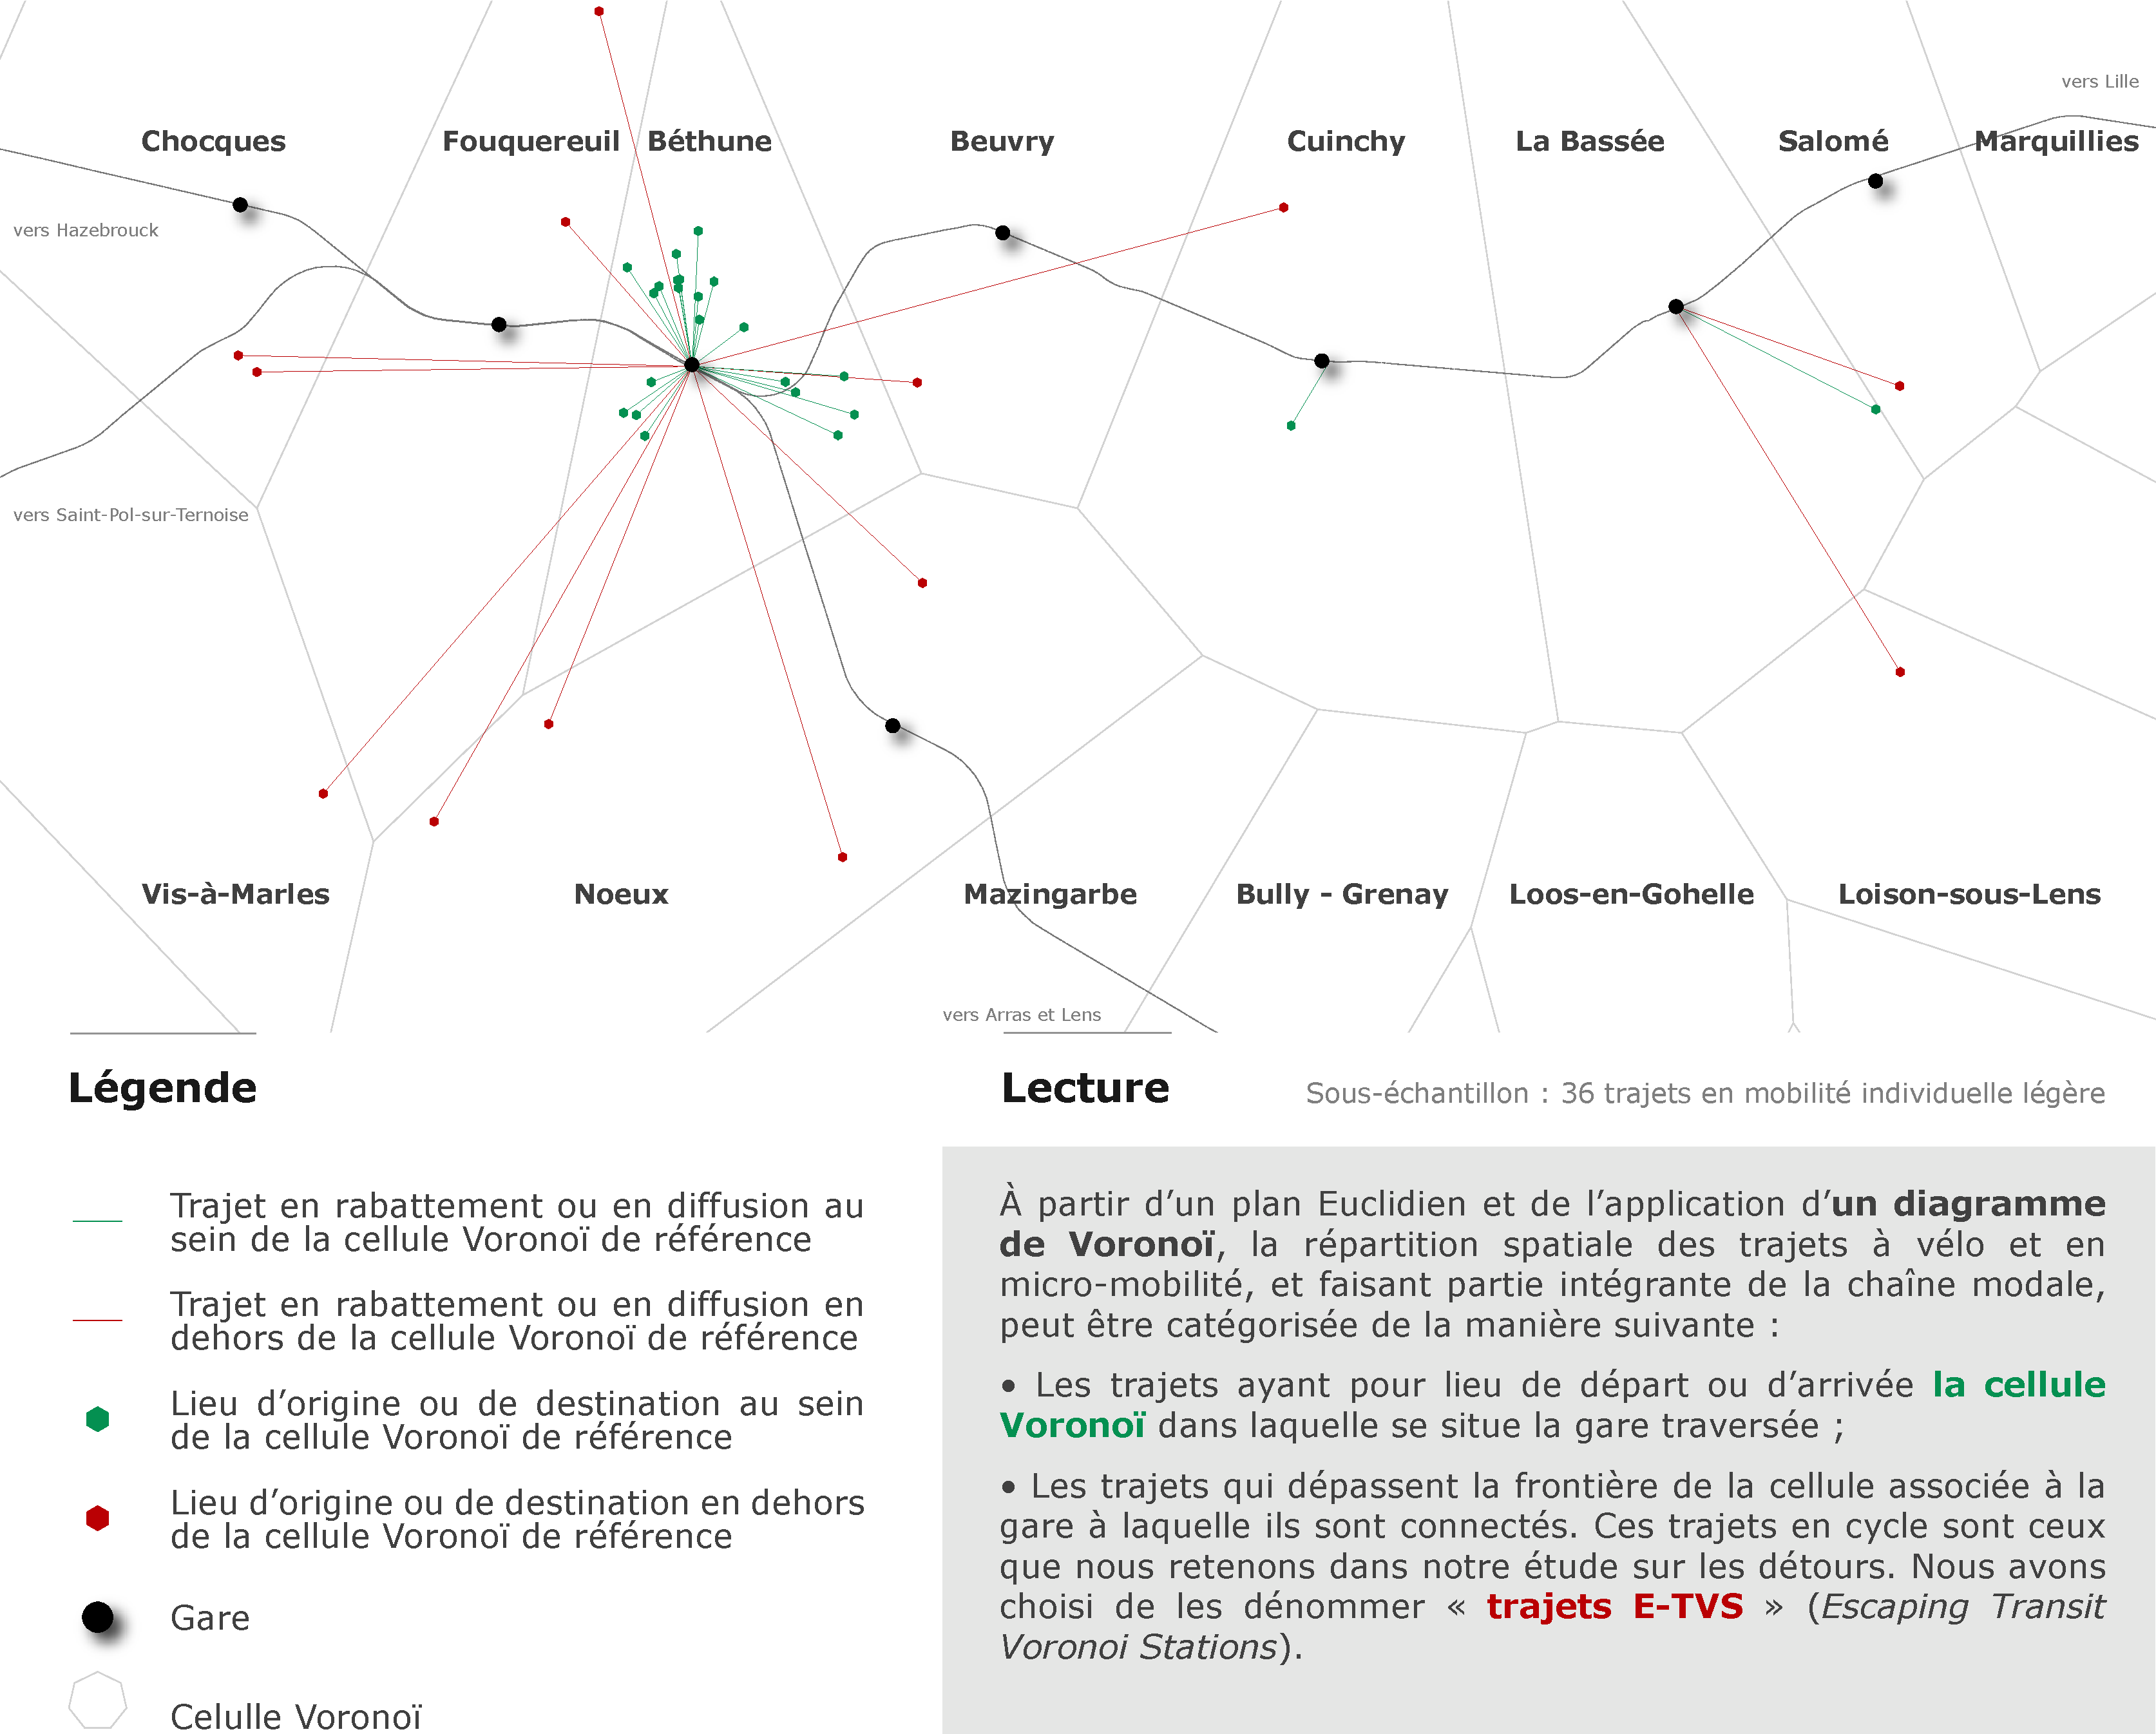
\includegraphics[width=1\columnwidth]{src/Figures/Chap-5/FR_Detours_Diagramme_Voronoi.pdf}}
        \vspace{5pt}
        \begin{flushright}\scriptsize{
        Jeux de données~: \acrshort{GTFS} issues de l'\textsl{Open Data} de la \textcolor{blue}{\textcite{sncf_sncf_2022}}\index{SNCF@\textsl{SNCF}|pagebf} et de la \textcolor{blue}{\textcite{metropole_europeenne_de_lille_opendata_2021}}\index{Métropole Européenne de Lille@\textsl{Métropole Européenne de Lille}|pagebf}
        \\
        Auteur~: \textcolor{blue}{Dylan Moinse (2023)}
        }\end{flushright}
    \end{carte}

    % E-TVS
La production d'une telle technique a donné lieu à la visualisation cartographique apparente sur la \hyperref[fig-chap5:flux-origine-destination-detours]{carte~\ref{fig-chap5:flux-origine-destination-detours}} (page~\pageref{fig-chap5:flux-origine-destination-detours}). Ce type de représentation cartographique prend alors la forme d'un diagramme simplifié de Voronoï axé sur le réseau de transport en commun (\textsl{Simplified Transit Voronoi Diagram}, T-VD), conceptualisé par \textcolor{blue}{\textcite[5]{chen_transit_2022}}\index{Chen, Jieh-Haur|pagebf}\index{Teng, Wenxin|pagebf}\index{Jia, Tao|pagebf}\index{Chen, Hui-Ping|pagebf}\index{Liu, Xianglong|pagebf} et destiné à attribuer la station théoriquement la plus proche à chaque point de départ et de destination.%%Rédigé%%

% Cette analyse cartographique a été améliorée à l'aide de l'utilisation de la transparence des couleurs afin de mettre en relief les matrices de flux symétriques. En effet, l'efficacité de la transparence combinée à un fond noir réside dans l'amélioration de la \Guillemets{saillance visuelle}\footnote{
% La notion de \Guillemets{saillance visuelle}~se réfère à l'adéquation entre le phénomène représenté, les variables visuelles mobilisées et sa perception par l'observateur·rice.
% } des figurés et des informations ainsi que dans la facilitation de la perception des flux de faible valeur tout en garantissant une certaine lisibilité, comme explicité dans la thèse de doctorat de \textcolor{blue}{\textcite[226]{bahoken_contribution_2016}}\index{Bahoken, Françoise|pagebf} sur la cartographie d’une matrice de flux. 

    % 5.3.2.2.
    \needspace{1\baselineskip} % Réserve de l'espace
\subsubsection*{Processus d'échantillonnage
    \label{chap5:echantillonnage-detours-pauses}
    }

    % Echantillonnage
Pour constituer des sous-échantillons axés sur les détours et les pauses (voir l'\hyperref[fig-chap5:echantillonnage-detours-pauses]{illustration~\ref{fig-chap5:echantillonnage-detours-pauses}}, page~\pageref{fig-chap5:echantillonnage-detours-pauses}), le processus d'échantillonnage a capturé les réponses complètes (\textsl{exclusions 1 et 2}), comprenant le dernier déplacement intermodal (\textsl{exclusion 3}), fournissant les coordonnées géographiques valides (\textsl{exclusion 4}), avec un trajet en rabattement et, ou bien, en diffusion réalisé à l'aide du vélo ou d'une option de micro-mobilité et caractérisé par un détour identifié ou une pause déclarée (\textsl{exclusion 5}), et ayant pour motif de déplacement une motivation liée au travail ou aux études (\textsl{exclusion 6}). Il convient de préciser que la définition retenue d'un détour, telle que mobilisée dans cette étude, correspond à l'utilisation d'une station de transport en commun différente de la plus proche du lieu d'origine ou de destination. L'échantillon basé sur les détours comprend 129 déplacements intermodaux, tandis que la taille de l'échantillon basé sur les pauses est de 110 réponses. Soulignons que les déplacements intermodaux comportant un ou des détours et, ou bien, une ou des pauses représentent ainsi respectivement 59~\% et 51~\% des déplacements éligibles. L'identification spatiale des déplacements marqués par la présence de détours a abouti plus spécifiquement à une liste de 171 trajets en rabattement et en diffusion impliquant un détour en mobilité individuelle légère, suggérant que certain·e·s voyageur·se·s réalisent plusieurs détours lors d'un même déplacement. Parmi les voyageur·se·s intermodaux·les ayant effectué un détour (129 déplacements) et signalé une pause (110 déplacements), 73 d'entre elleux ont conjugué les deux pratiques. Plus précisément, 59 d'entre elleux ont opté pour une pause et un détour en vue d'accéder à une station de transport en commun, tandis que 42 l'ont fait pour en sortir. De plus, 28 de ces voyageur·se·s ont combiné une pause et un détour à la fois aux premiers et aux derniers kilomètres de leur déplacement.%%Rédigé%%

   %% Figure échantillonnage détours et pauses
    \begin{figure}[h!]\vspace*{4pt}
        \caption{Processus d'échantillonnage basé sur les détours identifiés et les pauses déclarées dans le cadre du questionnaire administré.}
        \label{fig-chap5:echantillonnage-detours-pauses}
        \centerline{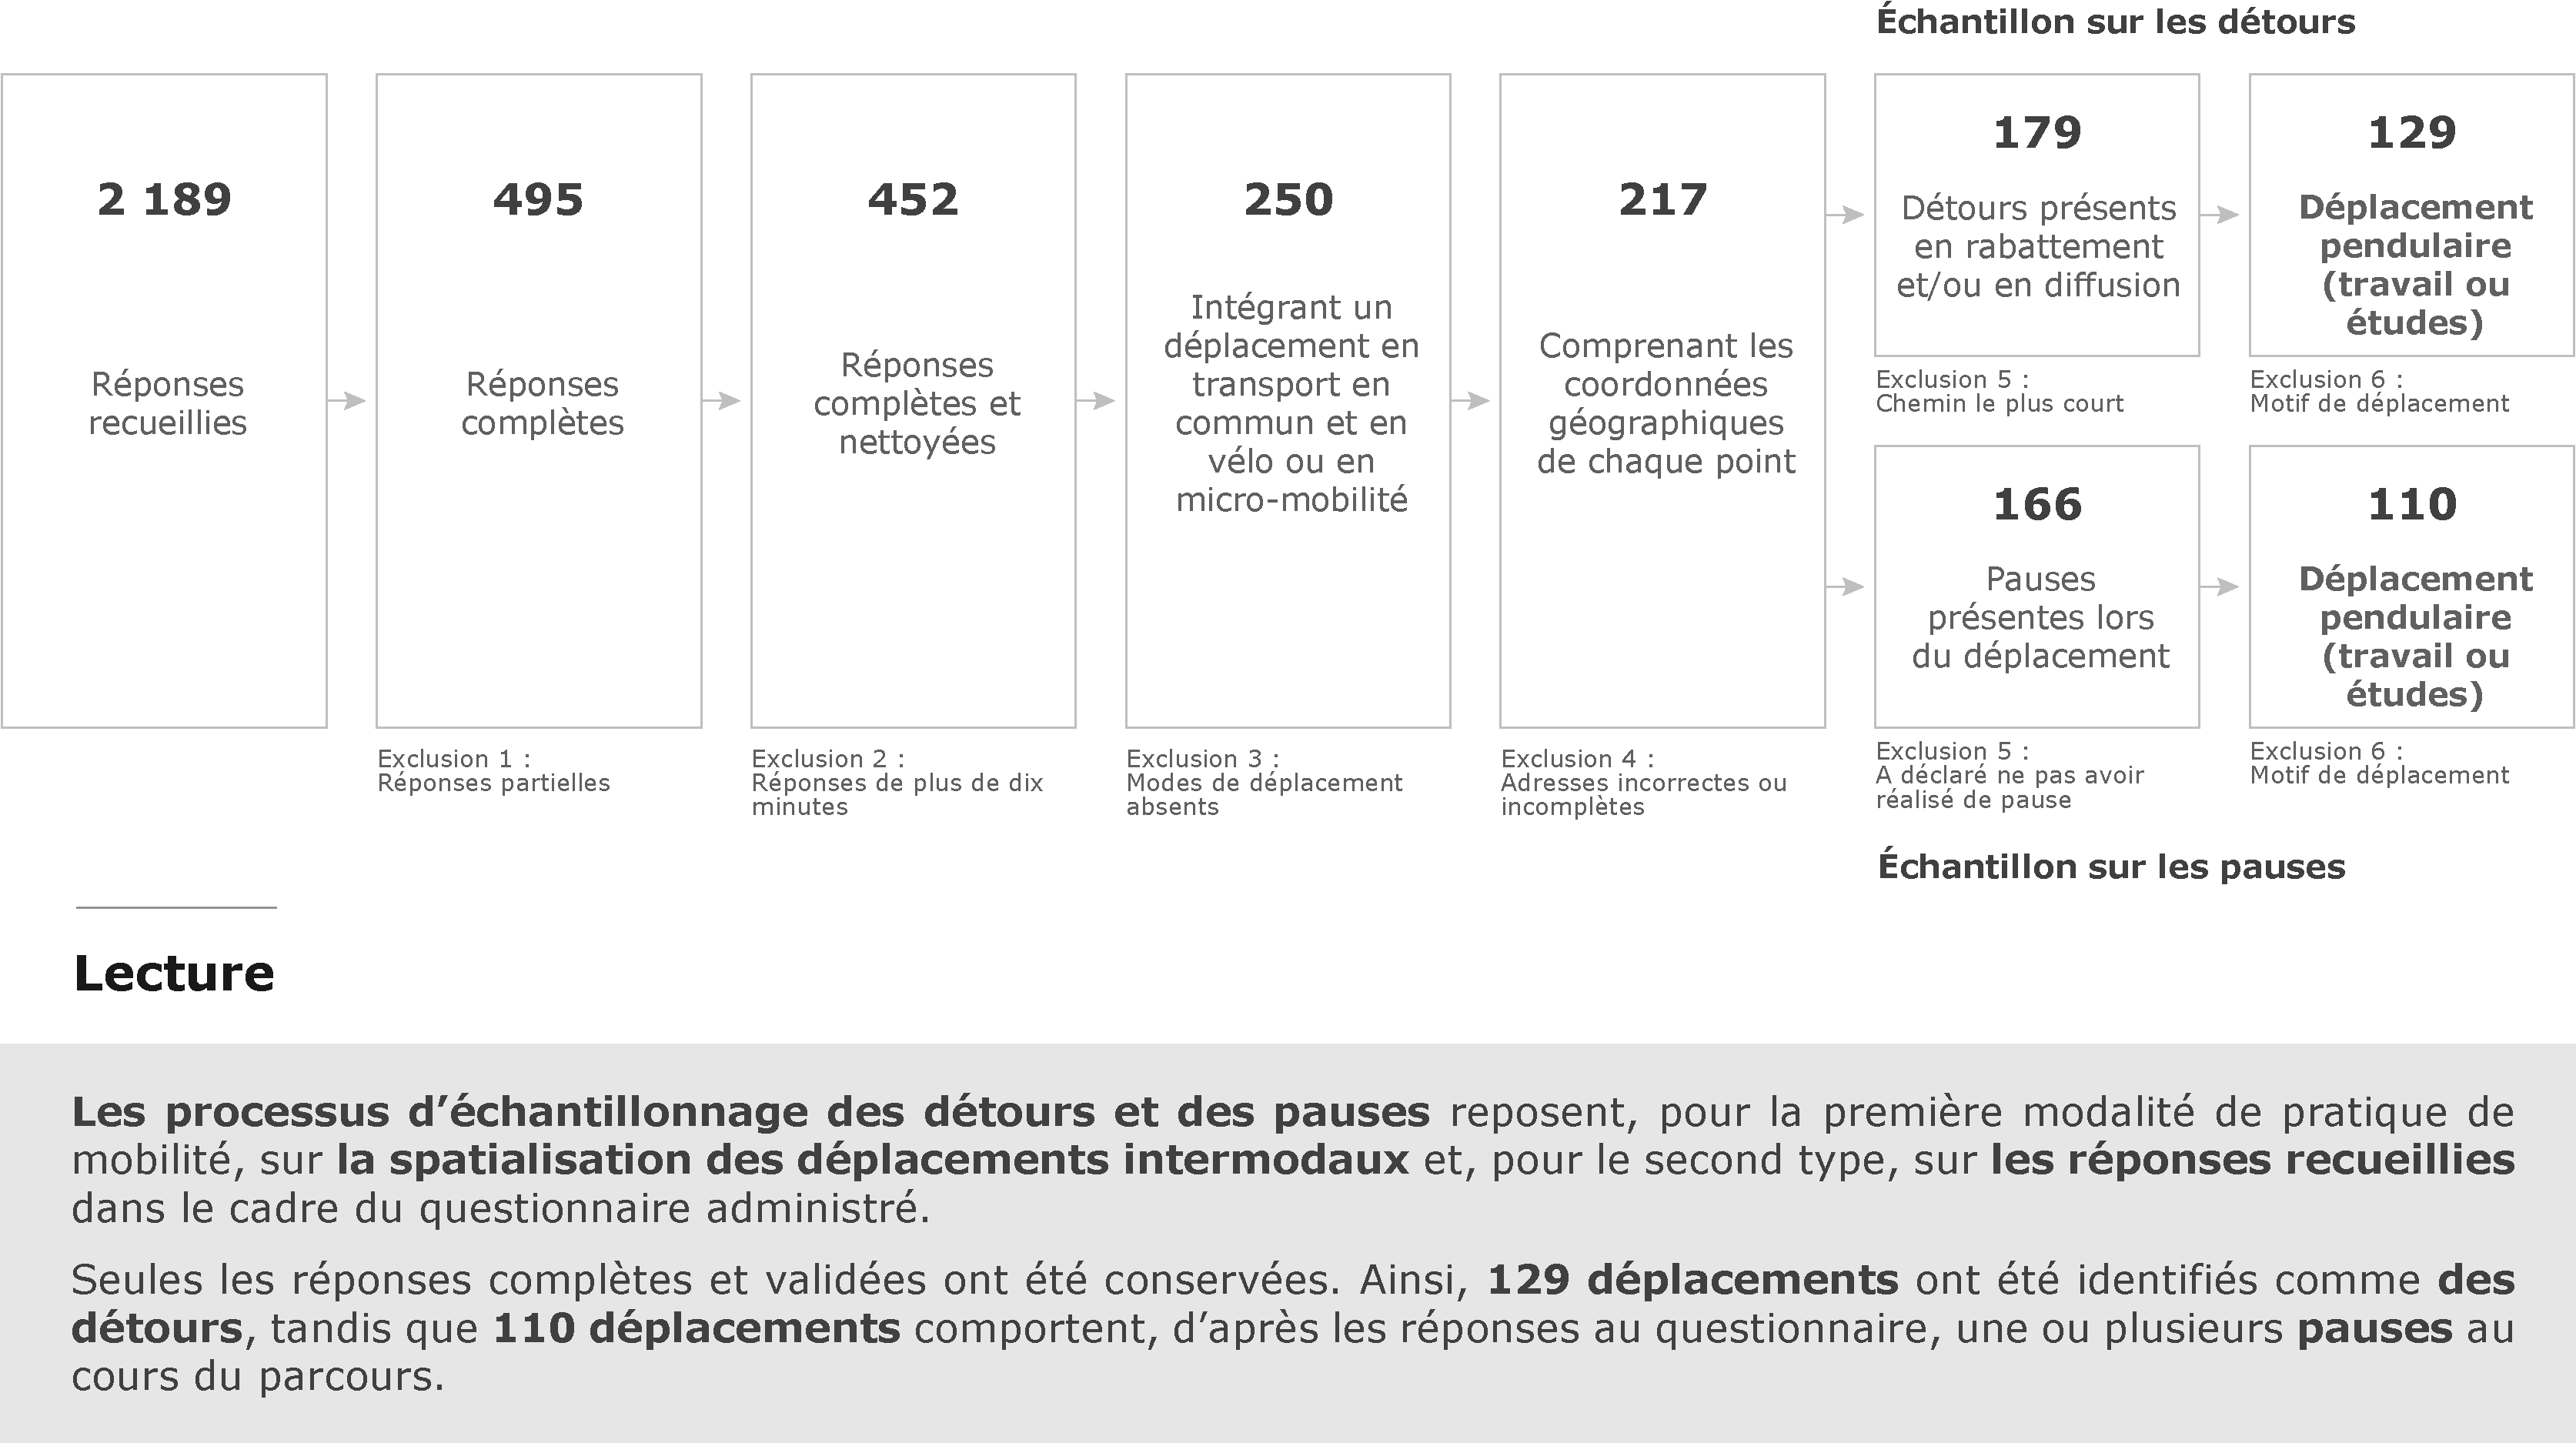
\includegraphics[width=1\columnwidth]{src/Figures/Chap-5/FR_Detours_Echantillonnage.pdf}}
        \vspace{5pt}
        \begin{flushright}\scriptsize{
        Auteur~: \textcolor{blue}{Dylan Moinse (2023)}
        }\end{flushright}
    \end{figure}

    % E-TVS
En entrant les 217 coordonnées géographiques validées associées aux lieux d'origine et de destination reliés aux stations de transport en commun empruntées, 129 déplacements sont ressortis comme ayant une ou plusieurs deux stations ne correspondant pas à la cellule de Voronoï de référence. Parmi les 129 itinéraires identifiés, 83 d'entre eux ont eu lieu dans la région Hauts-de-France. Nous avons nommé ce type de déplacement présentant au moins un détour, intégré dans un contexte d'\gls{intermodalité}, une \Guillemets{station de transport en commun échappant à la cellule de Voronoï}, \acrfull{E-TVS}).%%Rédigé%%

    % Détours et pauses simultanément
Au sein de la population étudiée de voyageur·se·s intermodaux·les ayant à la fois effectué un détour (129 déplacements) et pris une pause (110 déplacements), il ressort que 73 individus ont intégré ces deux activités de manière concomitante. De façon plus détaillée, 59 de ces voyageur·se·s ont réalisé un détour ainsi qu'une pause en pré-acheminement, contre 42 d'entre elleux en post-acheminement, tandis que 28 voyageur·se·s ont réalisé un détour et une pause au cours des deux extrémités du déplacement.%%Rédigé%%

    % 5.3.2.3.
    \needspace{1\baselineskip} % Réserve de l'espace
\subsubsection*{Mesure des ratios d'optimisation spatio-temporelle
    \label{chap5:calcul-ratio-optimisation}
    }

    % Effectif et Alternatif
Deux types différents de déplacement ont été projetés sur \Marque{QGIS}~en important les itinéraires fournis par le planificateur de trajet \Marque{Graphhopper}. Le premier est le déplacement effectif estimé (\(eff\)), qui correspond à l'itinéraire le plus court à partir du réseau et effectivement parcouru par le·la répondant·e et qui intègre un déplacement \acrshort{E-TVS}. Le second représente un scénario de déplacement alternatif hypothétique (\(alt\)) dans lequel l'individu accède à la station de transport en commun la plus proche avec la plus courte distance spatiale. Les itinéraires effectifs sont mesurés en termes de distance spatiale effective\footnote{
    D'après \textcolor{blue}{\textcite[308]{deutsch_note_1961}}\index{Deutsch, Karl~W.|pagebf}\index{Isard, Walter|pagebf}, la \Guillemets{distance effective}~ne peut être simplement mesurée en termes de distance spatiale entre deux points, entités ou individus. Cette notion embrasse une conception multidimensionnelle de la distance concernant un déplacement effectué qui est le produit des distances physiques, économiques (coûts), sociales (quantité et nature des interactions) et relatives à la communication (efficacité et fréquence des échanges). D'autres facteurs peuvent encore influencer la mesure de la distance effective.
} estimée (\(km_{eff}\)) \textcolor{blue}{\autocite[34]{cauvin-reymond_perception_1984}}\index{Cauvin-Reymond, Colette|pagebf}, qui reflète l'équilibre entre les distances objectives \textcolor{blue}{\autocite{brigss_methodologies_1976}}\index{Brigss, Ronald|pagebf} et cognitives, subjectives et perçues \textcolor{blue}{\autocite{canter_psychology_1977, bailly_perception_1977, sadalla_perception_1980}}\index{Canter, David~V.|pagebf}\index{Bailly, Antoine|pagebf}\index{Sadalla, Edward~K.|pagebf}\index{Magel, Stephen~G.|pagebf}, et par les valeurs de distance-temps effective (\(t_{eff}\)), qu'elles soient objectives (\(t_{eff_{(O)}}\)) ou perçues (\(t_{eff_{(P)}}\)). De même, le déplacement alternatif est décrit par des paramètres de distance spatiale (\(km_{alt}\)) et de distance-temps alternatives (\(t_{alt_{(O)}}\) et \(t_{alt_{(P)}}\)), comme le montrent les \hyperref[equation-chap5:effectif-alternatif]{formules~\ref{equation-chap5:effectif-alternatif}} (page~\pageref{equation-chap5:effectif-alternatif}) suivantes~:%%Rédigé%%

    \begin{equation}
    \label{equation-chap5:effectif-alternatif}
    \begin{array}{lclclclclclcl}
    \displaystyle km_{alt} = km_{R(alt)} + km_{TC(alt)} + km_{D(alt)}\\\\
    \displaystyle km_{eff} = km_{R(eff)} + km_{TC(eff)} + km_{D(eff)}\\\\
    \displaystyle t_{alt_O} = t_{R(alt_O)} + t_{TC(alt_O)} + t_{D(alt_O)}\\\\
    \displaystyle t_{eff_O} = t_{R(eff_O)} + t_{TC(eff_O)} + t_{D(eff_O)}\\\\
    \displaystyle t_{alt_P} = 1.8*t_{R(alt_P)} + 2.8*t_{A(alt_P)} + 1*t_{TC(alt_P)} + 1.8*t_{D(alt_P)}\\\\
    \displaystyle t_{eff_P} = 1.8*t_{R(eff_P)} + 2.8*t_{A(eff_P)} + 1*t_{TC(eff_P)} + 1.8*t_{D(eff_P)}
    \end{array}
    \end{equation}

\begin{align*}
    &\text{où~:} \\
    _R &\text{ représente le trajet en rabattement vers la station~;} \\
    _D &\text{ représente le trajet en diffusion depuis la station~;} \\
    _{TC} &\text{ représente le(s) trajet(s) en transport en commun~;} \\
    _A &\text{ représente le temps d'attente lors d'une correspondance.}
\end{align*}

    % Explication équation
Sachant que \(t_{eff_{(P)}}\) et \(t_{alt_{(P)}}\) sont mesurés à l'aide de pondérations spécifiques à chacune des composantes du déplacement, à savoir les trajets en rabattement et en diffusion, ainsi que le temps d'attente, ayant respectivement une valeur de temps perçue 1,8 fois supérieure \textcolor{blue}{\autocite[110]{wardman_review_2001, gleave_transport_1997}}\index{Wardman, Mark|pagebf}\index{Gleave, Steer Davies|pagebf} et 2,8 fois supérieure \textcolor{blue}{\autocite[110]{horl_introducing_2021, wardman_review_2001}}\index{Hörl, Sebastian|pagebf}\index{Balac, Milos|pagebf}\index{Wardman, Mark|pagebf} par rapport au temps à bord du mode collectif principal. Cette multiplication du temps intègre de manière plus réaliste le temps d'attente et de déplacement à vélo ou en micro-mobilité dans la formule du temps perçu. Le temps d'attente nécessaire pour un mode de transport en commun est estimé en fonction des heures de pointe pour ces déplacements domicile-travail ou domicile-études et varie en fonction du type de transport en commun utilisé. Un temps de précaution d'une valeur de quinze minutes est supposé pour le \acrshort{TGV} et l'Intercité \textcolor{blue}{\autocite[12]{pagliara_high-speed_2012}}\index{Pagliara, Francesca|pagebf}\index{Vassallo, José Manuel|pagebf}\index{Román, Concepción|pagebf}, de dix minutes pour le \acrshort{TER} et le Transilien \textcolor{blue}{\autocite[300]{ingvardson_passenger_2018}}\index{Ingvardson, Jesper Bláfoss|pagebf}\index{Nielsen, Otto Anker|pagebf}\index{Raveau, Sebastián|pagebf}\index{Nielsen, Bo Friis|pagebf}, et de cinq minutes pour le \acrshort{RER}, le métro et le tramway \textcolor{blue}{\autocite[300]{hua_comprehensive_2018, ingvardson_passenger_2018}}\index{Hua, Weixin|pagebf}\index{Feng, Xuesong|pagebf}\index{Zhu, Xiaojing|pagebf}\index{Jie, Yuanpeng|pagebf}\index{Ingvardson, Jesper Bláfoss|pagebf}\index{Nielsen, Otto Anker|pagebf}\index{Raveau, Sebastián|pagebf}\index{Nielsen, Bo Friis|pagebf}.%%Rédigé%%

    % Ratios
Le niveau de détour a été mesuré à partir du rapport entre l'itinéraire effectif (\(eff\)) et sa distance spatiale par rapport à un itinéraire sans détour (\(alt\)) et à la distance euclidienne (\(eud\)). Ces deux rapports sont employés dans la littérature scientifique, le premier sous le nom d'\acrfull{RDI}, ou indice de Directivité de l'Itinéraire, dont l'intérêt est de mesurer la connectivité par rapport à une distance euclidienne \textcolor{blue}{\autocite[193]{park_why_2019}}\index{Park, Yujin|pagebf}\index{Akar, Gulsah|pagebf}, et le second sous le nom d'\acrfull{GRDI}, ou indice de directivité géographique de l'itinéraire, par rapport au chemin le plus court sur un réseau \textcolor{blue}{\autocite[126]{ciscal-terry_analysis_2016}}\index{Ciscal-Terry, Wilner|pagebf}\index{Dell'Amico, Mauro|pagebf}\index{Hadjidimitriou, Natalia Selini|pagebf}\index{Iori, Manuel|pagebf}. Dans le contexte de ce travail de recherche cherchant à revisiter le détour comme un moyen d'optimiser de manière spatio-temporelle les déplacements, l'indicateur initialement prévu pour calculer le taux de circuité (\acrshort{GRDI}) a été inversé pour capturer les différences résultant des détours. Nous avons ainsi appelé le \acrshort{GRDI} adapté à notre étude le \Guillemets{Ratio d'optimisation}, noté \(R\). Le taux d'optimisation est défini en distance spatiale (\(R_{km}\)) et en distance-temps, déclinée en temps objectif (\(R_{t{(O)}}\)) et perçu (\(R_{t_{(P)}}\)), tels qu'exprimés dans les \hyperref[equation-chap5:ratios-optimisation]{formules~\ref{equation-chap5:ratios-optimisation}} (page~\pageref{equation-chap5:ratios-optimisation}).%%Rédigé%%

    \begin{equation}
    \label{equation-chap5:ratios-optimisation}
    \begin{array}{lclcl}
    \displaystyle R_{km} = \displaystyle\frac{km_{alt}}{km_{eff}}\\\\
    \displaystyle R_{t_O} = \displaystyle\frac{t_{alt_O}}{t_{eff_O}}\\\\
    \displaystyle R_{t_P} = \displaystyle\frac{t_{alt_P}}{t_{eff_P}}\\\\
    \end{array}
    \end{equation}

    % 5.3.2.4.
    \needspace{1\baselineskip} % Réserve de l'espace
\subsubsection*{Calcul des angles des déplacements \acrshort{E-TVS}
    \label{chap5:calcul-angles-detours}
    }

    % Inversion spatiale
Afin de répondre à une autre sous-hypothèse de recherche formulée précédemment, cette étude s'intéresse à la mesure des angles des trajets à vélo ou en micro-mobilité, de manière à conduire une analyse statistique et géométrique de ces flux. L'angle qui définit un trajet du lieu d'origine à la gare d'arrivée, en passant par la gare de départ, ou encore de la gare de départ jusqu'au lieu de destination en passant par la gare d'arrivée, permet de mieux comprendre si ces déplacements \acrshort{E-TVS} présentent des différences géométriques par rapport aux déplacements alternatifs. La détermination des angles est alors un moyen de comprendre si le choix des détours s'accompagne d'une intégration du facteur lié aux angles. Dans le contexte de la mobilité, il est considéré qu'un angle, dit extrême et présentant un détour géométrique important, est qualifié d'\Guillemets{inversion spatiale}. L'inversion spatiale se réfère à la démarche consistant à emprunter une voie en sens inverse de celle menant au point de destination, dans le but d'accéder à certains réseaux de transport. Dans le cadre de cette section consacrée aux détours intermodaux réalisés à l'aide de la mobilité individuelle légère, les usager·ère·s ont l'opportunité d'effectuer une inversion spatiale à partir de leur point de départ (\(A\)) en se dirigeant dans la direction opposée afin d'atteindre la station de départ (\(B\)), plutôt que dans le sens de leur destination (\(C\)). Ce choix s'opère généralement dans l'objectif d'accéder à un système de transport efficient, tel que les réseaux de transport en commun.%%Rédigé%%

    % Calcul angles
Pour calculer l'angle $\widehat{ABC}$, noté $\alpha$, en utilisant les coordonnées géographiques recueillies, nous mobilisons des concepts de la trigonométrie sphérique et de la géométrie dans le plan euclidien. La trigonométrie sphérique est une branche de la trigonométrie qui s'applique aux objets situés sur une sphère, tels que la Terre\footnote{
Il convient de noter que ce calcul suppose que les points \(A\), \(B\) et \(C\) se trouvent sur une sphère idéalisée, semblable à la Terre, et que les coordonnées géographiques sont précises. En réalité, des approximations et des corrections supplémentaires peuvent s'avérer nécessaires en fonction de la projection cartographique utilisée et des caractéristiques de la surface terrestre. 
}. Par les formules de la trigonométrie sphériques, nous convertissons les coordonnées géographiques dans un repère cartésien, puis nous nous plaçons dans un plan euclidien en négligeant la courbure terrestre. Les étapes permettant de déterminer l'angle $\alpha$ sont les suivantes~: (i) la détermination des coordonnées géographiques des points \(A\), \(B\) et \(C\)~; (ii) la conversion des coordonnées géographiques en coordonnées cartésiennes (\(x\), \(y\), \(z\))~; (iii) le calcul des normes $\lVert \vec{AB} \rVert$ et $\lVert \vec{BC} \rVert$ des vecteurs $\vec{AB}$ et $\vec{BC}$~; (iv) le calcul du produit scalaire de $\vec{AB}$ et $\vec{BC}$~; et (v) la mesure de l'angle en radians ainsi que sa conversion en degrés ($\alpha$) (voir l'\hyperref[fig-chap5:inversion-spatiale-detours]{illustration~\ref{fig-chap5:inversion-spatiale-detours}}, page~\pageref{fig-chap5:inversion-spatiale-detours}).%%Rédigé%%

   %% Figure calcul angles E-TVS
    \begin{figure}[h!]\vspace*{4pt}
        \caption{Schéma des angles des déplacements impliquant un détour géométrique en lien avec la notion d'inversion spatiale.}
        \label{fig-chap5:inversion-spatiale-detours}
        \centerline{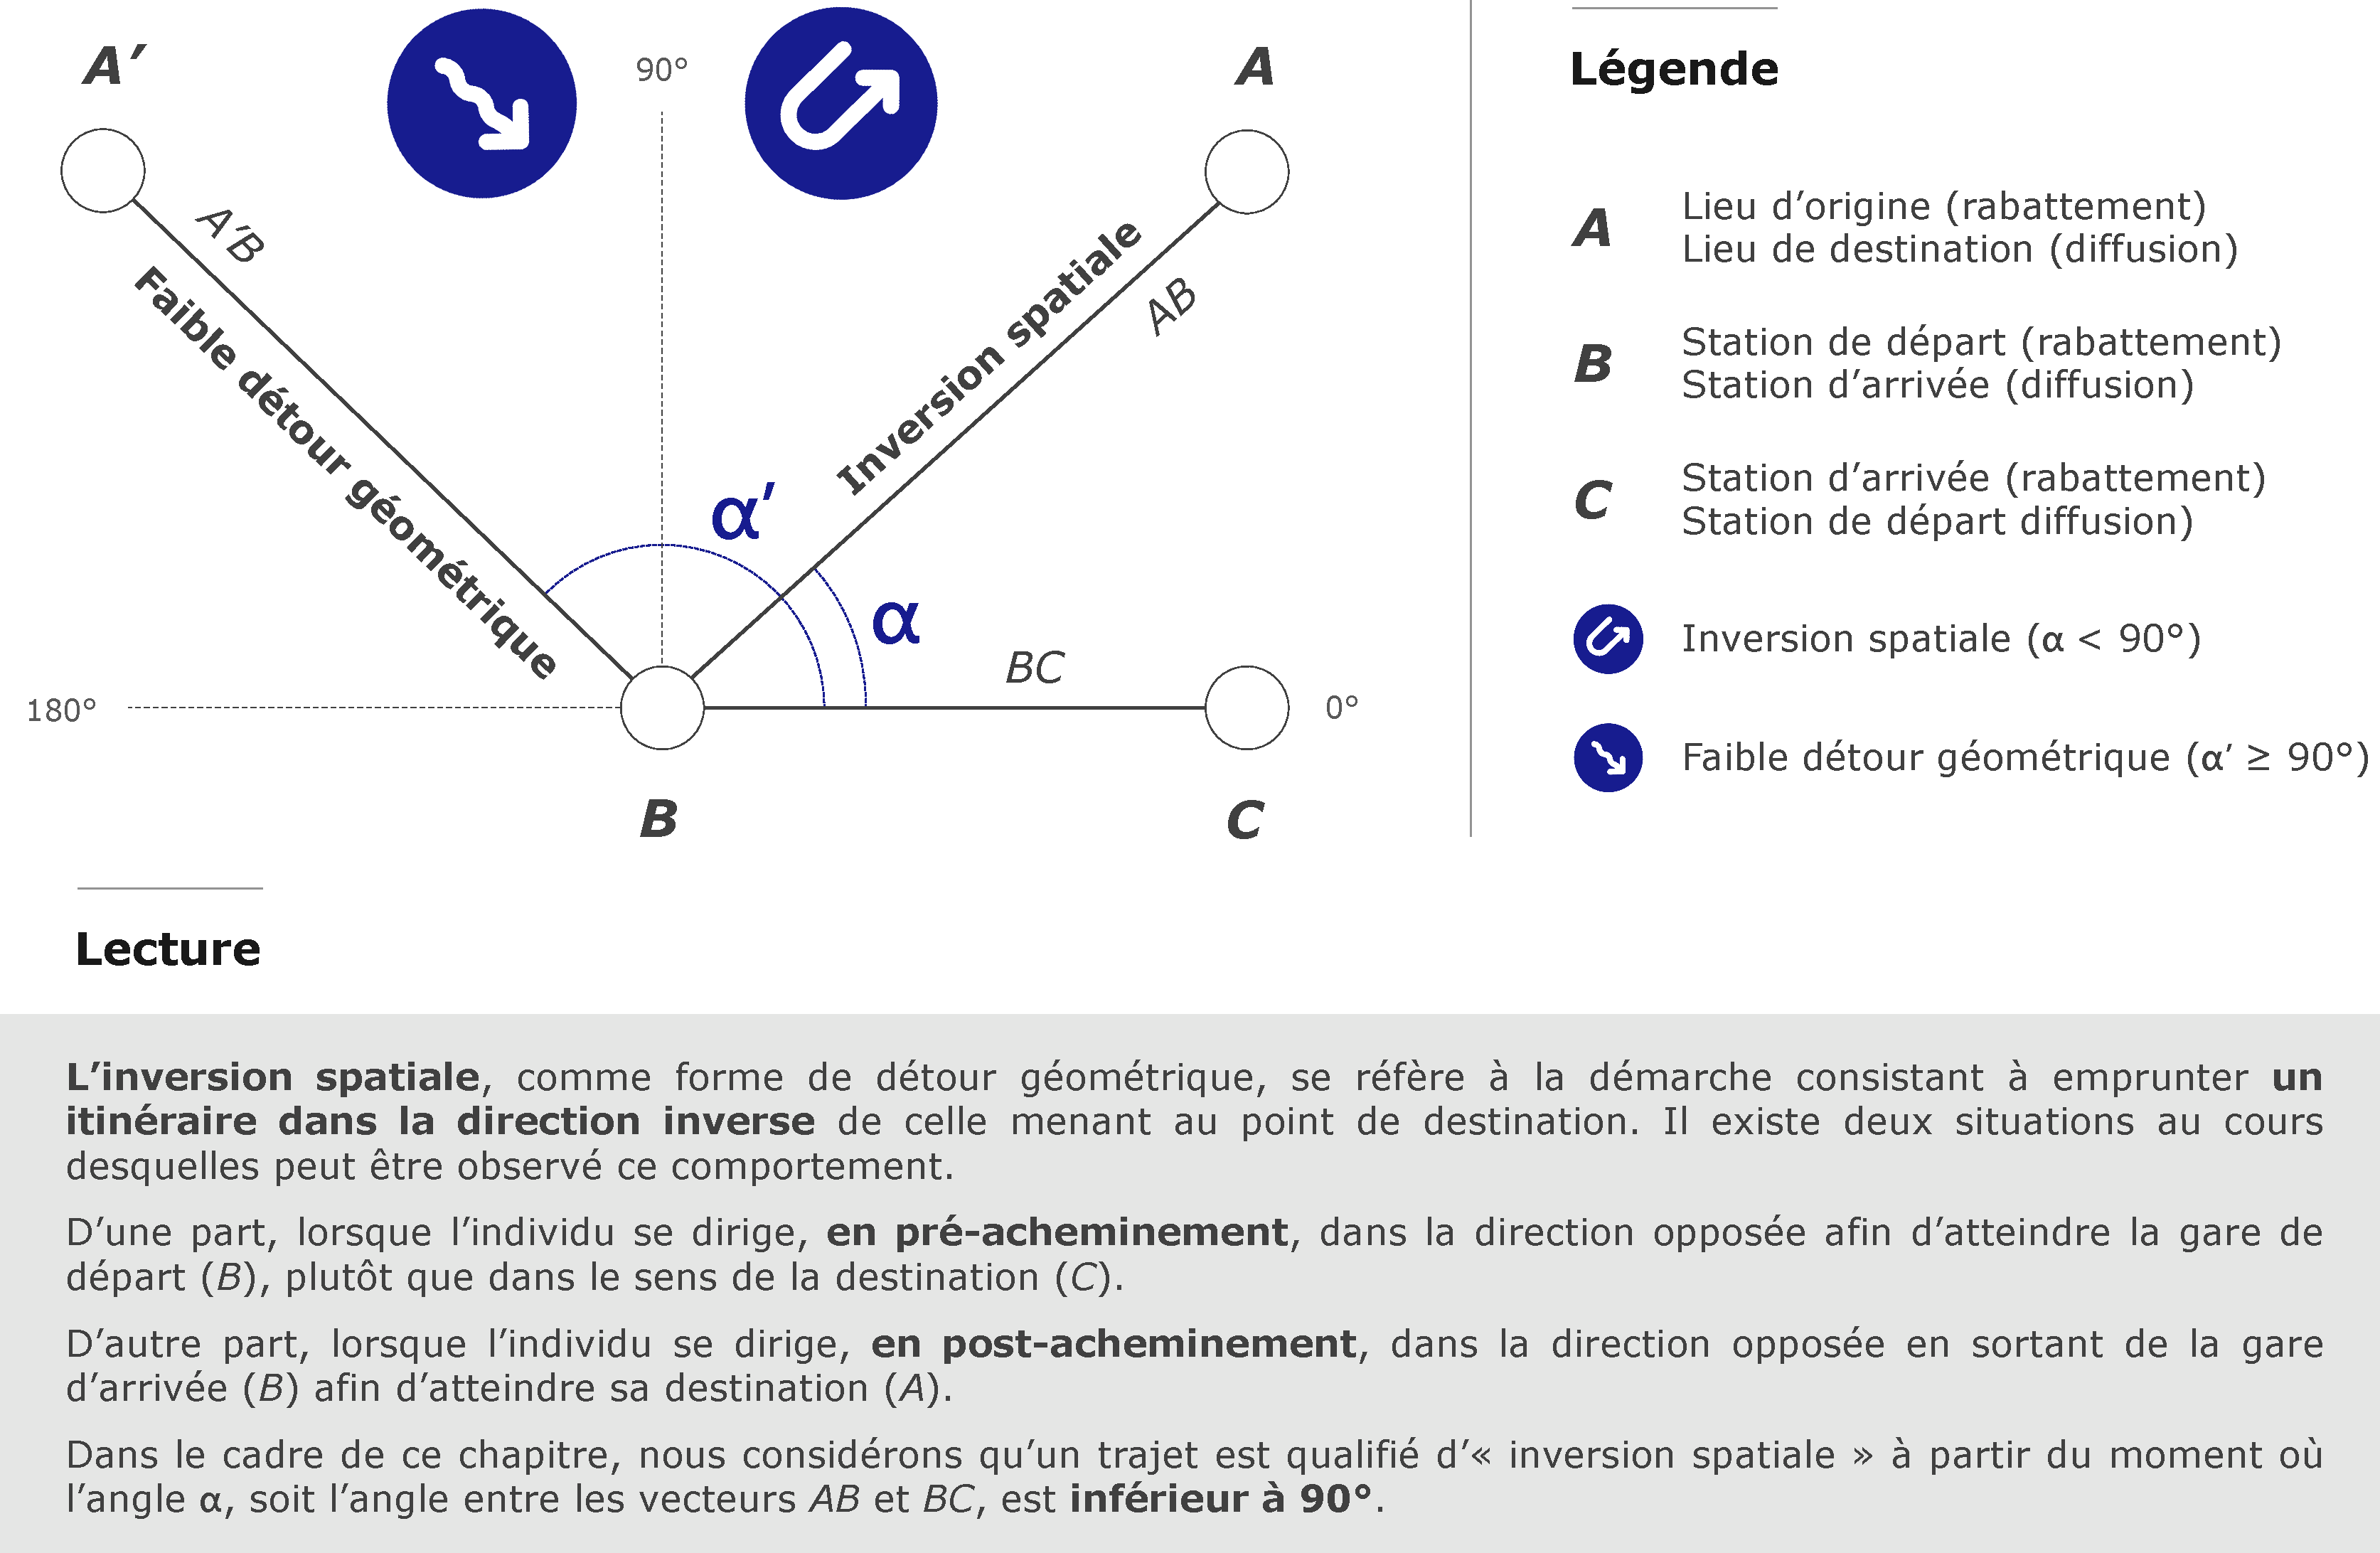
\includegraphics[width=1\columnwidth]{src/Figures/Chap-5/FR_Detours_Calcul_angles.pdf}}
        \vspace{5pt}
        \begin{flushright}\scriptsize{
        Auteur~: \textcolor{blue}{Dylan Moinse (2023)}
        }\end{flushright}
    \end{figure}

    % Coordonnées cartésiennes
Après avoir obtenu les coordonnées géographiques des points \(A\), \(B\) et \(C\), exprimées en latitude et en longitude en utilisant le système de projection \acrshort{WGS84}\footnote{
La projection \acrfull{WGS84} est un système de coordonnées géographiques utilisé pour définir la forme et la position de la Terre. Il est notamment employé comme base pour les systèmes de positionnement par satellite tels que le \acrfull{GPS}.
}, nous les avons converties en coordonnées cartésiennes (\(x\), \(y\), \(z\)) en recourant aux formules de conversion applicables à une sphère. Par la suite, en soustrayant les coordonnées cartésiennes des points \(A\) et \(B\), puis \(B\) et \(C\), nous avons calculé les normes $\lVert \vec{AB} \rVert$ et $\lVert \vec{BC} \rVert$. Ces vecteurs ont été par la suite exploités pour déterminer leur produit scalaire respectif ($\vec{AB} \cdot \vec{BC}$). En définitive, nous avons été à même de déduire l'angle entre les vecteurs $\vec{AB}$ et $\vec{BC}$, exprimé en radians puis en degrés ($\alpha$). Les calculs détaillés des angles ont notamment été renseignés dans l'\hyperref[annexes:calcul-detours-angles]{annexe~\ref{annexes:calcul-detours-angles}} (page~\pageref{annexes:calcul-detours-angles}).%%Rédigé%%

    % Explications
Une fois les angles $\alpha$ mesurés, nous avons généré une grille d'analyse en vue de catégoriser les angles des déplacements \acrshort{E-TVS} déterminés. En identifiant les formes d'écartement extrême comme une inversion spatiale, survenant lorsque l'angle $\alpha$ est compris entre 0° à 90°, nous sommes en mesure de distinguer les déplacements qui comprennent des détours géométriques conséquents et des trajets rectilignes.%%Rédigé%%

    % 5.3.3.
    \needspace{1\baselineskip} % Réserve de l'espace
\subsection{Caractérisation des stratégies d'optimisation
    \label{chap5:strategies-optimisation}
    }

    % Introduction
Cette section présente les résultats issus de l'analyse statistique des déplacements intégrant des détours et des pauses. Le premier résultat décrit portera sur les distances mesurées des déplacements \acrshort{E-TVS}, en identifiant plus particulièrement les distances parcourues pour effectuer un détour. La détermination des distances-temps et spatiales relatives aux détours permettra, dans un second temps, d'évaluer les ratios d'optimisation spatio-temporelle des déplacements \acrshort{E-TVS}. Une fois que l'étude aura démontré les liens positifs existant entre la présence de détours et la recherche d'optimisation du mouvement, l'étude s'attachera à classer les différents types de stratégies d'optimisation par le biais de détours et de pauses. Enfin, le dernier résultat exposera la catégorisation des usager·ère·s effectuant des détours en intermodalité, en fonction des ratios d'optimisation déterminés.%%Rédigé%%

    % 5.3.3.1.
    \needspace{1\baselineskip} % Réserve de l'espace
\subsubsection*{Une extension accrue de la zone de pertinence de la mobilité individuelle légère autour des gares
    \label{chap5:extension-accrue-quartier-gare}
    }

    % Analyse
Avant d'envisager les détours, il est impératif de déterminer les distances parcourues par les utilisateur·rice·s du vélo et de la micro-mobilité, aussi bien pour les trajets en rabattement qu'en diffusion, afin d'évaluer les dimensions des aires d'influence autour des stations de transport en commun. Les distances-temps et spatiales ont pu être calculées à partir des coordonnées géographiques recueillies dans le cadre du questionnaire diffusé dans cette recherche doctorale. Pour mesurer la distance socialement acceptable des détours réalisés par les répondant·e·s, la valeur du 85\textsuperscript{e} centile a été également retenue dans la distribution cumulative appliquée \textcolor{blue}{\autocite[982]{lee_bicycle-based_2016}}\index{Lee, Jaeyeong|pagebf}\index{Choi, Keechoo|pagebf}\index{Leem, Yountaik|pagebf}.%%Rédigé%%

    % Distances
En portant une attention particulière au sous-échantillon composé de 129 déplacements \acrshort{E-TVS}, et plus précisément aux 171 trajets à vélo ou en micro-mobilité, et en rabattement ou en diffusion, caractérisés par la présence de détours, l'estimation des distances pour de tels trajets sont, sans surprise, plus élevées. Tous types de mobilité individuelle légère confondus, ces trajets \acrshort{E-TVS} comportent une distance spatiale acceptable de 6,1 kilomètres en pré-acheminement et de 5,2 kilomètres en post-acheminement, pour une médiane respective de 2,7 et de 2,3 kilomètres. Parmi les divers véhicules examinés figure en premier lieu le vélo classique (78 trajets), atteignant une longueur de 6,7 kilomètres et une médiane de 2,5 kilomètres, suivi du vélopartage et de la micro-mobilité partagée (17 trajets) avec 4,4 et 2,9 kilomètres, du vélo pliant (18 trajets) avec 6,5 et 2,4 kilomètres et de la \acrshort{TEP} (36 trajets) avec 5,7 et 2,5 kilomètres.%%Rédigé%%

    % Distances détours
En comparaison avec la distance spatiale estimée des trajets alternatifs (\(alt\)) réalisés à vélo ou en micro-mobilité, les trajets \acrshort{E-TVS} (\(eff\)), notamment en pré-acheminement, couvrent des distances spatiales plus importantes. En confrontant les trajets avec et sans détour, l'analyse statistique révèle une distance spatiale supplémentaire conséquente pour ces derniers, d'environ deux kilomètres, soit une distance-temps additionnelle de dix minutes. Ainsi, les utilisateur·rice·s génèrent en moyenne des détours équivalents à deux kilomètres, représentant près d'un tiers de la distance totale parcourue en rabattement et en diffusion par les voyageur·se·s intermodaux·les ayant recours à la mobilité individuelle légère. Cette mesure liée à la distance spatiale additionnelle portée par les voyageur·se·s entre alors en résonance avec la recherche empirique de \textcolor{blue}{\textcite[11]{jin_competition_2019}}\index{Jin, Haitao|pagebf}\index{Jin, Fengjun|pagebf}\index{Wang, Jiao'e|pagebf}\index{Sun, Wei|pagebf}\index{Dong, Libo|pagebf} démontrant que les usager·ère·s en métro et en bus tendent à remplacer les courtes correspondances en transport en commun urbain, de moins de deux kilomètres, par l'usage du \acrshort{VFF} à Beijing.%%Rédigé%%

    % 5.3.3.2.
    \needspace{1\baselineskip} % Réserve de l'espace
\subsubsection*{Les détours, catalyseurs d'économie de distance
    \label{chap5:detours-gains-de-temps}
    }

    % Taux de détour
En croisant les distances spatiales observées (\(km_{eff}\)) avec les distances spatiales issues des déplacements alternatifs désignées (\(km_{alt}\)), nous sommes alors en mesure de déterminer le taux de détour des 129 déplacements pendulaires \acrshort{E-TVS}. Le taux de détour, tel qu'explicité dans la méthode d'analyse statistique, est un indicateur dont une valeur supérieure à 1 indique que l'itinéraire effectif est plus long que l'itinéraire le plus court. Il apparaît que le taux de détour moyen est de 0,97 pour l'ensemble des déplacements, avec une médiane de 0,98 (voir le \hyperref[table-chap5:taux-detours]{tableau~\ref{table-chap5:taux-detours}}, page~\pageref{table-chap5:taux-detours}). Du point de vue statistique, ce ratio présente un écart-type de 0,07, avec une valeur minimale de 0,7 et une valeur maximale de 1,21. De manière générale, les déplacements \acrshort{E-TVS} effectués à vélo ou en micro-mobilité semblent présenter paradoxalement des distances spatiales relativement plus courtes que les trajets alternatifs sans détours. En outre, le ratio moyen entre les distances spatiales effectives et alternatives est de 5,75 pour les itinéraires en pré-acheminement (89 trajets) et de 7,73 pour les itinéraires en post-acheminement (81 trajets). Ces écarts substantiels laissent à penser que les cyclistes intermodaux·les préfèrent délibérément effectuer des détours six à huit fois plus longs en moyenne afin de réaliser des économies de distance spatiale sur l'ensemble de leur déplacement intermodal.%%Rédigé%%

    % Tableau Statistiques descriptives taux de détour E-TVS
% Tableau Statistiques descriptives taux de détour E-TVS
%%Rédigé%%
    \begin{table}[h!]
    \centering
    \renewcommand{\arraystretch}{1.5}
    \resizebox{\columnwidth}{!}{
    \begin{tabular}{p{0.47\columnwidth}p{0.1\columnwidth}p{0.1\columnwidth}p{0.11\columnwidth}p{0.11\columnwidth}p{0.11\columnwidth}}
        %\hline
    \rule{0pt}{15pt} \textcolor{blue}{\textbf{Itinéraires}} & \textcolor{blue}{\textbf{Taux}} & \textcolor{blue}{\textbf{$\sigma$}} & \textcolor{blue}{\textbf{Min.}} & \textcolor{blue}{\textbf{Max.}} & \textcolor{blue}{\textbf{Effectif}}\\
        \hline
    \multicolumn{6}{l}{\textbf{Déplacement global}}\\
\small{Déplacement intermodal~($ km_{eff} $/$ km_{alt} $)} & \small{0,97} & \small{0,07} & \small{0,70} & \small{1,21} & \small{129}\\
        \hdashline
    \multicolumn{4}{l}{\textbf{Segments du déplacement}}\\
\small{Trajet en rabattement~($ km^{R}_{eff} $/$ km^{R}_{alt} $)} & \small{5,75} & \small{7,30} & \small{1,05} & \small{46,73} & \small{89}\\
\small{Trajet en diffusion~($ km^{D}_{eff} $/$ km^{D}_{alt} $)} & \small{7,73} & \small{14,23} & \small{1,09} & \small{115,22} & \small{81}\\
\small{Trajet en TC~($ km^{TC}_{eff} $/$ km^{TC}_{alt} $)} & \small{0,90} & \small{0,12} & \small{0,45} & \small{1,15} & \small{129}\\
        \hline
        \end{tabular}}
    \caption{Taux de détour des déplacements pendulaires, impliquant un détour.}
    \label{table-chap5:taux-detours}
        \vspace{5pt}
        \begin{flushleft}\scriptsize{
        \textcolor{blue}{Note~:} $\sigma$~correspond à l'écart-type.
        \\
        \textcolor{blue}{Lecture~:} les taux de détour des déplacements pendulaires montrent que les segments de rabattement et de diffusion affichent des détours très élevés, mais que ceux-ci sont compensés par un déplacement global proche de l'itinéraire optimal.
        }\end{flushleft}
        \begin{flushright}\scriptsize{
        Auteur~: \textcolor{blue}{Dylan Moinse (2023)}
        }\end{flushright}
        \end{table}%%Rédigé%%

    % Taux de circuité
La détermination contre-intuitive du taux de détour est étayée par la mesure du coefficient de circuité qui prend en compte la distance spatiale effective du déplacement \acrshort{E-TVS} (\(km_{eff}\)) et la distance spatiale du flux à vol d'oiseau sans détour (\(km_{eud}\)). À cet égard, le taux de circuité global du déplacement \acrshort{E-TVS} révèle une distance spatiale supplémentaire de 53~\%, avec un taux de circuité en pré-acheminement (89 trajets) 8,34 fois plus élevé et un taux de circuité en post-acheminement (81 trajets) 29,91 fois plus élevé. Par ailleurs, l'analyse statistique du taux de circuité, basé sur la distance euclidienne, ainsi que du taux de détour, fondé sur la station de transport en commun la plus proche, met en évidence une asymétrie entre les premiers et les derniers kilomètres. En effet, le trajet se déployant à la sortie de la station est marqué par des détours nettement plus prononcés que ceux observés en la rejoignant. Plus précisément, le coefficient de circuité en diffusion est 3,59 fois plus important tandis que le coefficient de détour en diffusion est quant à lui 1,34 fois supérieur.%%Rédigé%%

    % Détours temps
La relation positive entre les détours et les économies de distance peut également se traduire par une analyse examinant la distance-temps des déplacements \acrshort{E-TVS}. Alors que le temps objectif total moyen (\(t_{O}\)) économisé est de 18,82~\% et que le temps perçu (\(t_{P}\)) est de 17,56~\%, ce qui illustre le processus d'optimisation en jeu, \(t_{access}\) et \(t_{egress}\) sont respectivement 3,12 et 3,59 fois plus longs que les trajets alternatifs les plus courts. \textsl{A contrario}, \(t_{PT}\) et \(t_{waiting}\) sont respectivement 54,83~\% et 79,58~\% moins importants grâce à ces détours. Certain·e·s auteur·rice·s se sont intéressé·e·s au taux de circuité à vélo et en micro-mobilité, en distance temporelle, généralement égal entre 1,14 à Columbus, aux États-Unis \textcolor{blue}{\autocite[195]{park_why_2019}}\index{Park, Yujin|pagebf}\index{Akar, Gulsah|pagebf}, et 1,2 et 1,4 à Nanjing, en Chine \textcolor{blue}{\autocite[10]{li_measuring_2022}}\index{Li, Xia|pagebf}\index{Liu, Zhenyu|pagebf}\index{Ma, Xinwei|pagebf}.%%Rédigé%%

    % Résultats report modal
Eu égard à la portée acceptable de la marche qui se retranscrit dans certaines distances spatiales estimées, se pose la question légitime de la substitution modale de la marche. Bien que seuls 3 des 129 déplacements \acrshort{E-TVS} aient des distances spatiales inférieures à un kilomètre~–~la portée moyenne mesurée de la marche vers et depuis les stations de transport en commun d'après notre analyse~–, notre observation concerne 25 déplacements alternatifs, représentant alors un cinquième de l'échantillon analysé. En nous appuyant sur l'une des questions de l'enquête relative à la substitution modale en cas d'indisponibilité du type de mobilité individuelle légère utilisé, les 25 répondant·e·s ayant eu la possibilité de réaliser des trajets de moins d'un kilomètre en rabattement ou en diffusion déclarent substituer la marche et les transports publics urbains par le vélo ou la micro-mobilité. Parmi ce cinquième d'utilisateur·rice·s, 17 des 25 individus sont des hommes de 33 ans en moyenne, reflétant l'échantillon total. En revanche, cet effectif d'usager·ère·s substituant la marche au profit de la mobilité individuelle légère est surreprésenté par le vélo pliant, qu'il soit électrique ou non, et sous-représenté par le vélo classique et la \acrshort{TEP}.%%Rédigé%%

    % Discussion report modal
Selon les réponses recueillies, il est à noter que 50 des 129 navetteur·se·s interrogé·e·s, ayant réalisé un voyage \acrshort{E-TVS}, expriment une préférence marquée en faveur de l'utilisation du vélo et de la micro-mobilité au détriment des transports publics urbains. Il faut souligner que ces individus sont principalement des usager·ère·s des services ferroviaires régionaux ou à grande vitesse, et se servent alors de ces modes de déplacement légers comme stratégie d'évitement du métro, du tramway ou du bus. Ces comportements de mobilité soulèvent ainsi des interrogations d'ordre environnemental, notamment en ce qui concerne le développement du \acrfull{VAE} et de la micro-mobilité électrique. Par ailleurs, ces pratiques de mobilité encore peu étudiées recèlent également un potentiel, dans la mesure où celles-ci sont en mesure de remplacer des trajets de courte distance effectués en transport en commun urbain \textcolor{blue}{\autocite[328]{sun_can_2017}}\index{Sun, Guibo|pagebf}\index{Zacharias, John|pagebf}, à même de soulager les flux sous tension, tout en garantissant des économies liées au coût du billet ou de l'abonnement.%%Rédigé%%

   % Figure "rose des modes" : carte Lyon
    \begin{carte}[h!]\vspace*{4pt}
        \caption{La \Guillemets{\Marque{Rose des modes}}, support cartographique comparant les temps de déplacement intermodaux au sein du réseau de transport en commun lyonnais.}
        \label{fig-chap5:rose-modes-reseau-tcl}
        \centerline{\includegraphics[width=1\columnwidth]{src/Figures/Chap-5/FR_Detours_Rose_des_modes_TCL_FR.pdf}}
        \vspace{5pt}
        \begin{flushright}\scriptsize{
        Source~: \textcolor{blue}{\textcite{tcl_transports_2023}}
        }\end{flushright}
    \end{carte}
    
    % Application TC + vélo + détours
La conception d'une synergie entre la mobilité individuelle légère et les réseaux de transport en commun, qui dépasse la simple échelle du quartier de gare pour optimiser des déplacements intermodaux, se manifeste dans plusieurs études élaborées et appliquées par les collectivités territoriales. Dans son Plan de mobilité métropolitain à horizon 2035, la \acrshort{MEL} se positionne en faveur d'une \Guillemets{\textsl{[extension de] la zone d'influence des stations et arrêts de transport collectif par des aménagements en faveur des piétons} [\dots] \textsl{afin de simplifier les parcours de certains déplacements en transport en commun. Exemple~: Pour prendre un bus à République en venant de la gare Lille Flandres, on peut marcher 10 minutes.}}~\textcolor{blue}{\autocite[328]{conseil_de_developpement_de_la_mel_plan_2022}}\index{Conseil de développement de la MEL@\textsl{Conseil de développement de la MEL}|pagebf}. Cette démarche, inscrite dans la stratégie urbaine de l'agglomération lilloise, trouve un écho dans un rapport de l'agence d'urbanisme de \textsl{Bordeaux Aquitaine} \textcolor{blue}{\textcite{aurba_itineraires_2017}}\index{a'urba@\textsl{a'urba}|pagebf}, alors sous la direction de l'urbaniste français \textcolor{blue}{Jean-Marc Offner}\index{Offner, Jean-Marc|pagebf}, expert influent des enjeux de mobilité et d'aménagement du territoire. Ce document réhabilite la place du piéton dans la réflexion urbaine, soulignant qu'\Guillemets{\textsl{il n'y a pas qu'aux abords des stations que la marche peut être utile aux transports en commun. Entre arrêts, certains itinéraires à pied peuvent compléter efficacement le maillage du réseau de transport public tout en permettant de délester des tronçons centraux surchargés aux heures de pointe}}~\textcolor{blue}{\autocite[3, 14, 24]{aurba_itineraires_2017}}\index{a'urba@\textsl{a'urba}|pagebf}. Le rapport révèle la présence de nombreux itinéraires pédestres à Bordeaux, plus rapides que le trajet en tramway, sur des distances maximales de quinze ou trente minutes à pied. Ces parcours semblables à des mycorhizes\footnote{
La mycorhize est le résultat d'une symbiose entre un champignon et une plante, deux organismes à bénéfices mutuels. Les mycorhizes forment un réseau dense de filaments reliés aux racines des végétaux qui puisent dans le sol les nutriments inaccessibles au système racinaire. En contrepartie, la plante fournit certains nutriments essentiels au champignon, comme les glucides, indispensables à la survie du champignon. Cette symbiose biologique confère aux plantes une plus grande résilience, en les rendant plus aptes à s'adapter dans des conditions environnementales variées. Par analogie, nous pourrions établir un parallèle avec la complémentarité fonctionnelle entre la mobilité individuelle légère et le système de transport en commun, dans la mesure où cette relation améliore la résilience du système de mobilité tout en contribuant à un écosystème urbain plus \gls{durable}.
} viennent à offrir une réduction significative du temps de parcours d'au moins un tiers par rapport à un déplacement exclusivement en tramway. Cette étude a permis à l'agence d'urbanisme bordelaise d'identifier et de diagnostiquer des \Guillemets{traversées piétonnes} stratégiques qui doivent bénéficier d'une meilleure \gls{marchabilité}.%%Rédigé%%

   % Figure "rose des modes" : exemple Part Dieu
    \begin{carte}[h!]\vspace*{4pt}
        \caption{La \Guillemets{\Marque{Rose des modes}} appliquée à la gare Part Dieu, à Lyon.}
        \label{fig-chap5:rose-modes-reseau-part-dieu}
        \centerline{\includegraphics[width=1\columnwidth]{src/Figures/Chap-5/FR_Detours_Part_Dieu_rose_des_modes_TCL_FR.pdf}}
        \vspace{5pt}
        \begin{flushright}\scriptsize{
        Source~: \textcolor{blue}{\textcite{tcl_transports_2023}}
        }\end{flushright}
    \end{carte}

Dans l'optique d'une optimisation et d'une décongestion efficace du réseau de transport en commun, la \acrshort{MEL} et \textsl{Bordeaux Métropole} déploient une stratégie novatrice en revalorisant la place de la marche combinée. Cette initiative s'inscrit dans un contexte plus large de redéfinition des pratiques de mobilité urbaine, où le mode piétonnier, souvent relégué à un rôle secondaire, se voit reconnu comme un élément central et complémentaire des systèmes de transport en commun. Parallèlement, la question du rôle de la mobilité individuelle légère dans ces réflexions se pose également. À cet égard, la stratégie mise en œuvre par la \textsl{Métropole de Lyon} apparaît comme particulièrement intéressante concernant le potentiel optimiseur du vélo intégré aux transports en commun. L'initiative portée par la métropole lyonnaise repose sur le développement d'un outil, appelé la \Marque{Rose des modes} et élaboré par l'agence de cartographie \Marque{Latitude-Cartagène}. Cette représentation visuelle vise à fournir des informations sur les temps de parcours vers diverses destinations depuis un point donné, en intégrant le réseau de transport en commun à Lyon, la marche et le vélo \textcolor{blue}{\autocite{latitude-cartagene_rose_nodate}}\index{Latitude-Cartagène@\textsl{Latitude-Cartagène}|pagebf}, comme le montre la \hyperref[fig-chap5:rose-modes-reseau-tcl]{carte~\ref{fig-chap5:rose-modes-reseau-tcl}} (page~\pageref{fig-chap5:rose-modes-reseau-tcl}). Cette \gls{cartographie} agit comme un support d'information pour les voyageur·se·s et facilite l'intermodalité. En octobre 2021, \textcolor{blue}{\textcite[15]{keolis_lyon_rapport_2022}}\index{Keolis@\textsl{Keolis}|pagebf} a ainsi expérimenté cette signalétique dans deux stations de métro, avant d'étendre ce projet dans dix stations de métro et huit arrêts de tramway, en mettant en avant la réduction du temps de déplacement, la limitation des correspondances et des alternatives en cas de perturbations du réseau \textcolor{blue}{\autocite[15]{keolis_lyon_rapport_2022}}\index{Keolis@\textsl{Keolis}|pagebf}. L'exemple autour de la gare Part Dieu démontre que, pour sept des dix destinations emblématiques sélectionnées, le trajet à vélo, représenté en vert, s'avère théoriquement plus rapide qu'en transport en commun urbain depuis la gare, indiqué en rouge (voir la \hyperref[fig-chap5:rose-modes-reseau-part-dieu]{carte~\ref{fig-chap5:rose-modes-reseau-part-dieu}}, page~\pageref{fig-chap5:rose-modes-reseau-part-dieu}). L'introduction de la \Guillemets{\Marque{Rose des modes}}~figure parmi les six lauréats de l'édition 2022 du concours \textsl{Talents de la marche}, dans la catégorie des opérateurs de transport \textcolor{blue}{\autocite{club_des_villes_et_territoires_cyclables_six_nodate}}\index{Club des villes et territoires cyclables et marchables@\textsl{Club des villes et territoires cyclables et marchables}|pagebf}.%%Rédigé%%

    % Nudges
Ces diverses initiatives mises en œuvre par les collectivités territoriales s'inscrivent dans le mouvement de la stratégie de conception comportementale dénommée \Guillemets{\textsl{nudge}}. Ce concept, popularisé par le théoricien de l'économie comportementale \textcolor{blue}{Richard Thaler} dans son ouvrage \foreignlanguage{english}{\textsl{Nudge: Improving Decisions About Health, Wealth, and Happiness}}\footnote{
\Guillemets{Nudge~: \textsl{Améliorer les décisions concernant la santé, la richesse et le bonheur}}. À noter que \textsl{nudge} peut se traduire en français par \Guillemets{coup de pouce}.
} \textcolor{blue}{\autocite{thaler_nudge_2009}}\index{Thaler, Richard~H.|pagebf}\index{Sunstein, Cass~R.|pagebf}, repose sur des interventions discrètes et légères qui rendent un choix plus attrayant et facile à adopter pour les usager·ère·s. Selon \textcolor{blue}{\textcite[12]{lehner_nudging_2016}}\index{Lehner, Matthias|pagebf}\index{Mont, Oksana|pagebf}\index{Heiskanen, Eva|pagebf}, un \textsl{nudge}, conçu sur la base de la psychologie cognitive et sociale et de l'économie comportementale, se définit comme des \Guillemets{\textsl{instruments [qui] s'appuient principalement sur l'idée d'architecture du choix, qui peut inclure des changements dans l'infrastructure ou l'environnement qui guident et permettent aux individus de faire des choix presque automatiquement, où les informations fournies sont simplifiées ou où des options par défaut sont proposées de manière à améliorer le bien-être des personnes. Ainsi, les \textsl{nudges} ne cherchent pas à changer le système de valeurs de quelqu'un ou à augmenter la fourniture d'informations~; ils se concentrent plutôt sur la facilitation de comportements et de décisions privées qui sont bénéfiques pour les individus et souvent aussi pour la société.}}\footnote{
\Guillemets{\textsl{The instruments [\textsl{nudges}] rely heavily on the idea of choice architecture that may include changes in infrastructure or the environment that guide and enable individuals to make choices almost automatically, where information provided is simplified or where defaults are offered in a way that makes people better off. Thus, nudges do not try to change one’s value system or increase information provision; instead they focus on enabling behaviours and private decisions that are good for the individuals and often for the society as well.}}~\textcolor{blue}{\autocite[12]{lehner_nudging_2016}}\index{Lehner, Matthias|pagebf}\index{Mont, Oksana|pagebf}\index{Heiskanen, Eva|pagebf}.
} [traduction libre]. L'une des quatre composantes clés du \textsl{nudging}\footnote{
Le \textsl{nudging} englobe quatre types d'instruments politiques d'après \textcolor{blue}{\textcite[22]{lehner_nudging_2016}}\index{Lehner, Matthias|pagebf}\index{Mont, Oksana|pagebf}\index{Heiskanen, Eva|pagebf}~: (i) la simplification et le cadrage de l'information, (ii) les modifications de l'environnement physique, (iii) les modifications de la politique par défaut, et (iv) le recours aux normes sociales.
} réside dans la simplification et le cadrage de l'information, ayant pour but de rendre l'information plus accessible et adaptée à son public \textcolor{blue}{\autocite[22]{lehner_nudging_2016}}\index{Lehner, Matthias|pagebf}\index{Mont, Oksana|pagebf}\index{Heiskanen, Eva|pagebf}. De plus, pour être qualifié de véritable \textsl{nudge}, trois conditions doivent être remplies~: (i) la manipulation doit concerner les moyens et non les fins, (ii) une liberté de choix doit être préservée dans les alternatives proposées, et (iii) la récompense ou le coût doit être léger (\Guillemets{\textsl{soft}}), impliquant des décisions de faible implication ou un comportement habituel passif \textcolor{blue}{\autocite[199]{rachlin_choice_2015}}\index{Rachlin, Howard|pagebf}. Dans le contexte de la mobilité, le \textsl{nudge} est introduit comme une méthode cherchant à orienter le processus décisionnel du choix modal dans la direction souhaitée. La modification de l'environnement mental, social et physique, ou la présentation des choix de manière différente, peut augmenter la probabilité qu'une alternative devienne l'option privilégiée \textcolor{blue}{\autocite[12]{mont_nudging_2014}}\index{Mont, Oksana|pagebf}\index{Lehner, Matthias|pagebf}\index{Heiskanen, Eva|pagebf}, à la manière de la \Guillemets{\Marque{Rose des modes}}.%%Rédigé%%

    % 5.3.3.3.
    \needspace{1\baselineskip} % Réserve de l'espace
\subsubsection*{L'inversion spatiale, moteur de l'optimisation espace-temps
    \label{chap5:inversion-spatiale-optimisation}
    }
 
    % Introduction
À partir des angles $\alpha$ mesurés pour chaque trajet comportant un détour (voir la \hyperref[chap5:calcul-angles-detours]{sous-section liée au calcul des angles}, page~\pageref{chap5:calcul-angles-detours}), il a été possible de comprendre dans quelle mesure la réalisation d'un itinéraire dans la direction opposée à la destination entraîne réellement des économies d'espace et de temps. À cette fin, nous avons pris en considération les angles $\alpha$ en rabattement et en diffusion. Un cadre d'analyse simplifié a été appliqué pour caractériser les angles mesurés~: l'inversion spatiale se produit lorsque l'angle $\alpha$ entre les vecteurs $\vec{AB}$ et $\vec{BC}$ est inférieur à 90°, soit une direction relativement dans le sens contraire à la destination.%%Rédigé%%
    
    % Différence angles eff et alt
En confrontant les angles obtenus des itinéraires \acrshort{E-TVS} ($\alpha_{eff}$) avec les itinéraires les plus courts ($\alpha_{alt}$), il s'avère que les trajets comportant des détours manifestent une forme géométrique moins directe vers le lieu de destination. Ainsi, les trajets \(eff\) présentent un angle moyen de 76,70°, soit une légère inversion spatiale, contrairement aux trajets \(alt\) dont l'angle moyen s'élève à 110,50°. Cependant, cette analyse statistique dévoile des disparités importantes entre les trajets en rabattement vers une station de transport en commun et ceux en diffusion depuis une station. L'inversion spatiale de $\alpha_{eff}$ est plus prononcée concernant les premiers kilomètres (70,74°) que les derniers kilomètres (83,29°) des transports publics. Toutefois, leur comparaison avec $\alpha_{alt}$ met en exergue une plus grande propension à l'inversion spatiale en post-acheminement plutôt qu'en pré-acheminement. Tandis que l'écart entre $\alpha_{eff}$ et $\alpha_{alt}$ n'est que de 22,18~\% pour le trajet en accès, cette disposition à changer de direction atteint 64,51~\% pour le trajet en sortie de la station de transport en commun.%%Rédigé%%

    % Corrélation inversion spatiale et temps gagné
À cet égard, l'\hyperref[fig-chap5:regression-detour-gain-temps]{illustration~\ref{fig-chap5:regression-detour-gain-temps}} (page~\pageref{fig-chap5:regression-detour-gain-temps}) met en avant une association positive entre la configuration géométrique des détours, prenant la forme d'une inversion spatiale, et les gains de temps objectif estimés au travers du ratio d'optimisation temporelle (\(R_{t{(O)}}\)). Il ressort que, toutes choses égales par ailleurs, un trajet \acrshort{E-TVS} se traduisant sur le plan géographique par une inversion spatiale tend à générer des économies de temps substantielles, par rapport à un trajet \acrshort{E-TVS} dont la forme géométrique du détour est plus directe.%%Rédigé%%

   % Figure corrélation angles et ratio temps
    \begin{figure}[h!]\vspace*{4pt}
        \caption{Régression linéaire entre la forme du détour de l'itinéraire et les économies de temps objectif.}
        \label{fig-chap5:regression-detour-gain-temps}
        \centerline{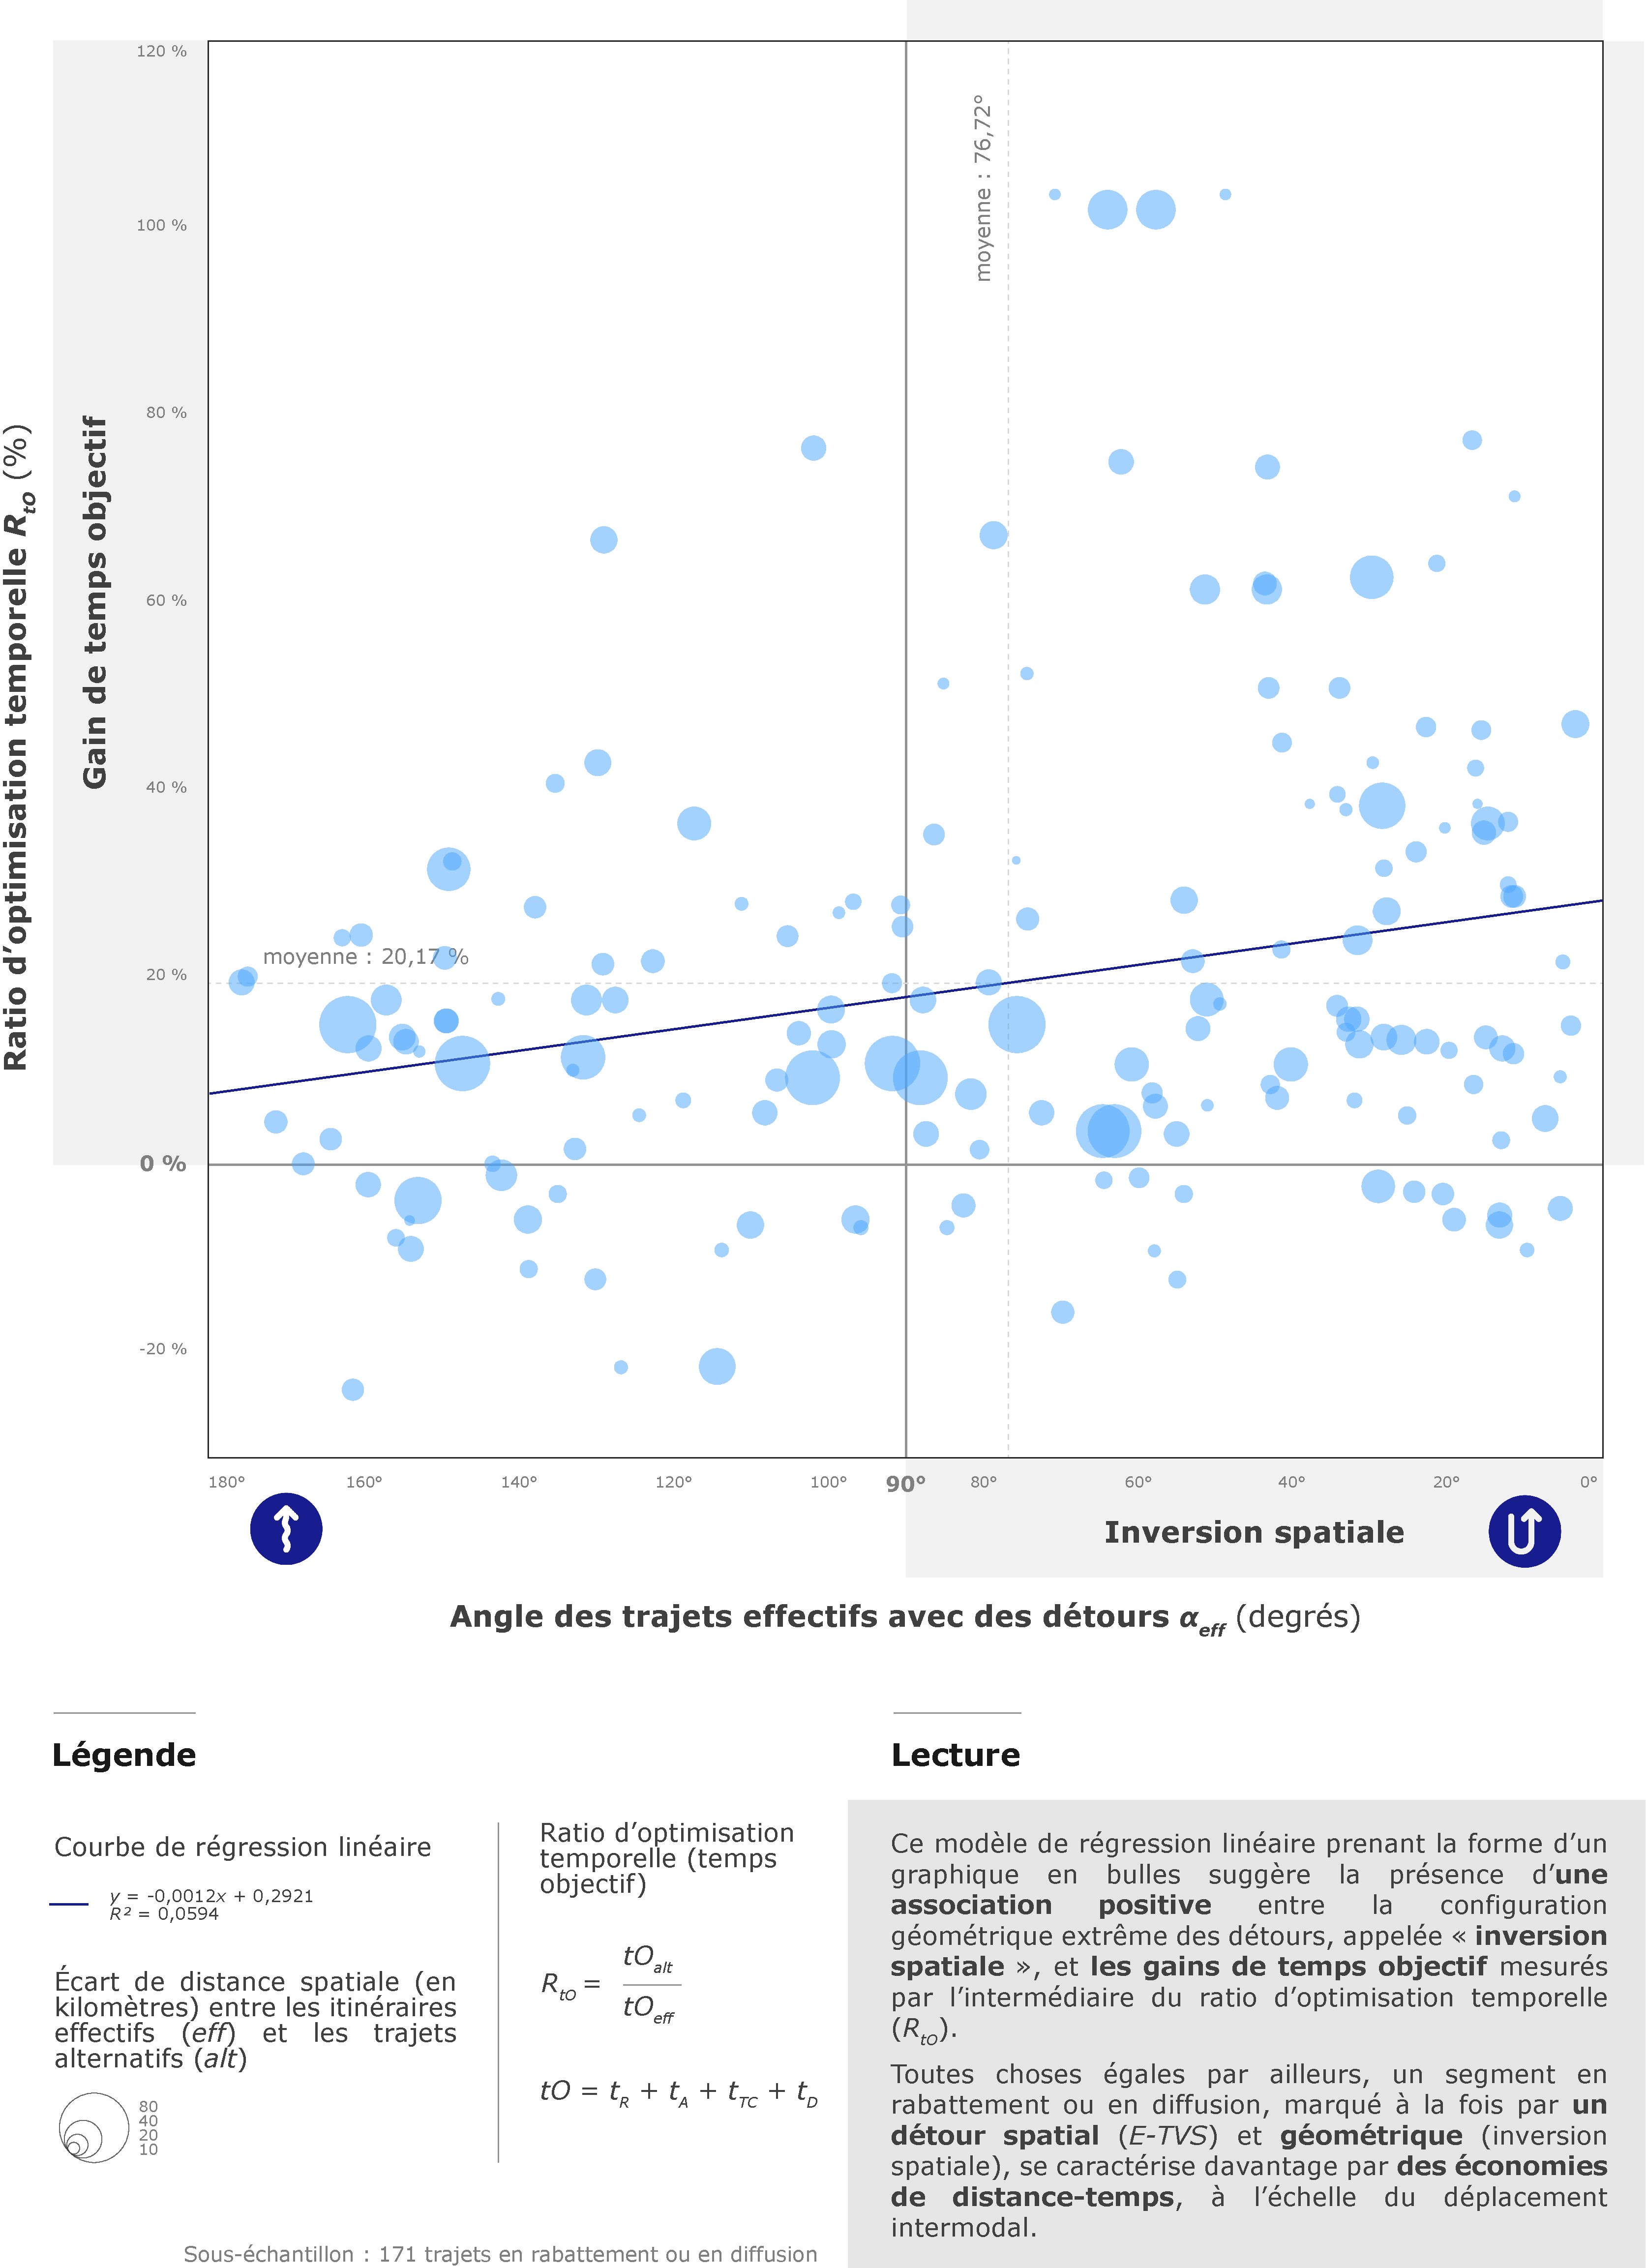
\includegraphics[width=1\columnwidth]{src/Figures/Chap-5/FR_Detours_Ratios_angles.pdf}}
        \vspace{5pt}
        \begin{flushright}\scriptsize{
        Auteur~: \textcolor{blue}{Dylan Moinse (2023)}
        %\\
        %Réalisation avec \Marque{Python}~et sur \Marque{Illustrator}
        }\end{flushright}
    \end{figure}

    % Egress
Dans ce contexte, les résultats statistiques suggèrent une propension accrue des usager·ère·s à opter pour des détours plus importants lors de leurs trajets en post-acheminement. Cette distinction entre les parcours en rabattement et en diffusion pourrait s'expliquer en partie par les variations de la \gls{perception} individuelle du temps entre les différentes phases d'un déplacement intermodal. À ce titre, l'étude publiée par \textcolor{blue}{\textcite[79]{schakenbos_valuation_2016}}\index{Schakenbos, Rik|pagebf}\index{La Paix Puello, Lissy|pagebf}\index{Nijënstein, Sandra|pagebf}\index{Geurs, Karst~T.|pagebf} souligne un rapport différent au coût associé à la correspondance en bus entre le trajet en rabattement, de l'ordre de treize minutes, et en diffusion, réduit à six minutes. Parallèlement, \textcolor{blue}{\textcite[3]{romm_differences_2022}}\index{Romm, Daniel|pagebf}\index{Verma, Priyanka|pagebf}\index{Karpinski, Elizabeth|pagebf}\index{Sanders, Tracy~L.|pagebf}\index{McKenzie, Grant|pagebf} ont démontré que les stations proches des terminus des lignes de métro à Boston enregistrent une activité potentielle de vélopartage plus importante pour le segment lié aux derniers kilomètres, tandis que les stations situées en centre urbain manifestent une plus grande activité pour les premiers kilomètres.%%Rédigé%%

    % Parcours commentés
La question de l'inversion spatiale apparaît revêtir un rôle essentiel dans les choix modaux effectués par les voyageur·se·s. Au travers d'un parcours commenté réalisé en \acrshort{TEP} et en \acrshort{TER}, des échanges avec la participante \(PCTE_{1}\) se référant à l'inversion spatiale peuvent être cités. Cette dernière a exprimé une préférence marquée pour l'usage de la trottinette électrique pour rejoindre la gare Lille Flandres, malgré la présence d'une ligne de métro traversant son quartier et desservant directement la gare en seulement deux arrêts. La première raison évoquée par cette usagère concerne la crainte de perturbations sur les réseaux de transport en commun urbain, susceptible de la contraindre à manquer son \acrshort{TER}, dont la fréquence est faible. Toutefois, un aspect géographique vient s'ajouter à cette considération. En effet, l'emplacement de la station de métro la plus proche de son domicile, l'arrêt Saint-Maurice Pellevoisin (ligne 2 du réseau \textsl{Ilévia}), se trouve, selon ses termes, \Guillemets{dans le sens opposé de la gare}~[12:18, \(PCTE^{TC}_{1}\)], comme l'illustre l'\hyperref[fig-chap5:pcte1a-inversion-spatiale]{extrait vidéo~\ref{fig-chap5:pcte1a-inversion-spatiale}} (page~\pageref{fig-chap5:pcte1a-inversion-spatiale}). La participante exprime ainsi le sentiment d'une perte de temps induite par la forme géométrique de l'itinéraire pour accéder à la ligne de métro. \Guillemets{\textsl{~C'est bête}, mais j'ai l'impression de perdre du temps en faisant demi-tour pour aller au métro\dots}~[12:18, \(PCTE^{TC}_{1}\)] nous confie-t-elle. Il est intéressant de noter que cette réflexion liée au choix modal de la trottinette au détriment du métro concerne exclusivement le trajet en pré-acheminement, de son domicile vers son lieu de travail. La participante paraît moins consciente de la présence d'une telle inversion spatiale lors de son trajet en post-acheminement, depuis la gare de Maubeuge. Ce constat met en lumière une tendance à privilégier la mobilité individuelle pour des trajets plus directs vers les stations de transport en commun, notamment pour les rejoindre, de manière à bénéficier d'itinéraires plus directs. Les usager·ère·s sont ainsi amené·e·s à opérer des détours, soit en vue d'obtenir des tracés géométriques plus directs, soit au contraire pour accéder à des systèmes de transport public plus performants en suivant une inversion spatiale.%%Rédigé%%

   %% Figure 1 Parcours commentés PCTE1A
    \begin{figure}[h!]\vspace*{4pt}
        \caption{Image extraite de l'itinéraire filmé en rabattement vers la gare Lille Flandres et illustrant une situation d'inversion spatiale (\(PCTE^{A}_{1}\)).}
        \label{fig-chap5:pcte1a-inversion-spatiale}
        \centerline{\includegraphics[width=1\columnwidth]{src/Figures/Chap-5/FR_Detours_PCTE1_Access_1.jpg}}
        \vspace{5pt}
        \begin{flushright}\scriptsize{
        Auteur~: \textcolor{blue}{Dylan Moinse (2022)}
        }\end{flushright}
    \end{figure}

    % 5.3.3.4.
    \needspace{1\baselineskip} % Réserve de l'espace
\subsubsection*{Typologie des stratégies d'optimisation basées sur les détours et les pauses
    \label{chap5:typologie-strategies-optimisation}
    }
 
    % Classification détours
L'analyse statistique des navetteur·se·s interrogé·e·s a été complétée par une analyse géostatistique des itinéraires \acrshort{E-TVS}, ce qui a permis d'identifier différentes catégories de stratégies d'optimisation basées premièrement sur les détours. Nous avons élaboré une classification des trois principaux types de détours identifiés, en fonction du contexte dans lequel la recherche d'optimisation spatio-temporelle du mouvement se manifeste, conformément à la \hyperref[fig-chap5:classification-strategies-optimisation-detours]{carte~\ref{fig-chap5:classification-strategies-optimisation-detours}} (page~\pageref{fig-chap5:classification-strategies-optimisation-detours}). Le premier type de comportement de mobilité est désigné sous le nom (i) d'\Guillemets{évitement des correspondances}, la seconde (ii) de \Guillemets{station de transport en commun plus attractive}~et la dernière (iii) de \Guillemets{réduction du temps à bord des transports en commun}.%%Rédigé%%

    % Méthodologie
La démarche analytique retenue pour classifier les itinéraires intermodaux intégrant des détours s'est fondée sur l'évaluation de plusieurs dimensions critiques~: (i) les distances spatiales et temporelles effectuées, (ii) le nombre total de correspondances nécessaires, (iii) la fréquence du service offert par le réseau de transport en commun, ainsi que (iv) la durée d'attente en station.%%Rédigé%%

   %% Figure corrélation angles et ratio temps
    \begin{carte}[h!]\vspace*{4pt}
        \centerline{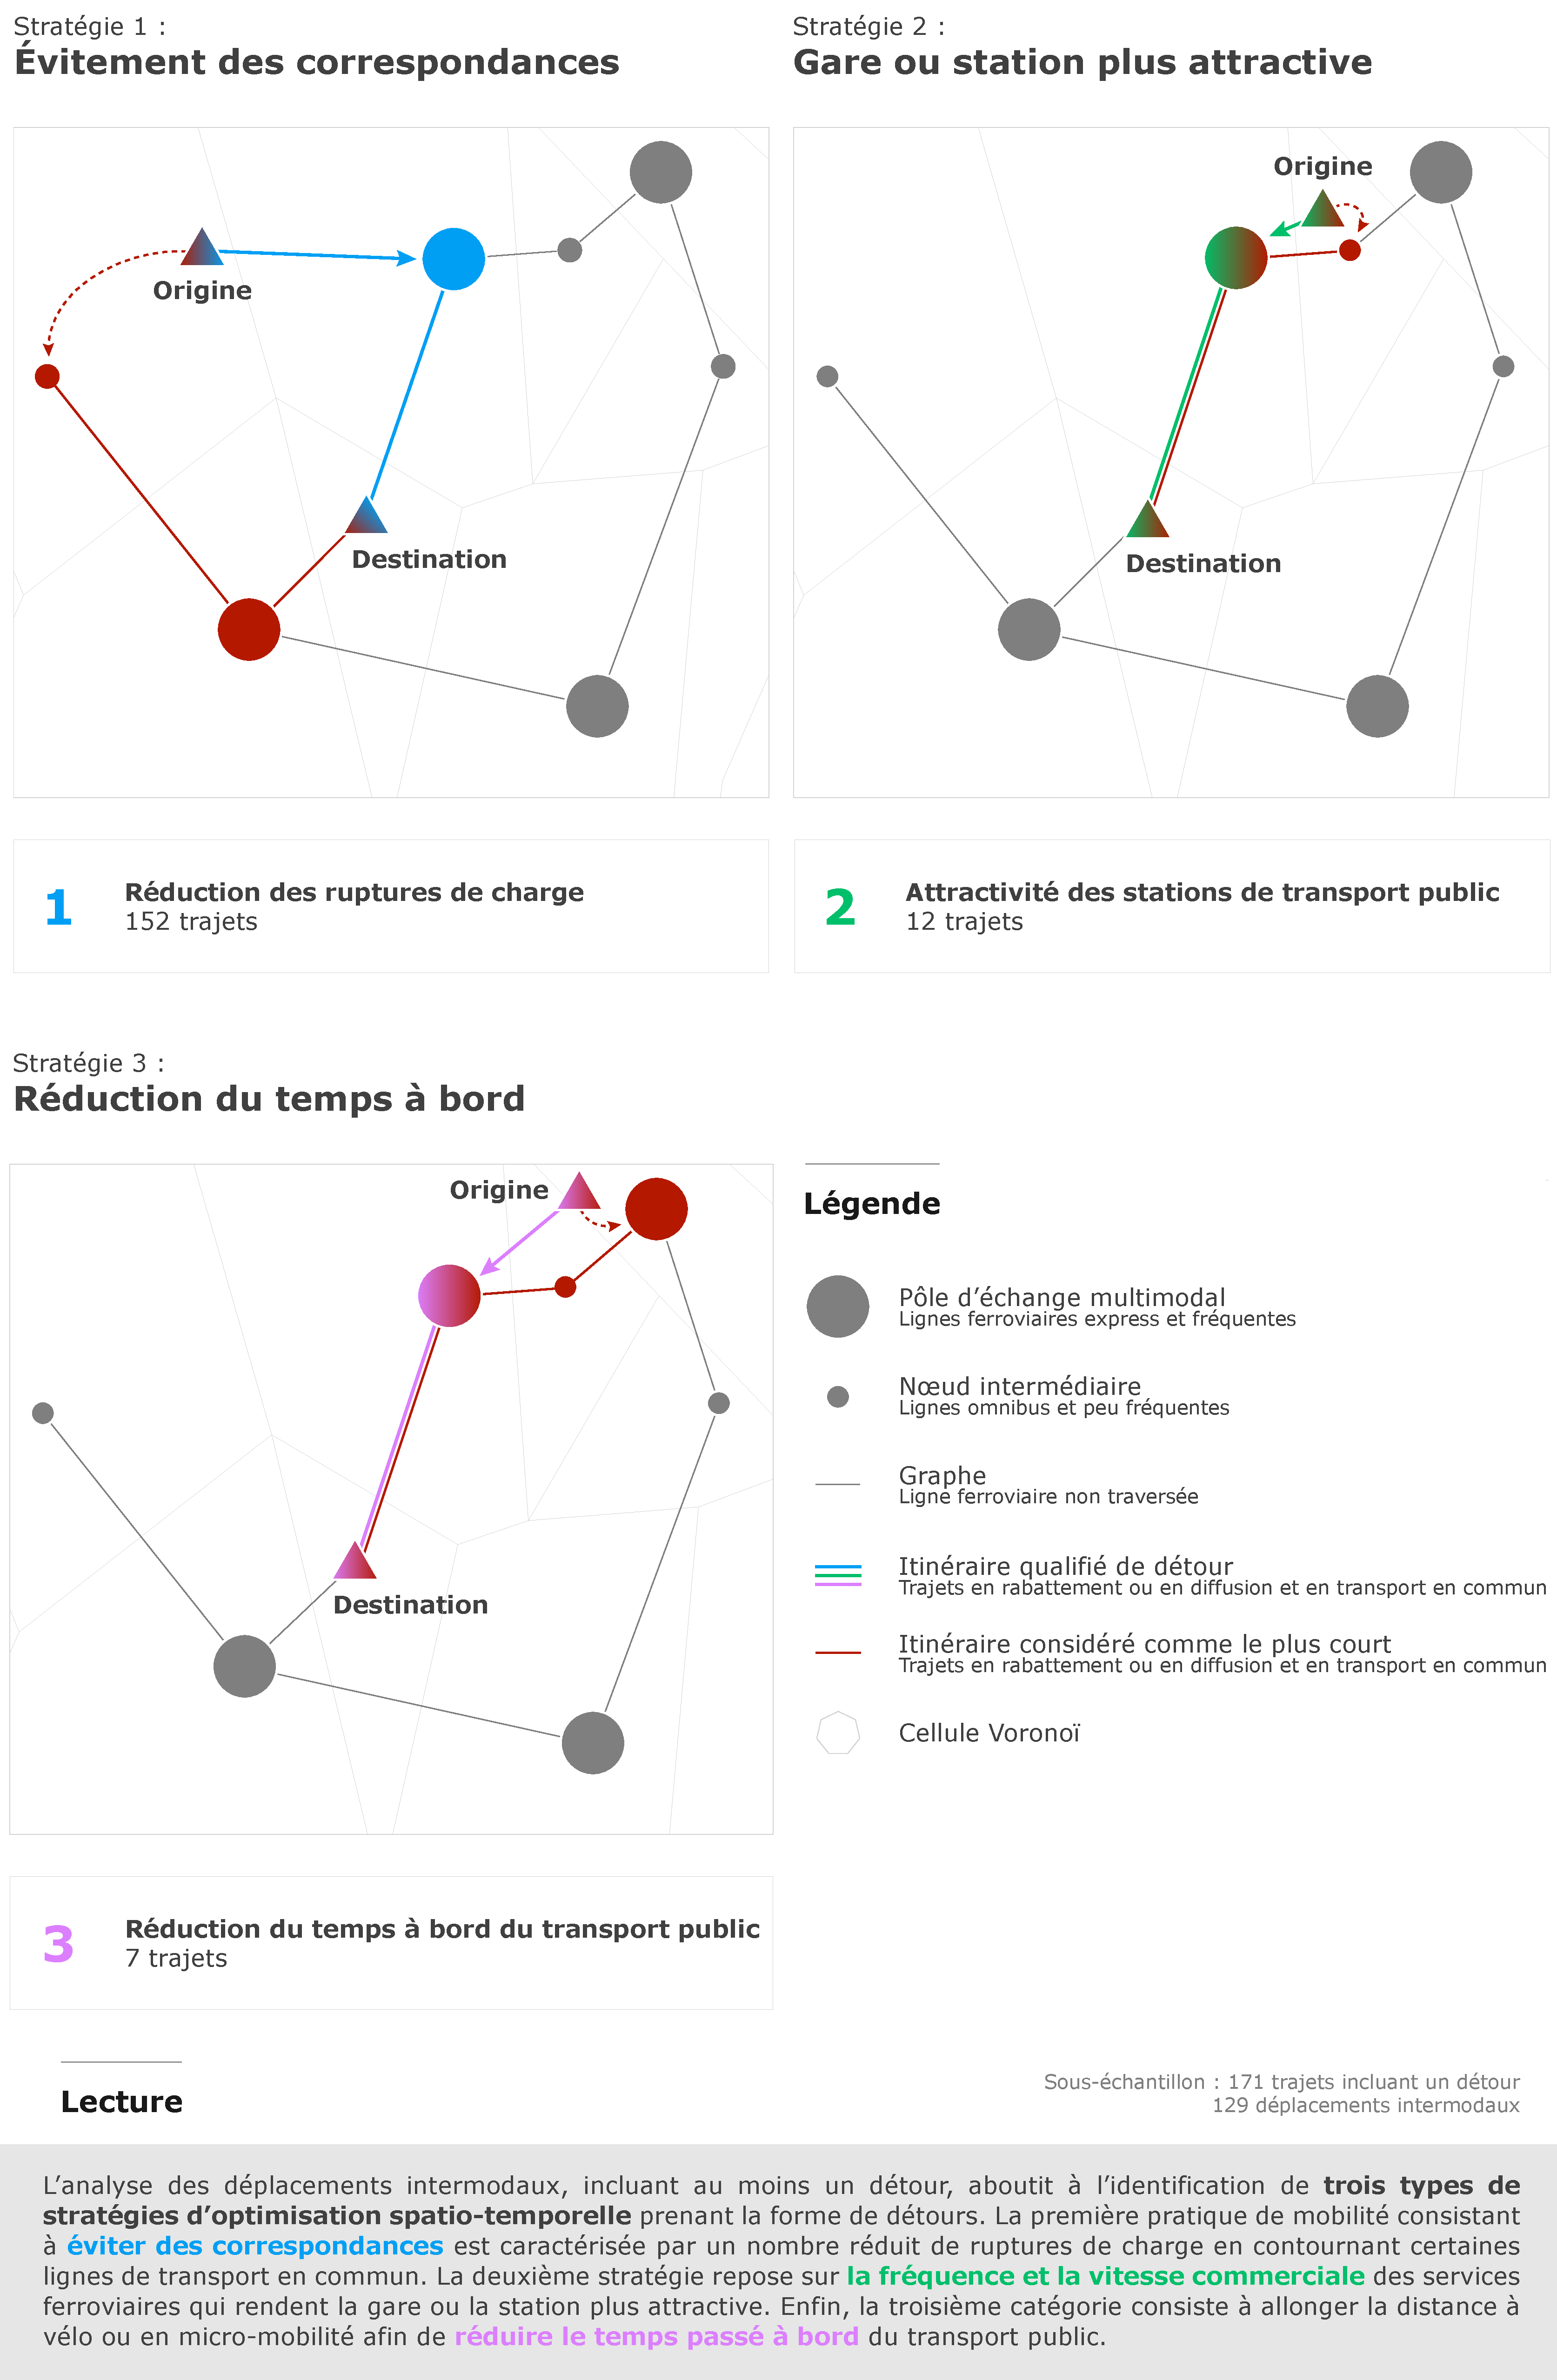
\includegraphics[width=1\columnwidth]{src/Figures/Chap-5/FR_Detours_Typologie.pdf}}
        \caption{Classification des stratégies d'optimisation intégrant des détours au sein des déplacements intermodaux.}
        \label{fig-chap5:classification-strategies-optimisation-detours}
        \vspace{5pt}
        \begin{flushright}\scriptsize{
        Auteur~: \textcolor{blue}{Dylan Moinse (2023)}
        }\end{flushright}
    \end{carte}

    % Méthode de classification
L'établissement de cette typologie des détours s'appuie sur plusieurs caractéristiques des déplacements \acrshort{E-TVS} analysées sur \Marque{QGIS}. Les variables examinées incluent les distances-temps et spatiales effectives à vélo ou en micro-mobilité et en transport en commun, le nombre total de ruptures de charge au cours du déplacement, la fréquence de chaque mode de déplacement utilité, ainsi que le temps d'attente lié à une correspondance. La première stratégie déterminée, l'\Guillemets{évitement des correspondances}, intervient lorsque le déplacement effectif comporte moins de correspondances que le déplacement alternatif. La catégorie liée aux \Guillemets{stations de transport en commun plus attractives}~se réfère au fait que l'usager·ère·s favorise une station de transport public dont la fréquence est plus élevée ou qui permet d'accéder à un système plus rapide en termes de vitesse commerciale. Enfin, la dernière stratégie correspondant à la \Guillemets{réduction du temps à bord des transports en commun}~est retenue lorsque le temps objectif dépensé dans le réseau de transport en commun est réduit aux dépens de la distance-temps à vélo ou en micro-mobilité. Il convient de noter que cette typologie considère l'échelle de chaque trajet effectué à l'aide de ces modes de déplacement légers afin d'identifier sur quel segment ces trois stratégies d'optimisation basées sur les détours sont mises en œuvre.%%Rédigé%%

    % Description typologie
Les trois stratégies d'optimisation définies à partir des détours observés dans le cadre de cette enquête se caractérisent de la manière suivante~:
\begin{enumerate}
    \item La stratégie d'\Guillemets{évitement des correspondances}~repose sur le désir de contourner une ligne de transport en commun, en accédant à une station plus éloignée, dans le but d'éviter une ou plusieurs correspondances. Cette pratique de mobilité réduit également les temps d'attente associés, souvent perçus de manière négative. Ce choix permet aussi au·à la voyageur·se d'éviter d'acquitter le prix du transport urbain. Cette première stratégie se traduit en moyenne par un trajet, en rabattement ou en diffusion, neuf minutes plus long pour les cyclistes désireux·ses d'éviter une rupture de charge. La stratégie visant à réduire les temps de correspondance au prix d'un allongement de la durée totale de transport est conforme à la pondération utilisée en économétrie des transports vis-à-vis de ces durées perçues très négativement par les voyageur·se·s. Cette stratégie d'optimisation a été identifiée dans 152 des 171 segments en rabattement et en diffusion. Dans la moitié des cas, ces détours correspondent à l'évitement d'une ligne de métro~;
    \item La stratégie consistant à favoriser une \Guillemets{station de transport en commun plus attractive}~repose sur le fait de privilégier une station offrant un meilleur niveau de service (\textsl{Level of Service}, LOS) par rapport à la station la plus proche du lieu d'origine ou de destination, mais sans réduire le nombre de correspondances. Dans la majorité des situations observées, cette pratique de mobilité permet non seulement de bénéficier d'une fréquence de trains plus élevée, mais également de trains plus rapides. Cette stratégie d'optimisation a été identifiée dans douze trajets en rabattement et en diffusion~;
    \item La stratégie visant une \Guillemets{réduction du temps à bord des transports en commun}~implique l'accès à une station de transport en commun plus éloignée, offrant pourtant un service de qualité équivalente à la station la plus proche, afin de réduire le temps passé dans les transports en commun. Seuls sept trajets ont été classés dans cette stratégie d'optimisation basée sur les détours.
\end{enumerate}%%Rédigé%%

    % Discussion typologie détours
Cette typologie des détours empruntés par les voyageur·se·s intermodaux·les conforte plusieurs contributions présentes dans la littérature scientifique. À La Haye, \textcolor{blue}{\textcite[3]{rijsman_walking_2019}}\index{Rijsman, Lotte|pagebf}\index{Molin, Eric|pagebf}\index{Teijl, Thomas|pagebf}\index{Oort, Niels van|pagebf}\index{Ton, Danique|pagebf}\index{Hoogendoorn, Serge|pagebf} ont effectivement conclu que les motifs expliquant le choix d'un arrêt de transport en commun plus éloigné par les piéton·ne·s sont principalement liés à la volonté d'éviter une correspondance, et dans une moindre mesure à la qualité et au confort du service de transport. En parallèle, \textcolor{blue}{\textcite[468]{jonkeren_bicycle-train_2021}}\index{Jonkeren, Olaf|pagebf}\index{Kager, Roland|pagebf}\index{Harms, Lucas|pagebf}\index{te Brömmelstroet, Marco|pagebf} et \textcolor{blue}{\textcite[2144]{krizek_bicycling_2010}}\index{Krizek, Kevin~J.|pagebf}\index{Stonebraker, Eric~W.|pagebf} mettent en évidence le rôle des stations de transport les plus attractives et confortables aux Pays-Bas. Notre analyse géostatistique révèle également un temps mesuré supplémentaire de neuf minutes pour la première stratégie d'optimisation, basée sur l'évitement des correspondances, en accord avec la documentation à ce sujet. L'étude néerlandaise de \textcolor{blue}{\textcite[665]{mil_insights_2020}}\index{Mil, Joeri~F.P. van|pagebf}\index{Leferink, Tessa~S.|pagebf}\index{Annema, Jan Anne|pagebf}\index{Oort, Niels van|pagebf} souligne une préférence pour une distance-temps supplémentaire de cinq à dix minutes à vélo pour réduire le nombre de correspondances. Par ailleurs, \textcolor{blue}{\textcite[143]{kampen_bicycle_2021}}\index{Kampen, Jullian van|pagebf}\index{Knapen, Luk|pagebf}\index{Pauwels, Eric|pagebf}\index{Mei, Rob van der|pagebf}\index{Dugundji, Elenna~R.|pagebf} et \textcolor{blue}{\textcite{kampen_understanding_2021}}\index{Kampen, Jullian van|pagebf}\index{Jayaraj, Manoj Ashvin|pagebf}\index{Pauwels, Eric|pagebf}\index{Mei, Rob van der|pagebf}\index{Dugundji, Elenna~R.|pagebf} démontrent que les cyclistes intermodaux·les, dans le Grand Amsterdam, préfèrent se rendre vers la seconde gare la plus proche si la durée du déplacement en train est plus raccourcie ou afin d'éviter un transfert, principalement s'agissant des voyageur·se·s de moins de 39 ans et disposant d'un revenu mensuel net inférieur à 2~500€. De plus, ces enseignements peuvent résonner avec d'autres types de déplacements qui ne rentrent pas dans le cadre de cette recherche doctorale, tels que les déplacements \Guillemets{non dirigés} (\textsl{undirected trips}) qui contribuent à un niveau de satisfaction personnelle accru, comme en témoigne le travail de \textcolor{blue}{\textcite[8-9]{hook_undirected_2021}}\index{Hook, Hannah|pagebf}\index{Vos, Jonas de|pagebf}\index{Acker, Veronique van|pagebf}\index{Witlox, Frank|pagebf} sur les promenades réalisées dans les Flandres, en Belgique, qui tendent à être plus longs et à être corrélés positivement avec le bien-être, notamment puisqu'ils nécessitent davantage d'activité physique.%%Rédigé%%

    % Typologie pauses
Un second aspect lié aux stratégies d'optimisation réside dans la \gls{pause} qui survient nécessairement lors du changement de mode de déplacement, notamment en rejoignant et en sortant d'un système de transport en commun, s'agissant des déplacements intermodaux. Ce temps intermédiaire lié à l'attente du transport public peut être analysé comme une opportunité pour optimiser la chaîne de déplacement, mais aussi comme une occasion de réaliser des activités supplémentaires au cours du déplacement. Les 110 répondant·e·s qui ont déclaré avoir réalisé une activité pendant leur temps d'attente en gare ont été invités à préciser les types d'activités favorisés, à l'aide d'une question à choix multiples suivie d'une réponse libre. L'analyse de l'optimisation spatio-temporelle par la pause démontre qu'une majorité des pauses a été utilisée comme un moment propice pour effectuer des achats, tandis qu'un quart des répondant·e·s déclarent profiter des temps de pause pour entretenir des interactions sociales ou pour réaliser des activités professionnelles (voir le \hyperref[table-chap5:motifs-pauses]{tableau~\ref{table-chap5:motifs-pauses}}, page~\pageref{table-chap5:motifs-pauses}). Plus précisément, les voyageur·se·s ont principalement indiqué textuellement que le motif secondaire lié aux achats concerne essentiellement les achats alimentaires, tandis que les motifs liés aux rencontres sociales et aux activités professionnelles dépendent principalement de l'accompagnement des enfants et de temps productif associé au travail.%%Rédigé%%

    % Tableau Typologie pauses
% Tableau Typologie pauses
%%Rédigé%%
        \begin{table}[h!]
        \centering
        \renewcommand{\arraystretch}{1.5}
        \resizebox{\columnwidth}{!}{
        \begin{tabular}{p{0.58\columnwidth}p{0.21\columnwidth}p{0.21\columnwidth}}
        %\hline
    \rule{0pt}{15pt} \textcolor{blue}{\textbf{Typologie des pauses}} & \textcolor{blue}{\textbf{Effectif}} & \textcolor{blue}{\textbf{Part}}\\
        \hline
\small{Achats} & \small{82} & \small{74,5~\%} \\
\small{Rencontres sociales et accompagnement} & \small{30} & \small{27,3~\%} \\
\small{Activités professionnelles} & \small{27} & \small{24,5~\%} \\
\small{Loisirs} & \small{23} & \small{20,9~\%} \\
\small{Tâches administratives} & \small{17} & \small{15,5~\%} \\
\small{Visites et promenades} & \small{16} & \small{14,5~\%} \\
        \hline
        \end{tabular}}
    \caption{Raisons avancées pour les 110 pauses déclarées, lors des déplacements intermodaux, par les cyclo-voyageur·se·s.}
    \label{table-chap5:motifs-pauses}
        \vspace{5pt}
        \begin{flushleft}\scriptsize{
        \textcolor{blue}{Note~:} la question concernée étant à choix multiples, la part totale est supérieure à 100~\%.
        \\
        \textcolor{blue}{Lecture~:} les achats constituent la principale raison des pauses lors des déplacements intermodaux, suivis des rencontres sociales et de l'accompagnement, et des activités professionnelles. Ce tableau souligne ainsi la diversité des motifs associés aux interruptions de parcours.
        }\end{flushleft}
        \begin{flushright}\scriptsize{
        Auteur~: \textcolor{blue}{Dylan Moinse (2023)}
        }\end{flushright}
        \end{table}%%Rédigé%%

    %% Parcours commentés
Les observations tirées de cette analyse statistique s'accordent avec les pratiques rapportées par la participante désignée sous le nom de \(PCTE_{1}\), interviewée au cours d'un déplacement intégrant à la fois l'usage d'une trottinette électrique et du \acrshort{TER}. Cette usagère a partagé son expérience relative à certaines de ses pratiques d'achats alimentaires, habituellement effectués lors de son trajet retour vers son domicile, en particulier à la gare Lille Flandres, qui constitue son point d'arrivée en sens inverse. Elle indique s'arrêter fréquemment à cette gare afin de bénéficier des commodités et des services commerciaux disponibles au sein de ce pôle multimodal, incluant, à titre d'exemple, une boulangerie (voir l'\hyperref[fig-chap5:pcte1a-commerces-lille-flandres]{extrait vidéo~\ref{fig-chap5:pcte1a-commerces-lille-flandres}}, page~\pageref{fig-chap5:pcte1a-commerces-lille-flandres}). Toutefois, elle soulève un point de gêne concernant l'introduction de sa trottinette dans les espaces commerciaux. Face à la suggestion d'établir un espace de stationnement gratuit et réservé aux \acrshort{EDPM} au sein des gares, la participante exprime un intérêt conditionnel, dépendant du contexte et de la nature de ses achats~: \Guillemets{Tout dépend du type d’achat. Si c’est pour passer du temps, mais si c’est seulement pour acheter une baguette de pain, je l’utiliserai pas. Car le temps de ranger la trottinette et de jongler avec les cartes d'abonnement\dots Si je dois faire deux ou trois magasins, pourquoi pas}~[10:36, \(PCTE^{TC}_{1}\)].%%Rédigé%%
    
   %% Figure 2 Parcours commentés PCTE1A
    \begin{figure}[h!]\vspace*{4pt}
        \caption{Image extraite de l'itinéraire filmé en rabattement vers la gare Lille Flandres et faisant apparaître la gare accueillant certains commerces (\(PCTE^{A}_{1}\)).}
        \label{fig-chap5:pcte1a-commerces-lille-flandres}
        \centerline{\includegraphics[width=1\columnwidth]{src/Figures/Chap-5/FR_Detours_PCTE1_Access_13.jpg}}
        \vspace{5pt}
        \begin{flushright}\scriptsize{
        Auteur~: \textcolor{blue}{Dylan Moinse (2022)}
        }\end{flushright}
    \end{figure}

    % Discussion temps équipé
La conception du temps consacré aux déplacements a subi une évolution notable dans la recherche contemporaine, notamment en ce qui concerne son utilisation dans les transports en commun. Perçu majoritairement comme une contrainte subie ou une désutilité, le temps passé dans les transports est désormais considéré par certain·e·s économistes comme une opportunité d'optimisation et de valorisation des activités quotidiennes. Cette réévaluation s'inscrit dans une perspective où le temps de transport n'est plus uniquement envisagé comme une perte, mais comme une ressource pouvant être exploitée de manière productive. D'après les travaux de \textcolor{blue}{\textcite[28]{joly_rapports_2003}}\index{Joly, Iragaël|pagebf}, cette valorisation s'inscrit dans une quête plus large de l'espace et du confort, amenant les individus à accepter un investissement temporel dans les transports. Les stratégies individuelles d'optimisation du temps à bord des transports en commun, étudiées par \textcolor{blue}{\textcite[85]{jain_gift_2008}}\index{Jain, Juliet|pagebf}\index{Lyons, Glenn|pagebf}, traduisent une volonté de rendre ce temps utile, que ce soit à travers des activités professionnelles ou liées aux loisirs. Dans cette optique, les modes de déplacement passifs, tels que les transports en commun, deviennent des espaces dans lesquels s'exerce une certaine productivité \textcolor{blue}{\autocite[115]{lyons_use_2007}}\index{Lyons, Glenn|pagebf}\index{Jain, Juliet|pagebf}\index{Holley, David|pagebf}. Le temps de déplacement est alors exploité pour des activités variées, allant du travail aux loisirs tels que la lecture ou l'écoute de musique, contribuant ainsi au bien-être et à l'épanouissement personnel \textcolor{blue}{\autocite[17]{moinse_temps_2020}}\index{Moinse, Dylan|pagebf}. Toutefois, la valorisation de ce temps est conditionnée par divers facteurs tels que le confort, l'ergonomie, l'accessibilité et la connaissance du réseau, voire la connectivité au réseau de communication \textcolor{blue}{\autocite[21]{bounie_what_2019}}\index{Bounie, Nathan|pagebf}\index{Adoue, François|pagebf}\index{Koning, Martin|pagebf}\index{L'Hostis, Alain|pagebf}. Le \Guillemets{temps équipé}, ou \textsl{equipped time} \textcolor{blue}{\autocite[87]{jain_gift_2008}}\index{Jain, Juliet|pagebf}\index{Lyons, Glenn|pagebf}, illustre un avantage compétitif des systèmes de transport en commun en offrant un temps disponible pour diverses activités, en ce qui concerne non seulement les déplacements pendulaires, mais également ceux dédiés aux loisirs \textcolor{blue}{\autocite[111]{lyons_use_2007}}\index{Lyons, Glenn|pagebf}\index{Jain, Juliet|pagebf}\index{Holley, David|pagebf}. Dans ce contexte, les mobilités émergentes telles que la voiture autonome présentent un défi pour le transport public. En offrant une autonomie similaire à celle des transports en commun, ces nouvelles formes de mobilité pourraient remettre en question leur compétitivité. En outre, ce phénomène pourrait créer un paradoxe avec la promotion des mobilités actives, dans la mesure où le \Guillemets{temps équipé} favorise les modes de déplacement moins actifs\footnote{
    \textcolor{blue}{\textcite[21]{bounie_what_2019}}\index{Bounie, Nathan|pagebf}\index{Adoue, François|pagebf}\index{Koning, Martin|pagebf}\index{L'Hostis, Alain|pagebf} ont mesuré, à l'aide d'un modèle logit ordinal, les effets de l'usage du \textsl{smartphone} et de la connexion mobile sur la réduction des contraintes spatio-temporelles rencontrées à bord du métro parisien. Leur analyse a démontré que la perception de la valeur du temps de trajet diminue de 12~\% lorsque les usager·ère·s disposent d'une connectivité aux réseaux mobiles durant leur voyage.
}.%%Rédigé%%

    % Discussion pauses
La possibilité de mener ces activités dépend grandement de l'existence d'un temps de pause et de sites d'activité et de services situés dans ou à proximité de la gare ferroviaire. Cette analyse met en lumière le rôle positif des pauses dans les trajets intermodaux, soulignant la contribution des commodités urbaines à la formation de distances optimales et, par conséquent, de trajets optimaux, dans le cadre de l'objectif plus vaste de favoriser des alternatives à la voiture pour la mobilité à l'échelle régionale. Cette connexion entre les enjeux de transport et de développement urbain appelle à une attention renouvelée de la part des acteurs urbains et du transport en ce qui concerne la conception des gares ferroviaires et de leur environnement, ainsi que la distribution des services. Cela s'inscrit dans la lignée de l'étude menée par \textcolor{blue}{\textcite[468]{jonkeren_bicycle_2021}}\index{Jonkeren, Olaf|pagebf}\index{Kager, Roland|pagebf}, qui montre que la visite de supermarchés et d'autres magasins est l'activité la plus fréquente pour le chaînage de déplacements sur la portion d'accès à vélo.%%Rédigé%%

    % 5.3.3.5.
    \needspace{1\baselineskip} % Réserve de l'espace
\subsubsection*{Clustérisation des déplacements intermodaux \acrshort{E-TVS} du point de vue de l'optimisation spatio-temporelle
    \label{chap5:clusterisation-detours}
    }

    % Type d'analyse
En procédant à l'estimation des différents ratios d'optimisation (\(R\)), l'analyse statistique cherche à regrouper les déplacements intermodaux en fonction des gains de distance mesurés. Pour cela, nous avons mis en perspective le coefficient d'optimisation spatiale (\(R_{km}\)) et le coefficient d'optimisation temporelle perçue (\(R_{t_{(P)}}\)) afin de répartir les itinéraires au regard des deux variables mobilisées. D'une part, le ratio d'optimisation spatiale se réfère aux gains de distance spatiale réalisés en confrontant la distance spatiale effective (\(km_{eff}\)) avec la distance spatiale la plus courte possible, qualifiée d'alternative (\(km_{alt}\)). D'autre part, le ratio d'optimisation temporelle représente les gains de temps réalisés entre la distance temporelle ressentie et effective (\(t_{eff_{(P)}}\)) et alternative (\(t_{alt_{(P)}}\)). En fonction des valeurs obtenues pour \(R_{km}\) et \(R_{t_{(P)}}\), cette évaluation statistique positionne les déplacements \acrshort{E-TVS} analysés par rapport aux soldes spatiaux et temporels. De cette manière, l'analyse se présente sous la forme d'un graphique en bulles qui représente \(R_{t_{(P)}}\) en fonction de \(R_{km}\) (voir l'\hyperref[fig-chap5:profils-strategies-optimisation-detours]{illustration~\ref{fig-chap5:profils-strategies-optimisation-detours}}, page~\pageref{fig-chap5:profils-strategies-optimisation-detours}). Une troisième variable est également exposée dans la lecture statistique et est basée quant à elle sur la différence entre la distance spatiale des déplacements effectifs (\(km_{eff}\)) et celle des déplacements alternatifs (\(km_{alt}\)), tandis qu'une dernière variable catégorielle informe du type de stratégie d'optimisation concernée. Il convient de préciser que cette méthode d'analyse par clustérisation repose sur la notion de regroupement visuel, soit la détection de concentrations de points en fonction d'un graphique croisant diverses variables, et ne repose pas sur des algorithmes veillant à établir un regroupement avancé. Au contraire, cette approche représente une analyse préliminaire des types de cyclistes intermodaux·les qui optent pour des détours.%%Rédigé%%

   %% Figure clustérisation profils détours
    \begin{figure}[h!]\vspace*{4pt}
        \caption{Regroupement des déplacements intermodaux impliquant un détour selon les profils d'optimisation spatio-temporelle.}
        \label{fig-chap5:profils-strategies-optimisation-detours}
        \centerline{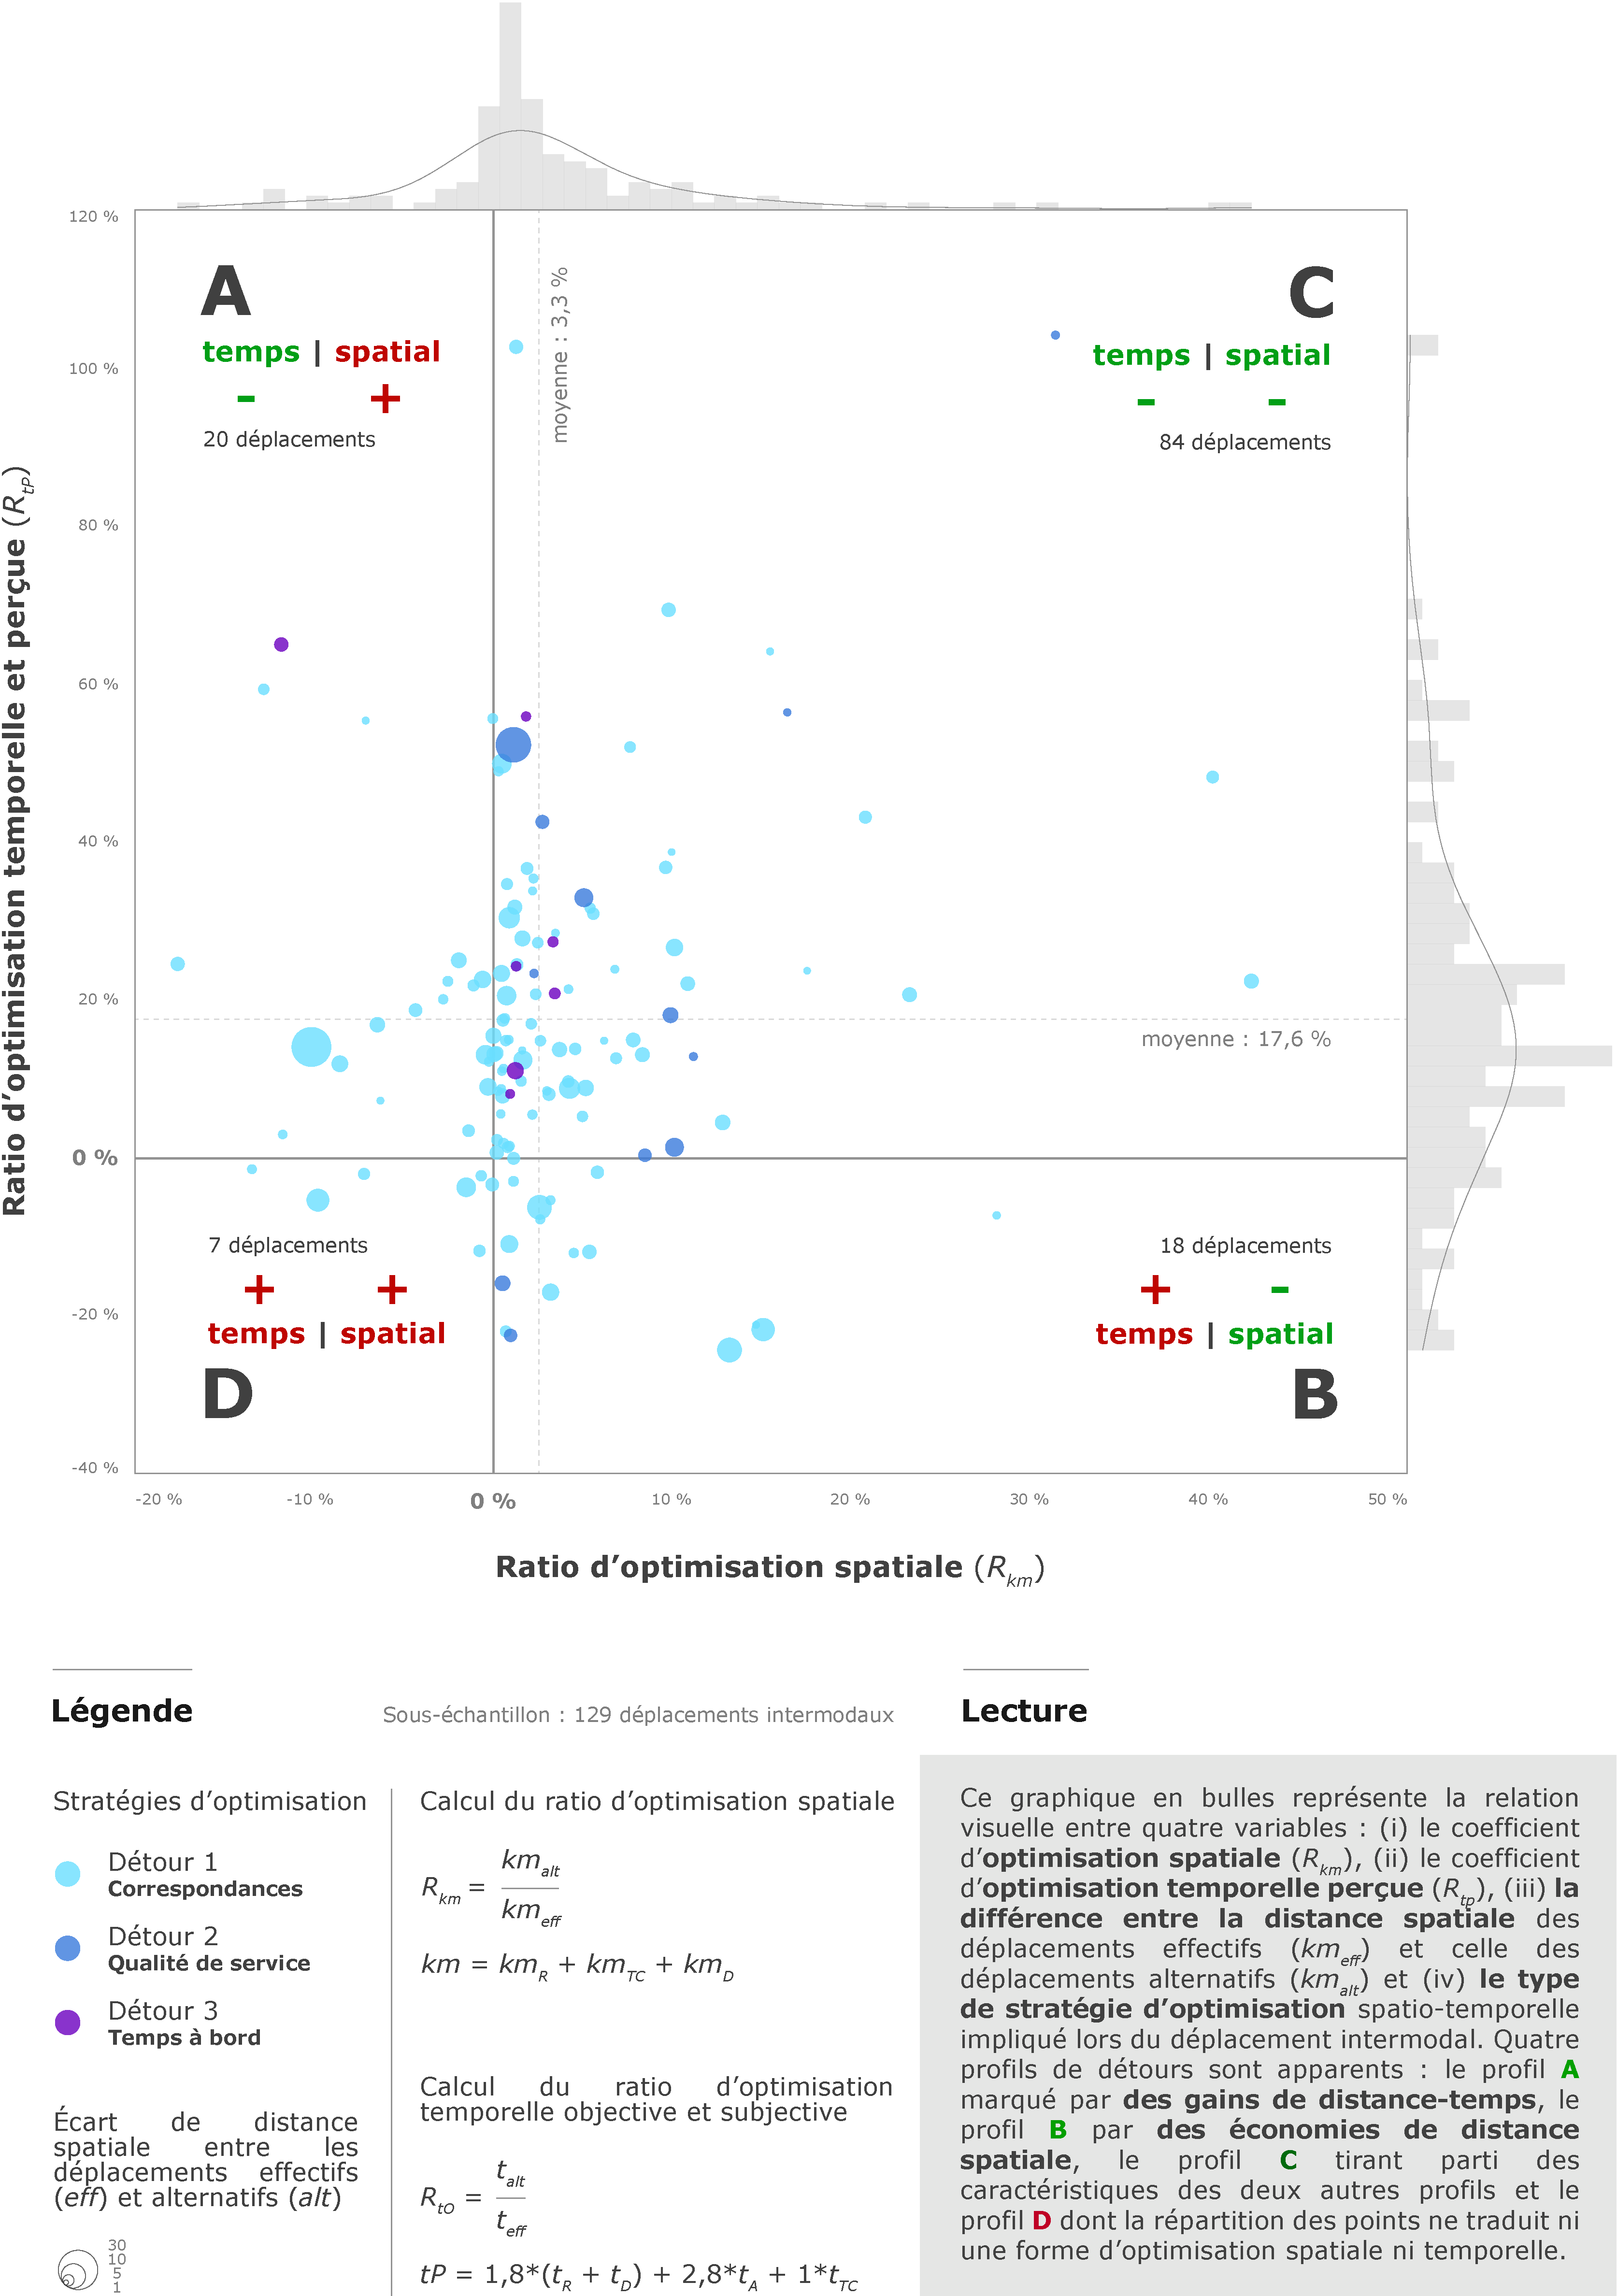
\includegraphics[width=1\columnwidth]{src/Figures/Chap-5/FR_Detours_Cluster_optimisation_detours.pdf}}
        \vspace{5pt}
        \begin{flushright}\scriptsize{
        Auteur~: \textcolor{blue}{Dylan Moinse (2023)}
        %\\
        %Réalisation avec \Marque{Python}~et sur \Marque{Illustrator}
        }\end{flushright}
    \end{figure}
    
    % Résultats
L'analyse statistique par regroupement des déplacements \acrshort{E-TVS} vise à mieux situer le rôle des détours dans la recherche d'optimisation spatio-temporelle. Cette approche met en évidence quatre profils de détours générateurs d'optimisation. Le profil \(A\) se caractérise par des économies de distance-temps, mais par un ratio de distance spatiale défavorable, tandis que le profil \(B\) privilégie les gains de distance spatiale au détriment de la distance-temps. En parallèle, le profil \(C\) combine les avantages en termes de distance-temps et spatiale, alors que le profil \(D\) cumule un ratio d'optimisation spatiale et temporelle négatif. La représentation graphique, telle qu'apparente dans l'\hyperref[fig-chap5:profils-strategies-optimisation-detours]{illustration~\ref{fig-chap5:profils-strategies-optimisation-detours}} (page~\pageref{fig-chap5:profils-strategies-optimisation-detours}), met en lumière un regroupement dense de 84 déplacements \acrshort{E-TVS} (65~\%) au sein du profil \(C\). De plus, en associant les profils \(A\), \(B\) et \(C\), nous pouvons constater que 95~\% des itinéraires analysés sont inclus. Ce résultat suggère que la quasi-totalité des détours étudiés assurent des économies de distance-temps et, ou bien, de distance spatiale par rapport aux itinéraires alternatifs. En revanche, la différence spatiale qui existe entre les itinéraires effectifs et alternatifs ne semble pas avoir d'effet simple sur les ratios d'optimisation spatio-temporelle, laissant supposer qu'un détour de faible proportion est à même, dans certaines conditions, d'optimiser significativement un déplacement intermodal.%%Rédigé%%

    % Transition
Cependant, l'examen de certains détours présents dans le profil \(D\), dont l'optimisation spatio-temporelle n'est pas démontrée, suggère que des facteurs exogènes, n'étant ni spatiaux ni temporels, pourraient justifier le choix de tels itinéraires.%%Rédigé%%

    % 5.3.4.
    \needspace{1\baselineskip} % Réserve de l'espace
\subsection{Regards croisés sur les détours, les pauses et l'optimisation
    \label{chap5:discussion-detours-pauses-optimisation}
    }

    % Introduction
Bien que cette recherche ait délibérément mis l'accent sur les dimensions liées à la distance, il demeure essentiel d'intégrer des variables fondamentales influençant les choix d'itinéraires dans le cadre des comportements de mobilité, telles que les caractéristiques de l'environnement urbain, la configuration des réseaux, ainsi que l'ambiance et les niveaux de stress associés aux pratiques intermodales intégrant l'usage du vélo et de la micro-mobilité \textcolor{blue}{\autocite[79]{zuo_incorporating_2021}}\index{Zuo, Ting|pagebf}\index{Wei, Heng|pagebf}\index{Chen, Na|pagebf}.%%Rédigé%%

    % 5.3.4.1.
    \needspace{1\baselineskip} % Réserve de l'espace
\subsubsection*{Influence de la valorisation des espaces publics sur les stratégies d'optimisation
    \label{chap5:environnement-urbain}
    }

    % Rôle environnement urbain (ID 145 Houchin à Loos-lez-Lille)
Considérant le rôle joué par l'environnement urbain, notamment le traitement des espaces publics et son impact sur le choix modal tel que présenté dans la \acrfull{RSL} du \hyperref[chap2:titre]{chapitre~2} (page~\pageref{chap2:titre}), nous avons fait le choix d'adopter une approche qualitative en nous appuyant sur une étude de cas issue du questionnaire administré. Cet exemple de déplacement intermodal déclaré a été retenu en rapport avec le contexte géographique dans lequel il s'inscrit. L'analyse spatiale de ce voyage, caractérisé par une stratégie d'optimisation spatio-temporelle incluant des détours, implique effectivement la \acrshort{CABBALR} et la \acrshort{MEL}. Le déplacement intermodal enquêté est ainsi réalisé sur le réseau ferroviaire classique entre la gare de Béthune et la halte Lille CHR, avec un lieu d'origine situé à Houchin, à environ quatre kilomètres de la gare de Béthune à vol d'oiseau, et un lieu de destination à Loos-lez-Lille, à environ deux kilomètres de la halte. Réalisé au moins cinq fois par semaine, ce déplacement implique l'utilisation de la voiture personnelle jusqu'à la première gare régionale, puis du train et de la \acrshort{TEP} depuis la gare intermédiaire. Il est à noter que le lieu de domicile de la répondante se trouve plus près de la gare de Nœux-les-Mines (3 kilomètres à vol d'oiseau) et que le lieu de destination est plus proche de la gare de Loos-lez-Lille (0,4 kilomètre), comme cartographié sur la \hyperref[fig-chap5:exemple-detours-lille-chr]{carte~\ref{fig-chap5:exemple-detours-lille-chr}} (page~\pageref{fig-chap5:exemple-detours-lille-chr}). Néanmoins, les détours effectués tant en pré-acheminement qu'en post-acheminement offrent à ce·tte voyageur·se un moyen d'optimiser son déplacement.%%Rédigé%%

    % Rabattement
Au sein du premier segment de déplacement jusqu'à la gare de Béthune, nous pouvons observer une stratégie visant à réduire la contrainte associée à une rupture de charge. Bien que la ligne ferroviaire reliant les gares de Béthune à Lille CHR soit directe, par le biais des trains K50 ou C50 reliant Saint-Pol-sur-Ternoise à Lille\footnote{
    \textcolor{blue}{\textcite[468]{sncf_voyageurs_trains_nodate}} désigne les différentes lignes de \acrshort{TER} mises en service en fonction du type de service et de la vitesse commerciale du train~: le \acrshort{TER} de type \Guillemets{KRONO} (\(K\)) assure des liaisons directes avec peu d'arrêts entre les pôles régionaux, le \acrshort{TER} de type \Guillemets{CITI} (\(C\)) assure des liaisons sur des distances moyennes autour des villes, tandis que le \acrshort{TER} de type \Guillemets{PROXI} (\(P\)) assure des liaisons dites de proximité. Il faut noter que cette classification peut différer en fonction des services et des régions.
}, le trajet depuis la gare de Nœux-les-Mines vers Lille exige une correspondance à Béthune. Dans un premier temps, l'usager·ère devrait alors utiliser, depuis la gare de Nœux-les-Mines, la ligne K52 reliant Arras à Dunkerque ou P54 entre Arras et Calais-ville à destination de Béthune, ou bien ces mêmes lignes dans le sens inverse à destination de Lens. Dans un second temps, l'usager·ère devrait rejoindre la ligne K50 ou C50 entre Saint-Pol-sur-Ternoise et Lille depuis la gare de Béthune ou bien la ligne K51 ou C51 entre Lens et Lille. Cependant, en parcourant cinq minutes supplémentaires en voiture personnelle au cours du trajet en pré-acheminement, le·la voyageur·se parvient directement à rejoindre la gare de Béthune, depuis son lieu d'origine situé à Houchin. Certes, le trajet en pré-acheminement dure théoriquement quinze minutes au lieu de dix minutes sans prendre en compte l'effet de congestion urbaine, mais ce·tte dernier·ère profite d'un gain de distance-temps notable dans les transports en commun, ainsi que l'évitement d'un transfert et dès lors d'un temps d'attente supplémentaire. Ce gain de distance-temps est d'autant plus significatif en heures creuses, où la fréquence des trains est nettement réduite~–~même si ce trajet est exclu de l'analyse quantitative sur les détours puisqu'il a été réalisé en voiture~–~avec des temps d'attente pouvant s'étendre de 1 heure 30 à 2 heures entre les deux \acrshort{TER}. Ainsi, ce premier détour, s'inscrivant dans la stratégie que nous avons qualifiée d'\Guillemets{évitement des correspondances}, permet d'économiser au minimum quinze minutes en heure de pointe, même en considérant les cinq minutes supplémentaires de trajet automobile, et jusqu'à plus d'une heure pendant les heures creuses.%%Rédigé%%

   % Figure exemple détour Loos vs Lille CHR
    \begin{carte}[h!]\vspace*{4pt}
        \caption{Présence structurante d'une piste cyclable le long d'un itinéraire en post-acheminement, réalisé en trottinette électrique à usage personnel et prenant la forme d'un détour depuis la halte Lille CHR.}
        \label{fig-chap5:exemple-detours-lille-chr}
        \centerline{\includegraphics[width=1\columnwidth]{src/Figures/Chap-5/FR_Detours_Carte_Exemple_Lille_CHR.png}}
        \vspace{5pt}
        \begin{flushright}\scriptsize{
        Auteur (A)~: \textcolor{blue}{Dylan Moinse (2024)} avec les données issues d'\textcolor{blue}{\textcite{openstreetmap_openstreetmap_2023}}
        \\
        Jeux de données (B)~: images de la rue Frédéric Combemale, à Lille, issues de \Marque{Google Street View} datant de juillet 2019
        \\
        Photographie de la rue Frédéric Combemale, à Lille (C)~: \textcolor{blue}{Dylan Moinse (2023)}
        }\end{flushright}
    \end{carte}
    
    % Diffusion
Concernant le trajet effectué en post-acheminement, le·la voyageur·se intermodal·e procède à un second détour en ayant recours à une \acrshort{TEP}, en privilégiant la halte Lille CHR plutôt que la gare de Loos-lez-Lille. Ce choix peut s'expliquer par une recherche d'optimisation spatio-temporelle adaptée à l'offre ferroviaire. En effet, la ligne K50 et la ligne K51 permettent d'atteindre ce nœud de transport en commun en 25 à 31 minutes. À l'inverse, la gare de Loos-lez-Lille, desservie seulement par les lignes de proximité C50 et C51, requiert entre 41 et 45 minutes de trajet. La distance entre la halte Lille CHR et le lieu de destination étant de sept minutes, contre trois minutes à partir de la gare la plus proche de Loos-lez-Lille, le parcours en \acrshort{TEP} est alors prolongé d'un détour long de quatre minutes. Ce détour permet d'enregistrer un gain de temps estimé entre 6 et 16 minutes, avec l'avantage additionnel d'une fréquence doublée, offrant un accès aux lignes K50, K51 ainsi qu'aux C50 et C51. Par conséquent, un tel détour en post-acheminement s'inscrit dans la deuxième stratégie d'optimisation appelée \Guillemets{stations de transport en commun plus attractives}. Alors que le trajet en pré-acheminement est marqué par une trajectoire géométrique relativement directe vers la gare de Béthune, précisons également que le parcours en post-acheminement est marqué par la présence d'une inversion spatiale. Ainsi, ce déplacement intermodal, caractérisé par deux types de détours et une inversion spatiale prononcée, permet d'optimiser le mouvement en bénéficiant, en heures de pointe, d'un gain de distance-temps de 21 à 41 minutes, et en heures creuses, d'au moins une heure. À l'échelle d'une semaine, ces stratégies d'optimisation par le biais de détours permettent de profiter d'économies de temps substantielles du fait de la nature pendulaire de ce déplacement réalisé deux fois par jour et cinq jours par semaine. L'usager·ère se positionne alors dans le profil \(A\), manifestant une disposition à accroître la distance spatiale au profit d'un gain de distance-temps.%%Rédigé%%

    % Pistes cyclables
Le dernier aspect traité, au centre de cette sous-section, concerne l'influence de l'environnement urbain en lien avec la réalisation de détours au sein de la chaîne de déplacement. La qualité des espaces publics et les formes urbaines peuvent constituer les principales raisons de l'adoption de détours et d'une combinaison modale complexe impliquant le recours à l'automobile, au \acrshort{TER} et à la \acrshort{TEP}. L'usage de la voiture personnelle pour le pré-acheminement soulève des interrogations, d'où notre intérêt pour cette étude de cas spécifique. Il est à noter que le trajet automobile entre Houchin et Béthune s'effectue sur une route départementale (D72), dont les 500 mètres traversés dans la commune d'Houchin ont été aménagés sous la forme d'une \acrfull{CVCB}\footnote{
    La \acrshort{CVCB}, aussi appelée \Guillemets{chaucidou} est un type de voie sans marquage axial dont les lignes de rive sont rapprochées de son axe et qui vise à redistribuer l'espace de la voirie au bénéfice des cyclistes par le marquage au sol. Les véhicules motorisés circulent sur une voie centrale bidirectionnelle et les cyclistes sur les accotements revêtus appelés rives. Lors du croisement des véhicules motorisés, les automobilistes doivent emprunter les rives, apportant des conditions de confort inférieures à celles offertes par les aménagements cyclables \textcolor{blue}{\autocite[24]{jouannot_mieux_2018}}\index{Jouannot, Thomas|pagebf}. L'enquête par observation et par questionnaire réalisée par le \textcolor{blue}{\textcite[21]{cerema_nord_picardie_chaussee_2018}} sur la \acrshort{CVCB} du boulevard de Strasbourg, à Saint-Omer, montre un niveau de sécurité des cyclistes en nette progression, même en présence d'un trafic automobile soutenu. Néanmoins, cet aménagement à trois voies ne doit être proposé que lorsque les contraintes sont telles qu'aucune autre solution n'est envisageable \textcolor{blue}{\autocite[27]{jouannot_mieux_2018}}\index{Jouannot, Thomas|pagebf}.
}~inaugurée en 2022 et accompagné d'une limitation de la vitesse à 30 km/h. Le reste de la départementale, qui s'étend sur environ trois kilomètres, soit plus de la moitié de l'itinéraire hypothétique, est marquée par un aménagement classique de deux voies automobiles avec un trafic motorisé important ainsi que d'une vitesse automobile limitée à 50 km/h, autrefois à 80 km/h. Mis à part le \Guillemets{chaucidou} au départ de la commune d'Houchin et la passerelle piétonne de la gare de Béthune, l'itinéraire en pré-acheminement est totalement partagé entre les différents modes de déplacement. À l'inverse, le trajet en post-acheminement effectué en \acrshort{TEP} est caractérisé par un aménagement cyclable récent reliant directement la halte Lille CHR en direction de la gare de Loos-lez-Lille, probablement emprunté par le·la cycliste, en supposant qu'iel ait choisi le chemin le plus court. L'aménagement de cette piste cyclable à proximité directe de la halte Lille CHR a été inauguré lors de la réouverture des rues Frédéric Combemale et Jacques Malbernat à Lille, le 4 juin 2022 (voir la \hyperref[fig-chap5:exemple-detours-lille-chr]{carte~\ref{fig-chap5:exemple-detours-lille-chr}}, page~\pageref{fig-chap5:exemple-detours-lille-chr}). Ainsi, un peu moins de la moitié (0,9 kilomètre) de l'itinéraire en post-acheminement, long de 2 kilomètres et certainement emprunté par le·la navetteur·se, est marqué par la présence d'une piste cyclable desservant alors l'entrée secondaire de la gare Lille CHR, cependant relativement méconnue des cyclo-voyageur·se·s d'après les enregistrements visuels issus de notre observation quantitative. L'autre moitié de l'itinéraire en post-acheminement étant uniquement traversé par des rues à sens unique, avec un trafic motorisé faible et dont la vitesse automobile est limitée à 30 kilomètres par heure. Nous pouvons dès lors émettre l'hypothèse qu'un aménagement cyclable de moindre qualité, combiné à une distance plus importante, explique partiellement le choix en faveur de l'automobile pour le pré-acheminement.%%Rédigé%%

    % Voiture VS TEP
Un autre questionnement concerne la compétitivité de ce choix modal par rapport à l'utilisation exclusive de l'automobile entre les lieux d'origine et de destination. Un déplacement monomodal en voiture dure 60 minutes hors congestion, en empruntant l'itinéraire le plus court via une autoroute (A21) et des routes nationales (N47 et N41), souvent saturées en direction de l'agglomération lilloise. En comparaison, le déplacement intermodal effectué par le·la voyageur·se dure, \textsl{a priori}, entre 47 et 53 minutes. Sans tenir compte du temps nécessaire de stationnement et dans les embouteillages d'une part, ainsi que du temps de précaution habituellement estimé à cinq ou dix minutes et des risques de perturbations sur le réseau ferroviaire d'autre part, le déplacement intermodal semble  compétitif par rapport à l'automobile. Cela justifie également le choix de la \acrshort{TEP} plutôt que de la marche combinée ou des transports en commun urbains. En effet, si nous envisageons un trajet en bus (ligne 82) d'Houchin à la gare de Béthune, le pré-acheminement dure généralement 30 minutes, tandis le parcours à pied depuis la halte Lille CHR jusqu'à la destination est long de plus de 25 minutes.%%Rédigé%%

    % 5.3.4.2.
    \needspace{1\baselineskip} % Réserve de l'espace
\subsubsection*{Influence de la temporalité sur les stratégies d'optimisation
    \label{chap5:temporalite}
    }

    % Introduction indice de performance
Cette étude de cas a démontré que la pratique de mobilité consistant à se connecter à des nœuds ferroviaires éloignés génère des gains de distance-temps et permet à l'individu de bénéficier d'une meilleure qualité de service, à condition de pouvoir bénéficier de la présence d'aménagements cyclables. Dans cette dernière sous-section, nous souhaitons aborder la notion d'accessibilité au prisme de la temporalité. La question centrale cherche alors à interroger les gains de distance-temps mesurés au regard des opportunités temporelles offertes à destination. Au-delà du temps de déplacement, l'enjeu est d'évaluer la performance du système de transport en commun intégrant l'usage de la mobilité individuelle légère.%%Rédigé%%
    
   % Figure performance détours Noeux-les-Mines
    \begin{figure}[h!]\vspace*{4pt}
        \caption{Évaluation de la performance des chaînes intermodales, impliquant l'usage de la mobilité individuelle légère, appliquées autour de la gare de Noeux-les-Mines.}
        \label{fig-chap5:performance-detours-noeux}
        \centerline{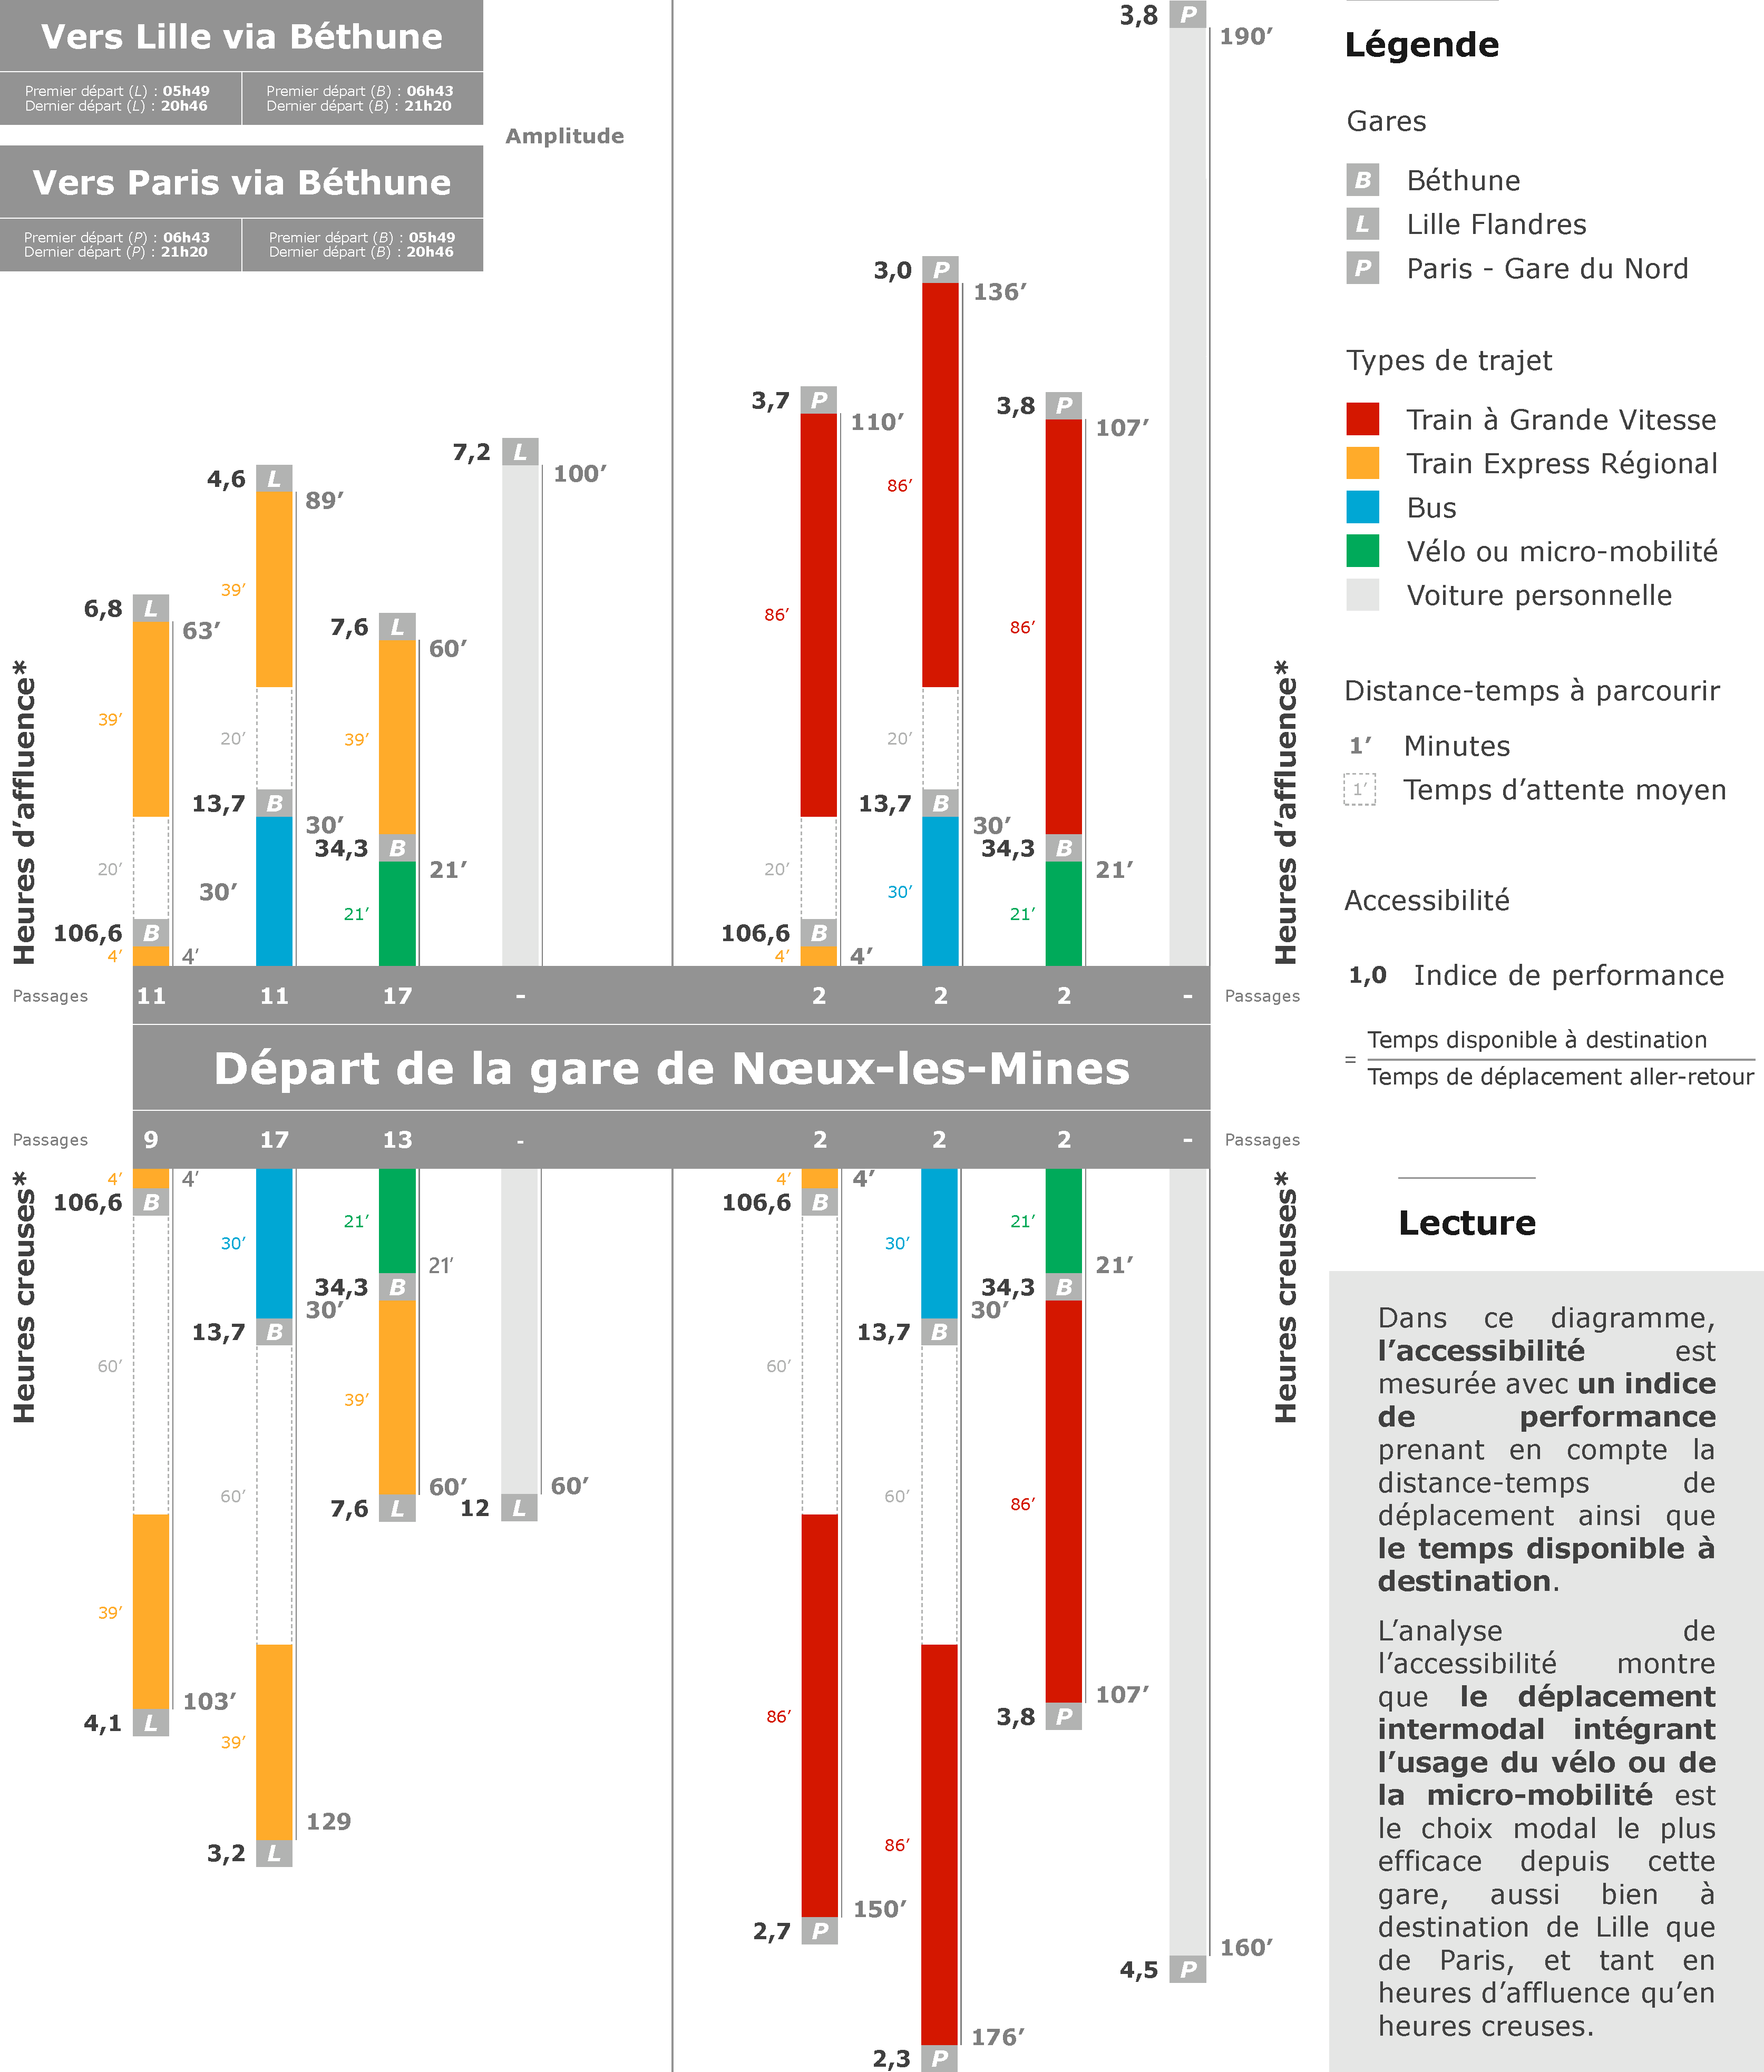
\includegraphics[width=1\columnwidth]{src/Figures/Chap-5/FR_Detours_Performance_Noeux_les_Mines.pdf}}
        \vspace{5pt}
        \begin{flushleft}\scriptsize{
        \textcolor{blue}{Note~:} les heures d'affluence correspondent à l'intervalle de temps compris entre 6h30 et 9h30 et entre 16h30 et 19h30, en semaine. Inversement, les heures creuses s'étendent de 19h30 à 6h30 et 9h30 à 16h30, en semaine.
        }\end{flushleft}
        \begin{flushright}\scriptsize{
        Jeux de données~: \acrshort{GTFS} du 27 janvier 2024 au 26 avril 2024 issues de l'\textsl{Open Data} de la \textcolor{blue}{\textcite{sncf_sncf_2022}}
        \\
        Auteur~: \textcolor{blue}{Dylan Moinse (2024)}
        }\end{flushright}
    \end{figure}

    % Littérature existante
Dans l'esprit de la géographie de l'espace-temps, se référant au courant de la \textsl{Time Geography}, cette sous-section s'attache à appliquer un indicateur fondé sur la capacité à réaliser une activité quotidienne, en tenant compte des rythmes temporels individuels. Cette perspective temporelle a été principalement adoptée par le géographe suédois \textcolor{blue}{Gunnar} \textcolor{blue}{\textcite{tornqvist_contact_1984}}\index{Törnqvist, Gunnar|pagebf}, qui a développé une méthode pour mesurer la possibilité d'établir des contacts directs, nommée \Guillemets{potentiel de contact} (\textsl{contact potential)}\footnote{Cette approche, axée sur la diffusion de l'innovation en relation avec le développement régional et la spécialisation croissante des activités, implique une augmentation du nombre de contacts entre individus.}. Comme souligné par \textcolor{blue}{\textcite[9-11]{lhostis_contribution_2018}}\index{L'Hostis, Alain|pagebf}\index{Liu, Liu|pagebf}\index{Leysens, Thomas|pagebf}, cet indicateur intégrait initialement la durée disponible à destination, la distance-temps et le coût pour un déplacement aller-retour quotidien par différents modes de déplacement. Il visait alors à illustrer les connexions existantes dans l'espace entre les lieux. Sur le plan empirique, ces \Guillemets{opportunités de contact en face-à-face} (\textsl{opportunities for face-to-face contacts}), qui se basent sur la relation entre la durée maximale de séjour et la taille de chaque population urbaine, ont été d'abord explorées dans 98 centres urbains par \textcolor{blue}{\textcite[13, 18]{tornqvist_contact_1984}}\index{Törnqvist, Gunnar|pagebf} qui a déterminé une relation linéaire entre la taille démographique de l'agglomération et le besoin de contact. \textcolor{blue}{\textcite[12]{lhostis_contribution_2018}}\index{L'Hostis, Alain|pagebf}\index{Liu, Liu|pagebf}\index{Leysens, Thomas|pagebf} notent que le traitement des correspondances et l'intermodalité sont des aspects cruciaux de la mesure de la distance-temps, qui ne sont adéquatement abordés que dans une perspective horaire. D'où l'importance d'adopter une approche basée sur les horaires pour construire des trajets monomodaux et intermodaux. Le potentiel de contact, ou la \textsl{contactabilité} \textcolor{blue}{\autocite[]{haggett_geography_2001}}\index{Haggett, Peter|pagebf}, permet alors d'analyser les relations entre villes et transport, comme l'ont étudié \textcolor{blue}{\textcite[6]{lhostis_using_2017}}\index{L'Hostis, Alain|pagebf}\index{Liu, Liu|pagebf}\index{Leysens, Thomas|pagebf} sous l'angle de l'impact de la nouvelle ligne ferroviaire à grande vitesse entre Tours et Bordeaux.%%Rédigé%%

    % Etude de cas Noeux-les-Mines : gains de temps
Dans la continuité de notre étude de cas antérieure, notre analyse se concentre sur la gare la plus proche du domicile de l'usager·ère, soit la gare de Nœux-les-Mines, en direction des pôles générateurs de flux que représentent les agglomérations de Lille et de Paris. En comparant les différents temps de déplacement ainsi que la fréquence et l'amplitude horaire de diverses combinaisons modales, nous avons cherché à évaluer les avantages comparatifs du déplacement intermodal face à un déplacement exclusivement réalisé en transport en commun ou en voiture. Comme représenté dans le \hyperref[fig-chap5:performance-detours-noeux]{graphique~\ref{fig-chap5:performance-detours-noeux}} (page~\pageref{fig-chap5:performance-detours-noeux}), la chaîne intermodale, consistant à se rendre à la gare de Béthune à l'aide d'un vélo ou d'une option de micro-mobilité avant d'emprunter le train vers Lille ou Paris, garantit un gain de distance-temps notable tant en heures de pointe qu'en heures creuses. Pour l'exemple de la gare de Nœux-les-Mines, le temps total de déplacement pour atteindre la gare Lille Flandres est réduit à 60 minutes à l'aide de cette pratique intermodale, contre 63 minutes en ayant recours au \acrshort{TER} uniquement, et à 107 minutes pour la Gare du Nord, par rapport à 110 minutes en utilisant le \acrshort{TER} et le \acrshort{TGV}. Lors des périodes de faible affluence, l'écart de temps s'accroît en faveur du déplacement intermodal impliquant un détour, avec un gain enregistré de 43 minutes pour les destinations de Lille et de Paris. Cette stratégie de détour ne se traduit pas seulement par une économie de distance-temps et une réduction des efforts liés à la rupture de charge, mais aussi par un accès à un meilleur niveau de service en matière de fréquence. Effectivement, l'usager·ère combinant la mobilité individuelle légère et le train minimise son exposition aux aléas ferroviaires et évite ainsi les désagréments liés aux correspondances, tout en accédant directement à la ligne Béthune - Lille plus régulière. Toutefois, cette observation n'est pas aussi évidente pour le scénario de déplacement intermodal en direction de la Gare du Nord, étant donné que seulement trois à quatre \acrshort{TGV} desservent quotidiennement la gare de Béthune en semaine. Malgré cela, et hormis l'économie de temps, le choix de se rendre directement à la gare de Béthune pour Paris permet à l'individu d'éviter certaines correspondances mal synchronisées entre le \acrshort{TER} et le \acrshort{TGV}, avec des temps de correspondance inférieurs à cinq minutes.%%Rédigé%%

    % Etude de cas Noeux-les-Mines : indice de performance
L'étude de cas sur l'accessibilité autour de la gare de Nœux-les-Mines nous amène à évaluer l'efficacité de la synergie entre la mobilité individuelle légère et le réseau ferroviaire, sous l'angle de la temporalité. Notre démarche, qui s'appuie sur un scénario dans lequel l'individu souhaite se rendre à Lille ou à Paris en partant de ce nœud de transport en commun, révèle que le choix d'un voyage intermodal marqué par la réalisation d'un détour permet également de profiter de meilleures opportunités temporelles à destination. En nous inspirant de \Guillemets{l'indice de performance globale}\footnote{
L'indice de performance consiste à mettre en rapport le temps maximal de séjour et le temps de voyage aller-retour \textcolor{blue}{\autocite[]{cauvin_accessibilite_1989}}\index{Cauvin-Reymond, Colette|pagebf}\index{Reymond, Henri|pagebf}\index{Schaub, Gérard|pagebf}, afin de considérer la pénibilité d'obtention de la minute disponible à destination et dès lors de mesurer l'efficacité de l'offre ferroviaire dans un contexte donné \textcolor{blue}{\autocite[130]{chapelon_transports_2016}}\index{Chapelon, Laurent|pagebf}. À travers notre étude de cas, l'indice de performance développé depuis la gare de Nœux-les-Mines se base sur la base d'un jour de semaine, en dehors des périodes de pause pédagogique, le lundi 29 janvier 2024.
} mesuré par \textcolor{blue}{Laurent} \textcolor{blue}{\textcite[130]{chapelon_transports_2016}}\index{Chapelon, Laurent|pagebf} dans son étude sur le temps disponible à Paris autour du réseau \acrshort{TGV}, l'analyse que nous avons conduite met en évidence l'efficacité temporelle offerte par le déplacement intermodal. En couplant l'usage du vélo ou de la micro-mobilité avec le \acrshort{TER} à destination de Lille, l'indice de performance atteint 7,6, en comparaison de 6,8 en période de pointe et de 4,1 en heures creuses pour le déplacement monomodal en train. Similairement, le ratio pour Paris est de 3,8, contre 3,7 en heures d'affluence et 2,7 en heures creuses. Cette lecture fondée sur les opportunités temporelles à destination démontre comment l'intégration de la mobilité individuelle légère avec le transport ferroviaire peut améliorer l'accessibilité d'un lieu (voir le \hyperref[fig-chap5:performance-detours-noeux]{diagramme~\ref{fig-chap5:performance-detours-noeux}}, page~\pageref{fig-chap5:performance-detours-noeux}). Inversement, un déplacement monomodal à vélo ou en micro-mobilité jusqu'à la gare de Béthune est peu compétitif face à l'utilisation exclusive du \acrshort{TER}, aussi bien concernant la distance-temps requise que le ratio de temps disponible sur place. Notons qu'avec le projet de \acrfull{SERM} qui desserviront les gares de Béthune et Lille Flandres, l'efficacité de la combinaison modale impliquant l'usage de la mobilité individuelle légère depuis la gare de Nœux-les-Mines sera bien plus significative et pourrait, à l'aide d'une fréquence et d'une amplitude horaire nettement améliorées, rendre ce type d'itinéraire plus compétitif que l'automobile. Toutefois, cette étude de cas dévoile certains dysfonctionnements du système de transport en commun qui tendent à réduire son attractivité~: bien que l'efficacité du voyage intermodal soit supérieure durant les heures de pointe, l'automobile s'avère plus performante durant les périodes de faible affluence en raison d'une plus amplitude horaire réduite.%%Rédigé%%

    % 5.3.4.3.
    \needspace{1\baselineskip} % Réserve de l'espace
\subsubsection*{Influence des caractéristiques socio-démographiques sur les stratégies d'optimisation
    \label{chap5:sociodemographie}
    }

    % Rôle démographie
En considérant les caractéristiques socio-démographiques du sous-échantillon obtenu se rapportant aux cyclo-voyageur·se·s ayant adopté des stratégies de détour et de pause, il est crucial de noter que ces voyageur·se·s intermodaux·les ont une répartition par \gls{genre} et par âge similaire à celle des usager·ère·s de train en France~: 39~\% de ces voyageur·se·s sont des femmes, tandis que 60~\% d'entre elleux ont entre 25 ans 45 ans, avec seulement 12~\% d'entre elleux de moins de 25 ans. Cependant, ces utilisateur·rice·s ayant recours à des trajets \acrshort{E-TVS} ont tendance à être plus souvent des professionnel·le·s employé·e·s à temps plein ou des étudiant·e·s (85~\%).%%Rédigé%%

    % Combinaison modale
Concernant leur combinaison modale, 69~\% des navetteur·se·s ayant intégré des détours ou des pauses dans leurs déplacements privilégie principalement l'utilisation du \acrshort{TER}, et jusqu'à 91~\% en faisant appel à l'ensemble des systèmes de transport en commun interurbains. Du côté de la mobilité individuelle légère, 47~\% des trajets comportant des détours ou des pauses ont été effectués à vélo personnel, 19~\% en \acrshort{TEP}, 12~\% en vélo pliant et 9~\% en \acrshort{VLS}. Cette répartition au sein du sous-échantillon étudié ne reflète pas exactement la distribution modale des modes de rabattement telle qu'observée par le cabinet d'études \textcolor{blue}{\textcite{enov_enquete_2021}}\index{Enov@\textsl{Enov}|pagebf} et par \textcolor{blue}{\textcite[180]{moinse_intermodal_2022}}\index{Moinse, Dylan|pagebf}\index{Goudeau, Matthieu|pagebf}\index{L'Hostis, Alain|pagebf}\index{Leysens, Thomas|pagebf}, qui ont rapporté une part modale égalitaire des modes de transfert, parmi le vélo conventionnel et la \acrshort{TEP}, vers le train en France.%%Rédigé%%

    % ___________________________________________
    % 5.*.
    \newpage
    \needspace{1\baselineskip} % Réserve de l'espace
    \addcontentsline{toc}{section}{Conclusion du chapitre~5}
    \sectionheader{Conclusion du chapitre}
\section*{Conclusion du chapitre~5
    \label{chap5:conclusion}
    }
    %\markright{Conclusion du chapitre~5}{}

    % Synthèse
Ce chapitre, axé sur les distances, les itinéraires et, de façon plus générale, sur l'accessibilité, a permis de mettre en lumière les avantages comparatifs de l'usage intermodal de la mobilité individuelle légère. D'une part, l'analyse des distances parcourues par les usager·ère·s révèle une extension des quartiers de gare à l'échelle locale, renouvelant ainsi la délimitation de zones stratégiques propres au \acrshort{TOD}. Cette mise en regard des cheminements cyclables nous a conduits à examiner comment le vélo et la micro-mobilité tirent parti de leur portée accrue afin de rendre le déplacement intermodal plus compétitif. Cela se traduit non seulement par une facilitation de l'accès aux réseaux de transport en commun, mais aussi par une optimisation des déplacements. D'autre part, en adoptant une perspective régionale, nous avons été en mesure d'évaluer les effets des gains d'accessibilité sur la couverture démographique et la desserte des destinations.%%Rédigé%%

    % 5.*.*
    \needspace{1\baselineskip} % Réserve de l'espace
\subsection*{Principaux enseignements
    \label{chap5:principaux-enseignements}
    }

    % Distances locales
Dans le cadre de notre premier objectif de recherche axé sur l'élargissement des quartiers de gare en fonction des différents types de véhicules propres à la mobilité individuelle légère et des facteurs influençant les distances parcourues, il a été établi que la distance spatiale jugée acceptable pour les flux pendulaires s'élève à 3,8 kilomètres de chaque côté du déplacement intermodal. Le rayon d'action pertinent pour ce corpus de modes de déplacement se situe entre 0,8 et 4,2 kilomètres pour l'étape de rabattement, et entre 0,5 et 3,3 kilomètres pour l'étape de diffusion. La marche se révèle plus compétitive en deçà de ces seuils, tandis que les transports en commun urbains et l'automobile le sont au-delà.%%Rédigé%%

    % Influence types de TC
Ces distances varient également en fonction du type de système de transport en commun utilisé, les combinaisons modales incluant l'usage du \acrshort{TGV} enregistrant une distance acceptable de quatre kilomètres, contre trois kilomètres pour le \acrshort{TER} et deux kilomètres pour le métro et le tramway. La qualité du niveau de service offert par les gares influe aussi sur ces distances, les gares offrant les meilleurs services ayant une distance acceptable de 4,8 kilomètres, contre 4,3 kilomètres pour celles proposant un service moyen et 3,8 kilomètres pour les moins attractives.%%Rédigé%%

    % Influence autres facteurs
D'autres facteurs exercent une influence positive sur la distance parcourue, tels que la fréquence d'utilisation et les \acrshort{PCS} en faveur des cadres supérieur·e·s, ainsi que le nombre d'individus dans un ménage et la substitution modale depuis la voiture pour le segment en pré-acheminement. Cela correspond à une durée moyenne de déplacement de douze minutes pour la mobilité individuelle légère en tant que mode de transfert. Il a également été observé que le même mode de déplacement est employé pour les premiers et les derniers kilomètres par plus de 83~\% des usager·ère·s du vélo pliant et par 79~\% des usager·ère·s de la \acrshort{TEP}, indiquant que les véhicules les mieux adaptés à l'embarquement à bord des modes collectifs répondent à un besoin spécifique lié à la phase de diffusion.%%Rédigé%%

    % Taille quartiers de gare
En conséquence, la délimitation des quartiers de gare piétons se trouve être 2,6 fois plus étendue pour la marche combinée, et 22,6 fois plus pour la mobilité individuelle légère, comparée aux aires d'influence communément admises. À l'échelle du déplacement global, la distance médiane d'un déplacement intermodal a été identifiée à 36 kilomètres, soit 53 minutes, avec une distance acceptable s'élevant à 71 kilomètres. La mobilité individuelle légère représente alors un cinquième de la distance spatiale, mais plus des deux tiers de la distance-temps consacrée.%%Rédigé%%

    % Accessibilité régionale
L'extension des quartiers de gare permet ainsi de couvrir 22~\% de la région à vol d'oiseau et 8~\% du territoire à partir du réseau viaire. En réponse à notre deuxième objectif, axé sur les gains d'accessibilité à l'échelle régionale, nous avons identifié une amélioration du taux d'accessibilité de la population, à hauteur de 56~\% des résident·e·s. Cela revient à desservir trois fois plus d'individus autour des gares par rapport aux aires d'influence accessibles à pied, et ce, dans des territoires quatre fois moins densément peuplés. L'intégration de la mobilité individuelle légère au réseau ferroviaire améliore considérablement la couverture de la population régionale et offre un potentiel accru pour une mobilité plus inclusive, atteignant des parcs locatifs comptant 2,4 fois plus de logements sociaux, ainsi que des zones résidentielles dont la valeur immobilière médiane est inférieure de 9,5~\% par rapport aux quartiers de gare piétons. Notre analyse des distributions géographiques des ménages selon les revenus disponibles a également mis l'accent sur un revenu médian supérieur de 3,6~\%, mais avec des écarts moins marqués entre les quartiles inférieurs et supérieurs.%%Rédigé%%

    % Accessibilité des emplois
Notre étude des transactions immobilières concernant les espaces dédiés aux secteurs industriels, commerciaux et de bureaux a démontré que les quartiers de gare plus éloignés demeurent attractifs, avec des valeurs médianes de transactions supérieures de 5~\%. Cette dynamique influence positivement l'accès aux emplois, facilitant l'accès à plus de 71~\% du marché de l'emploi, soit une augmentation de 1,76 fois le nombre d'emplois accessibles. De plus, l'accès aux \acrshort{POIs} est multiplié par 2,16, permettant d'avoir un accès potentiel à 66~\% des équipements disponibles dans la région. Plus spécifiquement, 79~\% des équipements de catégorie \Guillemets{supérieure} sont accessibles, contre 71~\% pour ceux de la gamme \Guillemets{intermédiaire} et 62~\% pour ceux de la catégorie de \Guillemets{proximité}.%%Rédigé%%

    % Détours et pauses 1
Abordant notre dernier objectif de recherche, l'identification des itinéraires sortant du périmètre de captation des stations de transport en commun, et des parcours ponctués d'arrêts intermédiaires, nous a conduits à réévaluer les relations entre les détours, les pauses et l'optimisation sous un angle intermodal. Nous avons pu conclure que les détours, lorsqu'ils sont intégrés dans des déplacements pendulaires, peuvent conduire à une économie de temps moyenne de 18~\% et à une réduction de 3~\% de la distance spatiale parcourue. En général, les navetteur·se·s dévient du trajet le plus direct, choisissant de suivre des itinéraires en rabattement et, ou bien, en diffusion trois fois plus longs, ce qui a pour effet de réduire de moitié le temps passé dans les transports en commun et de diminuer de 80~\% le temps d'attente. Un autre aspect qui ressort de ce chapitre est le regroupement des trajets analysés qui a permis de montrer que 95~\% des détours examinés aboutissent à des économies soit de distance-temps, soit de distance spatiale, tandis que 65~\% des stratégies d'optimisation réussissent à réaliser les deux simultanément.%%Rédigé%%

    % Détours et pauses 2 + Transition
L'examen de la distribution des distances montre une zone de captation des stations nettement plus vaste. Les trajets \acrshort{E-TVS} s'étendent typiquement de cinq à six kilomètres, ce qui équivaut à une durée de vingt minutes. Nous pouvons ainsi déduire que les voyageur·se·s sont disposé·e·s à réaliser deux kilomètres supplémentaires de détour, étendant de 2,3 fois la zone de service des gares et de 19,9 fois la taille de l'\Guillemets{aire primaire}. Il est démontré que la direction prise lors des déplacements intermodaux influence leur efficacité. Les gains de temps sont plus significatifs lorsque les détours impliquent une forme extrême de détour, telle qu'une inversion spatiale. Par ailleurs, les pauses fournissent une occasion de tirer parti des temps d'attente. Ces interruptions sont généralement consacrées à des achats quotidiens, s'inscrivant dans le cadre d'une chaîne de déplacement plus complexe. En somme, ces deux chapitres se sont attachés à mesurer et à expliquer l’extension spatiale des quartiers de gare induite par la mobilité individuelle légère, dans le but d’évaluer les gains d’accessibilité intermodale qu’elle permet. À la différence de ces chapitres fondés sur une approche par l'\Guillemets{accessibilité effective}, qui vise à diagnostiquer les conditions d’accessibilité réelles, le prochain volet de la recherche doctorale se penche sur l'\Guillemets{accessibilité normative}, cherchant à formuler des préconisations pour améliorer l’accessibilité, tout en garantissant leur faisabilité \textcolor{blue}{\autocite[19]{levine_mobility_2019}}\index{Levine, Jonathan|pagebf}\index{Grengs, Joe|pagebf}\index{Merlin, Louis~A.|pagebf}.%%Rédigé%%

% ___________________________________________
     \newpage
     
% Valorisation scientifique
    \begin{tcolorbox}[colback=white!5!white,
                      colframe=blue!75!blue,
                      title=Valorisation scientifique
                      \\
                      Chapitre~5]
\Large{\textcolor{blue}{\textbf{Publication dans des revues avec comité de lecture~:}}}
    \\\\
\small{\textcolor{blue}{\textcite{moinse_optimizing_2024}}\index{Moinse, Dylan|pagebf}\index{L'Hostis, Alain|pagebf}. Optimizing Intermodal Commuting by way of Detours and Breaks: Evidence of Micromobility Users in France. \textsl{Journal of Transport Geography}. 116(103821), (1-16~p.).
\\
\footnotesize{\url{https://doi.org/10/gtkvs9}} (\textbf{ACL})}
    \\\\
\Large{\textcolor{blue}{\textbf{Congrès internationaux~:}}}
    \\\\
\small{\textcolor{blue}{\textcite{moinse_optimizing_2023}}. Optimizing intermodal commuting by way of detours and breaks. Evidence of micromobility users in France. \textsl{World Conference on Transport Research} (WCTR), Montréal. 
\\
\footnotesize{\url{https://hal.science/hal-04166574}} (\textbf{C-ACTI})}
    \\\\
\Large{\textcolor{blue}{\textbf{Manifestations scientifiques~:}}}
    \\\\
\small{\textcolor{blue}{\textcite{moinse_eclater_2022}}. Éclater la bulle des périmètres du Transit-Oriented Development (TOD). Vers un Micromobility-based TOD à l'échelle régionale ? \textsl{Rencontres TerriTrans - MoTAU}, Aix-en-Provence. 
\\
\footnotesize{\url{https://hal.science/hal-03881592}} (\textbf{C-COM})}
    \\\\
\small{\textcolor{blue}{\textcite{moinse_analysis_2021}}. An Analysis of Intermodal Use of e-Scooters with train in the Provence-Alpes-Côte d’Azur Region, in France: Towards Extended Railway Station Areas? \textsl{Smart And Sustainable Cities Conference}, \textsl{Urban mobility, New Technologies and Urban Development}, Paris.
\\
\footnotesize{\url{https://shs.hal.science/halshs-03507433}} (\textbf{C-ACTI})}
    \\\\
\small{\textcolor{blue}{\textcite{moinse_analyse_2021}}. Une analyse de l’usage intermodal des trottinettes avec le train dans la région Provence-Alpes-Côte d’Azur. Vers une extension des quartiers de gare~? \textsl{Future Days}, Mobilité décarbonée, Paris.
\\
\footnotesize{\url{https://hal.science/hal-03473394}} (\textbf{C-COM})}
    \\\\
\Large{\textcolor{blue}{\textbf{Vulgarisation scientifique~:}}}
    \\\\
\small{\textcolor{blue}{\textcite{moinse_trottinettes_2022}}. \textsl{Des trottinettes pour « éclater la bulle » des transports en commun}, Fête de la Science : Ateliers 1 classe, 1 scientifique, 1 heure, Paris 
\\
\footnotesize{\url{https://shs.hal.science/halshs-03810191}}}
    \\\\
\small{\textcolor{blue}{\textcite{moinse_jpeux_2022}}. J’peux pas prendre le train, j’vis trop loin de la gare pour y aller à pied, \textsl{Revue d'Urbanisme et d'Expression Urbaine lÂme Urbaine}, 12, 15~p.
\\
\footnotesize{\url{https://www.asso-envar.com/la-revue}}}
    \\\\
\small{\textcolor{blue}{\textcite{moinse_temps_2020}}. Le temps dans les transports. Cadeau ou fardeau~? \textsl{Revue d'Urbanisme et d'Expression Urbaine lÂme Urbaine}, 11, 17~p.
\\
\footnotesize{\url{https://www.asso-envar.com/la-revue}}}
    \end{tcolorbox}

    % ___________________________________________
    % Sous-bibliographie
    \newpage
    \sectionheader{Sous-bibliographie du chapitre~5}
    \begingroup
    \renewcommand{\bibfont}{\scriptsize}
\printbibliography[segment=\therefsegment, heading=subbibintoc, title={Sous-bibliographie du chapitre~5}, label=chap5:bibliographie]
    \endgroup
    \end{refsegment}